%% main_paper_NN29.tex
%% Neural Networks 投稿用日本語草稿
%% AE/VAEにおける有効潜在次元の診断的解釈（版29）
%% コンパイル: platex main_paper_NN29.tex && dvipdfmx main_paper_NN29.dvi

\documentclass[11pt,a4paper]{jsarticle}

\usepackage{amsmath,amsthm,amssymb}
\usepackage{mathtools}
\usepackage[dvipdfmx]{graphicx}
\usepackage{booktabs}
\usepackage{url}
\usepackage{here}
\usepackage{array}
\usepackage{multirow}
\usepackage{enumerate}
\usepackage[margin=25mm]{geometry}
\usepackage[dvipdfmx,hidelinks]{hyperref}
\usepackage{caption}

%% 定理環境
\newtheorem{theorem}{定理}
\newtheorem{proposition}{命題}
\newtheorem{definition}{定義}
\newtheorem{remark}{注意}
\newtheorem{corollary}{系}

%% 記号略記
\newcommand{\dID}{d_{\mathrm{ID}}}
\newcommand{\dz}{m}
\newcommand{\dzopt}{m^{\mathrm{cand}}}
\newcommand{\dtrue}{d_{\mathrm{true}}}
\newcommand{\Jg}{J_g}
\newcommand{\R}{\mathbb{R}}
\newcommand{\kap}{\kappa}
\newcommand{\AUsat}{\mathrm{AU}_{\mathrm{sat}}}
\newcommand{\dzsat}{m^{\mathrm{sat}}}
\newcommand{\mknee}{m^{\mathrm{knee}}}
\newcommand{\demb}{d_{\mathrm{emb}}}

%% ===================================================================
\title{AE/VAE における有効潜在次元の診断的解釈}
%% 英語タイトル候補：
%%   Diagnostic Interpretation of Effective Latent Dimensionality in
%%   Autoencoders and Variational Autoencoders
%%   （または）
%%   Interpreting Effective Latent Dimensionality in AE/VAE Models via
%%   Active-Unit Dynamics and Intrinsic Dimension Estimation
\author{（著者名）\\
{\small （所属機関）}\\
{\small \texttt{（メールアドレス）}}}
\date{}

\begin{document}
\maketitle

%% ===================================================================
\begin{abstract}
本論文は，AE/VAE が学習した潜在表現において実際に利用される有効潜在次元を診断するため，
Active Unit（AU）Dynamics，内在次元（ID）推定（TwoNN/MLE），MSE エルボー，PCA を組み合わせた
\textbf{多指標診断フレームワーク}を提案する．
本フレームワークは，有効潜在次元を単一の数値として一意に決定することを目的とせず，
AU 値を頑健な直接観測指標，TwoNN ID を数値的に安定な補助的参照推定量，
AU 鈍化点$\mknee$をグリッド・シード依存性をもつ探索的指標として明確に区別する．

理論面では，線形ガウス $\beta$-VAE の rate-distortion 近似のもとで，
データ共分散の第$j$固有値$\lambda_j$，デコーダノイズ分散$\tau^2$，正則化係数$\beta$に対する
AU 活性化条件$\lambda_j > \beta\tau^2$を導出し，AU 飽和と$\mknee$のグリッド感度を
説明する理論的基盤を与える．

実験面では，MNIST の全結合 VAE において AU 値と TwoNN ID が複数シードにわたり
高い再現性を示すことを確認した（例：TwoNN ID $= 10.03 \pm 0.12$）．
一方，$\mknee$は疎グリッドでは大きく変動したが，
推定 ID 近傍を密に探索し複数シードで評価することで
$\mknee = 10.3 \pm 0.9$ と TwoNN ID 近傍に安定化することを示した．
さらに Fashion-MNIST，Conv-VAE，CIFAR-10/SVHN 実験により，
本診断フレームワークが有効に機能する条件と，
AU/$\mknee$ 診断が困難となる境界条件を定量化した．
\end{abstract}

%% ===================================================================
\section{まえがき}\label{sec:intro}

\subsection{研究背景：有効潜在次元の解釈という問題}\label{sec:intro_bg}

表現学習において，オートエンコーダ（Autoencoder; AE）および
変分オートエンコーダ（Variational Autoencoder; VAE）\cite{kingma2014vae}は，
高次元データから低次元の潜在表現（latent representation）を学習する
中核的な非教師あり学習モデルである\cite{bengio2013representation}．
この潜在表現の「質」を規定する最も基本的な設計パラメータが
ボトルネック次元（bottleneck dimension）$m$である：
$m$が小さすぎると情報が欠落し，大きすぎると
冗長な次元が生じる（VAE では posterior collapse\cite{lucas2019elbo}が悪化する）．

しかし，学習された潜在表現が「実際に何次元を有効に使っているか」——
すなわち\textbf{有効潜在次元（effective latent dimensionality）}——を
定量的に読む方法論は，深層表現学習の研究において十分に確立されていない．
既存研究\cite{ansuini2019intrinsic,valeriani2023geometry}は
深層ネットワークの各層の内在次元を測定してきたが，
AE/VAE のボトルネックにおける有効次元を，その学習ダイナミクスとともに
系統的に分析した研究は限られている．

本論文が取り組む中核的な問いは：
\begin{quote}
\textit{AE/VAE は，入力データの内在次元（local intrinsic dimensionality）や
位相的埋め込み次元（topological embedding dimensionality）をどのように
潜在空間の有効次元として「学習」するか？
そして，その有効次元を外から定量的に読む方法はあるか？}
\end{quote}

\subsection{本研究の位置づけと貢献}\label{sec:intro_aim}

本論文では，この問いに対し，
\textbf{内在次元（ID）推定}と\textbf{Active-Unit（AU）Dynamics}を柱とした
\textbf{多指標診断フレームワーク}を提案する．
本フレームワークの核心は，有効次元を単一指標で「一意に決定」するのではなく，
各指標の頑健性と探索的性格を明示した上で組み合わせ，\textbf{診断的に解釈する}点に新規性がある．
「$\mknee$ により適切なボトルネック次元を一意に同定できる」という主張は行わない——
$\mknee$ は設計の粗い探索的目安であり，主要な有効次元の読み取りは
頑健指標（AU 値）と数値安定な補助的参照推定量（TwoNN ID）が担う．

\textbf{各指標の役割と頑健性}：
\begin{itemize}
  \item \textbf{TwoNN/MLE ID}：局所距離から有効自由度を推定する数値的に安定な補助的参照推定量
        （シード間$\sigma \leq 0.12$；等長性バイアスあり；§\ref{sec:exp_multiseed2}）．
  \item \textbf{AU 値}：KL 正則化された VAE が各次元を実際に使用しているかを直接観測する頑健な指標
        （シード間$\sigma \leq 0.5$；参照 AE の距離保存性には非依存；$\beta$・$\delta$・モデル容量に依存）．
  \item \textbf{MSE エルボー・PCA}：再構成誤差側からの補助的な有効次元の読み取り．
  \item \textbf{AU 鈍化点$\mknee$}：上記の AU 曲線形状から導かれる探索的指標——
        KL 正則化が次元圧縮を開始する転換点を粗く捉えるが，
        数値は$m$グリッド・乱数シードに依存する（§\ref{sec:exp_multiseed2}）．
\end{itemize}

本論文の\textbf{貢献は以下の3点}である：
\begin{enumerate}
  \item \textbf{多指標診断フレームワークの提案}：
        AE/VAE の有効潜在次元を，AU 値，TwoNN/MLE ID，MSE エルボー，PCA から診断的に読み取る
        フレームワークを提案する．
        AU 値を潜在次元の利用状況を直接観測する頑健指標，
        TwoNN ID を数値的に安定な補助的参照推定量，
        $\mknee$を AU 曲線形状から得られる探索的変化点として明確に区別する
        （§\ref{sec:framework}，§\ref{sec:discussion}）．
        MNIST での3シード検証により AU 値（$\sigma \leq 0.5$）と TwoNN ID（$10.03 \pm 0.12$）の
        高い再現性を確認し，密グリッド・独立初期化・複数シード条件での
        $\mknee = 10.3 \pm 0.9$（Exp-Mnist-Dense-300）を主要な安定化結果とする（§\ref{sec:exp_el}）．
  \item \textbf{線形ガウス rate-distortion 近似に基づく AU 活性化条件の導出}：
        線形ガウス $\beta$-VAE の rate-distortion 近似のもとで，
        第$j$潜在次元が活性となる条件$\lambda_j > \beta\tau^2$を
        水充填定理と KKT 条件から導出し（定理\ref{thm:linear_vae}，§\ref{sec:theory}），
        KL 正則化が有効次元を抑制する機構を水充填原理の観点から説明する．
        本結果は実際の非線形 VAE の厳密定理ではなく，線形ガウス rate-distortion 近似に基づく
        解析結果として，非線形実験との定性的対応を与えるものである．
  \item \textbf{適用可能範囲と限界条件の定量化}：
        MNIST/Fashion-MNIST（FC-VAE），Conv-VAE，CIFAR-10/SVHN を対象に，
        AU 値・TwoNN ID の再現性，$\mknee$のグリッド・シード依存性，
        および「等長性改善より$m \gg \hat{d}_\mathrm{ID}$が TwoNN 安定性の支配的条件」
        （Exp-Real-Geom，命題\ref{thm:twonn_stability}）を実証する．
        さらに Conv-VAE・自然画像では，AU/$\mknee$ 診断が困難となる境界条件を
        stable identification の5条件（operational criteria）として定量化する
        （§\ref{sec:disc_convvae}，§\ref{sec:disc_limitation}）．
\end{enumerate}

\subsection{「次元」の2種類：局所的固有次元と位相的埋め込み次元}\label{sec:intro_dim}

本論文では多様体の「次元」として$\dID$（局所的固有次元：TwoNN/MLE の推定対象）と
$\demb$（位相的最小埋め込み次元：自己交差なく埋め込むための最小次元）を区別する
（Swiss Roll では$\demb = \dID = 2$，Torus では$\demb = 3 > \dID = 2$）．

ただし，\textbf{本論文の主貢献は$\dID$や$\demb$との対応を証明することではなく，
AU 値・TwoNN ID・$\mknee$という診断指標の頑健性・限界・適用条件の整理にある}．
$\demb$と$\AUsat$との条件付き対応（Torus・Möbius 等）は付随的観察として補助に位置づける
（§\ref{sec:disc_incidental}）．

\subsection{リサーチクエスチョン}\label{sec:intro_rq}

\begin{description}
  \item[RQ1] VAE の AU Dynamics から得られる変化点$\mknee$は，どのようなグリッド密度・シード数・
             アーキテクチャ条件のもとで，TwoNN/MLE による ID 推定値と整合する診断補助量として
             利用可能か．
  \item[RQ2] AE/VAE の有効潜在次元を多指標（AU 値，TwoNN/MLE，MSE エルボー，PCA）で
             解釈するフレームワークは，単一指標に対して相補的な情報を提供するか．
  \item[RQ3] ボトルネック余裕（$m / \hat{d}_\mathrm{ID}$ の大小）および幾何的正則化（IsometricAE）は，
             TwoNN ID 推定の安定性にどのような影響を与えるか．
\end{description}

\subsection{本論文の構成}\label{sec:intro_structure}

\textbf{検証範囲の明示}：
本論文の検証は合成多様体（$d_{\mathrm{true}} \leq 3$）・MNIST・Fashion-MNIST（全結合型 AE/VAE），
Conv-AE/VAE（実験 Exp-Conv-AE・Exp-Conv-Fix），KL アニーリング（実験 Exp-Conv-Ann），
および自然画像（CIFAR-10・SVHN；実験 Exp-Nat-Cifar・Exp-Nat-SVHN）を対象とする．
自然画像実験（Exp-Nat-Cifar・Exp-Nat-SVHN）では，TwoNN 補助推定が Pope ら\cite{pope2021intrinsic}の
報告値と整合する推定値を与えることを確認し，
さらに Conv-VAE における AU/$\mknee$ 診断の適用可能範囲（validity range）と限界条件を定量化する
（フレームワーク全体の自然画像への「汎化」を主張するものではない）．

§\ref{sec:related}（関連研究），§\ref{sec:framework}（フレームワーク），
§\ref{sec:theory}（理論的背景；定理\ref{thm:linear_vae}含む），
§\ref{sec:exp}（実験），§\ref{sec:discussion}（考察），§\ref{sec:conclusion}（むすび）の順で構成する．
詳細な証明と感度分析は付録にまとめる．

%% ===================================================================
\section{関連研究}\label{sec:related}

\subsection{表現学習とオートエンコーダ}\label{sec:related_ae}

Bengio ら\cite{bengio2013representation}は表現学習の理論的枠組みを整理し，
AE が多様体仮説\cite{fefferman2016manifold}に基づいて
高次元データの低次元構造を学習する機構を論じた．
$\beta$-VAE\cite{higgins2017betavae}は KL 正則化の重み$\beta$を大きくすることで
Disentangled 表現を促進し，AU に直接影響する．
Lucas ら\cite{lucas2019elbo}は，VAE の ELBO 最小化において
posterior collapse（AU の大幅な減少）が生じる条件を線形 VAE の枠組みで分析し，
AU が$d_{\mathrm{ID}}$近傍で飽和することを理論的に示した．
DAE\cite{alain2014dae}はスコアマッチングの観点から，
Denoising Autoencoder の再構成方向が多様体の法線方向を選択的に抑制することを示した．
CAE\cite{rifai2011cae}はエンコーダ側ヤコビアンの正則化により収縮的表現を学習する．

\subsection{深層表現の内在次元解析}\label{sec:related_id}

Pope ら\cite{pope2021intrinsic}は自然画像の内在次元が
TwoNN 推定で画素次元よりはるかに低いことを示した
（CIFAR-10: $d_\mathrm{ID} \approx 26$ at $32 \times 32$）．
Ansuini ら\cite{ansuini2019intrinsic}は深層ネットワークの各層を通じて
ID が変化するパターンを定量化し，表現の収縮・拡張現象を記録した．
Valeriani ら\cite{valeriani2023geometry}は大規模変換器モデルの隠れ表現の
幾何構造を系統的に解析した．
Birdal ら\cite{birdal2021intrinsic}は持続的ホモロジーと ID の統合による
汎化誤差との関係を分析した．
本研究はこれらの「既存のネットワークの ID を測る」研究と相補的であり，
AE/VAE の\textbf{設計段階}および\textbf{学習ダイナミクス}における有効次元の形成を追跡する点で異なる．

内在次元推定手法としては，TwoNN\cite{facco2017twonn}（2近傍距離比）と
MLE\cite{levina2005mle}（最尤推定）を採用する．
DANCo\cite{ceruti2014danco}はより精密だが計算コストが高い．
なお，非線形次元削減の可視化手法として UMAP\cite{mcinnes2018umap}が広く用いられるが，
本研究は可視化ではなくボトルネック次元の\textbf{定量的な解釈}に焦点を当てる．

\subsection{Active Units と Posterior Collapse}\label{sec:related_au}

Active Unit（AU）\cite{lucas2019elbo,higgins2017betavae}は，
VAE の事後平均の分散が閾値$\delta$を超える潜在次元の数であり，
KL 正則化が有効に機能している次元数を定量化する指標である．
Lucas ら\cite{lucas2019elbo}は，ELBO の最小化が posterior collapse を引き起こし，
AU が$d_{\mathrm{ID}}$付近で飽和することを線形 VAE の枠組みで示した．
一方，本研究の定理\ref{thm:linear_vae}は Lucas らの定性的議論を，
データ固有値$\lambda_j$・ノイズ$\tau^2$・正則化$\beta$による
\textbf{閉形式しきい値$\lambda_j > \beta\tau^2$として定量化}し，
さらに Shannon の水充填定理との明示的な結びつきと KKT 条件を用いて，
線形ガウス rate-distortion 近似のもとで定量的導出を行う点が新規性である
（Tipping \& Bishop~\cite{tippingbishop1999ppca}の PPCA における$\beta=1$の特殊ケースも統合する）．
また，実データにおける AU 増加ダイナミクスの系統的な分析，特に$\mknee$という概念とその
有効表現次元との対応・限界条件・安定化戦略については，本研究が体系的に検証する
（定理\ref{thm:linear_vae}，命題\ref{thm:mknee_instab}，§\ref{sec:disc_mknee_improve}）．

\subsection{幾何的オートエンコーダ}\label{sec:related_geo}

Nazari ら\cite{nazari2023geometric}は幾何的オートエンコーダを提案し，
エンコーダが多様体の幾何構造を保存するための正則化を導入した．
Kato ら\cite{kato2020rdae}はデコーダのヤコビ行列に対するプルバック計量の
単位行列への近似化により等長埋め込みを実現する IsometricAE を提案した．
本研究では IsometricAE を「有効次元の読み取り精度の前提条件（等長性）を
改善する補助ツール」として位置づける（RQ3，実験 Exp-Syn-Iso）．

%% ===================================================================
\section{フレームワーク：有効潜在次元の読み取り}\label{sec:framework}

\subsection{問題設定と主要記号}\label{sec:framework_setup}

AE/VAE を入力次元$N$，ボトルネック次元$m$で定義する：
エンコーダ$f: \R^N \to \R^m$，デコーダ$g: \R^m \to \R^N$．
VAE ではエンコーダが事後分布$q_\phi(z|x) = \mathcal{N}(\mu(x), \sigma^2(x))$を出力し，
KL 正則化（強度$\beta$）が情報ボトルネックとして作用する．

\textbf{Active Unit（AU）}の定義：
\begin{equation}
  \mathrm{AU}(m) = \sum_{k=1}^{m} \mathbf{1}\bigl[\mathrm{Var}_x[\mu_k(x)] > \delta\bigr],
  \quad \delta = 10^{-2}
  \label{eq:au_def}
\end{equation}
ただし$\mu_k(x)$は事後平均の第$k$成分，$\delta$は閾値（Lucas ら\cite{lucas2019elbo}に準拠）．
この閾値選択に対して AU は極めて頑健であり，$\delta \in [10^{-3}, 10^{-1}]$の範囲で AU 値はほぼ変化しないことを感度分析で確認している（\ref{app:delta}参照）．

\textbf{AU 正規化増加率}$r(m)$：
\begin{equation}
  r(m) = \frac{\mathrm{AU}(m) - \mathrm{AU}(m_{\mathrm{prev}})}{m - m_{\mathrm{prev}}} \cdot \frac{1}{r_{\max}}
  \label{eq:au_rate}
\end{equation}
ただし$m_{\mathrm{prev}}$はグリッド上の直前の$m$値，$r_{\max} = \max_{m'} r(m')$．

\textbf{主要記号一覧}を表\ref{tab:notation}に示す．

\begin{table}[H]
\centering
\caption{Notation used throughout this paper}
\label{tab:notation}
\small
\begin{tabular}{lll}
\toprule
Symbol & Meaning & Section \\
\midrule
$m$ & Bottleneck dimension (design parameter) & §\ref{sec:framework} \\
$\dzopt$（$= m^{\mathrm{cand}}$） & Diagnostic candidate dimension (not a unique optimum) & §\ref{sec:framework} \\
$\dzsat$（$= m^{\mathrm{sat}}$） & AU sharp saturation point (diagnostic candidate for synthetic manifolds) & §\ref{sec:framework} \\
$\mknee$（$= m^{\mathrm{knee}}$） & AU slowdown point (rough heuristic for real data) & 式\eqref{eq:mknee} \\
$\AUsat$ & Maximum AU value over the grid & 式\eqref{eq:au_def} \\
$\hat{\dID}$ & ID estimate via TwoNN/MLE & §\ref{sec:framework} \\
$\dtrue$ & True intrinsic dimension of synthetic manifold (known) & §\ref{sec:exp_synthetic} \\
$\demb$ & Topological minimum embedding dimension ($\demb \geq \dID$) & §\ref{sec:intro_dim} \\
$\kap$ & Decoder Jacobian condition number (isometry indicator) & §\ref{sec:related_geo} \\
$r(m)$ & Normalized AU increase rate & 式\eqref{eq:au_rate} \\
$\tau_{\mathrm{knee}}$ & Slowdown detection threshold (default: 0.25) & 式\eqref{eq:mknee} \\
\bottomrule
\end{tabular}
\end{table}

本フレームワークの核心は，各指標を\textbf{頑健指標}と\textbf{探索的指標}に明示的に分類した上で
相補的に活用する点にある（表\ref{tab:indicator_class}）．
この分類は，後述の実験的知見（§\ref{sec:exp_multiseed2}）に基づく実証的分類であり，
単一指標への過信が招く誤診断を体系的に回避する設計思想の中核をなす．

\begin{table}[H]
\centering
\caption{Classification and empirical reliability of diagnostic indicators}
\label{tab:indicator_class}
\small
\begin{tabular}{p{3.5cm}p{3.2cm}p{4.0cm}p{4.0cm}}
\toprule
Indicator & Category & Empirical reliability (inter-seed $\sigma$) & Primary use \\
\midrule
AU values ($\mathrm{AU}(m)$) & \textbf{Robust indicator} & $\sigma \leq 0.5$ (MNIST 300ep) & Direct observation of effective dimensionality; independent of reference AE geometry (depends on $\beta$, $\delta$, model capacity) \\
TwoNN ID ($\hat{d}_\mathrm{ID}$) & \textbf{Numerically stable auxiliary reference}$^\dagger$ & $\sigma \leq 0.12$ ($m=64$) & Reference estimate of intrinsic dimension \\
MSE elbow & Auxiliary indicator & Qualitative only & Reconstruction-side verification \\
PCA cumulative variance & Auxiliary indicator & Linear assumption only & Linear baseline \\
$\mknee$ (AU slowdown point) & \textbf{Exploratory indicator} & $\sigma=15$ (sparse grid); $\sigma=0.9$ (dense grid) & Rough heuristic of effective dimensionality \\
\bottomrule
\end{tabular}
\medskip
\footnotesize
$^\dagger$ TwoNN ID is a \textbf{supplementary reference estimator} subject to isometry bias ($\kap \approx 10^9$); see §\ref{sec:framework_pipeline} for details.
$\sigma$ of $\mknee$ is for sparse grid; improved to $\sigma=0.9$ with dense grid (Exp-Mnist-Dense), where grid design is a major factor (§\ref{sec:exp_el}).
\normalsize
\end{table}

\begin{remark}[用語の整理]
本稿では以下の用語を使い分ける：
\textbf{有効潜在次元}（effective latent dimensionality）は，AE/VAE が実際に活用している
ボトルネック次元数の総称であり，設計者が知りたい量である．
\textbf{$\hat{d}_\mathrm{ID}$}（推定内在次元）は TwoNN/MLE による点推定値（参照 AE 経由，等長性バイアスあり）を指す．
\textbf{$\mknee$}は VAE の AU Dynamics から読み取る有効次元の観測的指標を指す．
\textbf{$\AUsat$}はグリッド上の最大 AU 値（合成多様体では飽和値，実データでは参考値）を指す．
これらはいずれも「有効潜在次元」の異なる近似・観測手法による推定値であり，
原理的には一致を期待できる（本研究条件下での経験的確認；§\ref{sec:exp}）．
\end{remark}

\subsection{有効潜在次元の読み取りパイプライン}\label{sec:framework_pipeline}

本研究が提案するフレームワークは，
「AE/VAE が学習する有効潜在次元を2段階で読み取る」解釈パイプラインである（図\ref{fig:framework}）．

\textbf{Stage 1：内在次元の近似推定（補助的役割）}

本論文では，内在次元$\hat{d}_\mathrm{ID}$の推定を2通りの方法で行う：
（a）\textbf{合成多様体}では入力空間に直接 TwoNN/MLE を適用（$\dtrue$との対比が可能）；
（b）\textbf{実データ（MNIST 等）}では，高次元の呪いを回避するため，
大きめの参照 AE（$m_{\mathrm{ref}} = 256$）の潜在表現を経由して推定する．

\textbf{限界の明示}：方法（b）の参照 AE（$m = 256 \gg \hat{d}_\mathrm{ID}$）の潜在空間は
等長性を保証しておらず（補助測定：$\kap \approx 10^9$；§\ref{sec:disc_limitation}），
得られた$\hat{d}_\mathrm{ID}$は等長性バイアスを含む近似値である．
本論文では，$\hat{d}_\mathrm{ID}$を$\mknee$の候補範囲を示す\textbf{補助的な事前情報}として扱い，
主要な有効次元の読み取りは Stage 2 の AU Dynamics に委ねる設計とする．
これにより，参照 AE の非等長性に由来する循環的な議論を避ける．
複数の$m$値（例：$\{64, 128, 256\}$）での推定値が収束していることを確認することで，
実用上の安定性を担保する．

\textbf{Stage 2：AU Dynamics による有効次元の読み取り}

ボトルネック次元$m$を離散グリッド
$\mathcal{M} = \{1, 2, 4, 8, 12, 16, 20, 32, 64, 128, 256\}$上でスイープし，
各$m$で VAE（$\beta = 4$）を学習して AU$(m)$を計算する．
AU パターンに応じて診断候補次元$\dzopt$（$= m^{\mathrm{cand}}$）の読み取り方を使い分ける
（\textbf{$\dzopt$はボトルネック次元の唯一の「最適値」ではなく，多指標による診断上の候補次元である}）：

\begin{description}
  \item[飽和型（合成多様体などシンプルなデータ）]
        AU が特定の$m$で急激に飽和する場合，その飽和点$\dzsat$を
        診断候補次元$\dzopt = \dzsat$として用いる
        （AU 値が頑健なため，この条件ではかなり信頼性が高い）．
  \item[漸増型（実データ，MNIST 等）]
        AU が$m$とともに緩やかに増加する場合，鈍化点$\mknee$を
        粗い設計目安として参照する（探索的指標）：
        \begin{equation}
          \mknee = \min\{m \in \mathcal{M} : r(m) < \tau_{\mathrm{knee}} \cdot r_{\max}\}
          \label{eq:mknee}
        \end{equation}
        ただし$\tau_{\mathrm{knee}} = 0.25$（デフォルト；\ref{app:tau_knee}参照）．
        $\mknee$は「VAE が最初に有意な次元圧縮を行う点」を粗く捉えるが，
        数値は$m$グリッドや乱数シードに依存するため，
        AU 値・TwoNN ID と照合して最終的に判断する（§\ref{sec:disc_mknee}）．
        $\mknee$と$\hat{d}_\mathrm{ID}$が整合しなくてもフレームワーク全体が無効になるわけではない．
\end{description}

CKA\cite{kornblith2019cka}および MSE エルボーを補助基準として多指標で総合的に判断する．

\begin{figure}[H]
\centering
\renewcommand{\arraystretch}{1.4}
\begin{tabular}{c}
  \fbox{\textbf{入力データ} $\boldsymbol{X} \in \R^N$（多様体仮説のもと）} \\[3pt]
  $\Big\downarrow$ \\[1pt]
  \fbox{\parbox{0.70\linewidth}{\centering
    \textbf{Stage 1：有効内在次元の近似推定}\\[1pt]
    合成多様体（$\dtrue$既知）でベンチマーク → TwoNN/MLE を選択\\
    実データ：参照 AE（$m_{\mathrm{ref}} = 256$）の潜在表現で TwoNN/MLE を適用\\
    $\Rightarrow$ 推定値 $\hat{\dID}$（候補範囲の目安，近似値）
  }} \\[3pt]
  $\Big\downarrow$ \\[1pt]
  \fbox{\parbox{0.70\linewidth}{\centering
    \textbf{Stage 2：AU Dynamics による有効次元の診断}\\[1pt]
    グリッド$\mathcal{M}$上で VAE をスイープ → AU$(m)$ を追跡\\
    飽和型：診断候補 $\dzopt = \dzsat$（信頼性高），漸増型：粗い目安 $\dzopt = \mknee$（探索的）\\
    \textbf{主要指標}：AU 値（頑健指標）・TwoNN ID（数値安定な補助的参照）\\
    \textbf{$\mknee$は探索的目安であり，一意な最適値ではない}
  }} \\[3pt]
  $\Big\downarrow$ \\[1pt]
  \fbox{\parbox{0.70\linewidth}{\centering
    \textbf{補助（RQ3）：幾何的正則化・ボトルネック余裕と TwoNN 安定性の確認}\\[1pt]
    $m \gg \hat{d}_\mathrm{ID}$の条件確認 → TwoNN 補助推定の適用条件（validity range）を評価
  }}
\end{tabular}
\caption{Diagnostic pipeline for effective latent dimensionality. The diagnostic candidate dimension $\dzopt$ is not a unique optimal solution but a candidate based on multiple indicators (AU values, TwoNN ID, $\mknee$).}
\label{fig:framework}
\end{figure}

\subsection{$\mknee$ の解釈的意義}\label{sec:framework_mknee_interp}

$\mknee$が有効表現次元の指標として機能するメカニズムを以下に述べる．

VAE の ELBO を最小化する過程で，KL 正則化（情報ボトルネック項）は
再構成に必要でない余剰潜在次元を非活性化する（posterior collapse を誘導する）
\cite{lucas2019elbo,higgins2017betavae}．
$m < \hat{d}_\mathrm{ID}$の段階では，ボトルネックが再構成の妨げとなるため，
VAE は利用可能な全ての次元を AU として活性化させる（$\mathrm{AU}(m) \approx m$）．
$m \approx \hat{d}_\mathrm{ID}$を超えると，余剰次元が生じ始め，
KL 正則化がそれらを非活性化する圧力を加えるため，AU の増加率が鈍化する．
この鈍化点$\mknee$は，特定の条件下（Fashion-MNIST 等）でデータの有効内在次元$\hat{d}_\mathrm{ID}$と
整合する傾向が観測されるが，数値的な再現性は$m$グリッドや乱数シードに依存し保証されない
（§\ref{sec:exp_multiseed2}，§\ref{sec:disc_mknee}）．
フレームワークとしては，$\mknee$の整合有無にかかわらず，
AU 値（頑健な直接観測量）と TwoNN ID（数値安定な補助的参照推定量）の組み合わせによる
有効次元の読み取りが，本フレームワークの中心的な知見である．

%% ===================================================================
\section{理論的背景}\label{sec:theory}

本章では，フレームワークを支える理論的基盤を示す．
命題\ref{thm:lower_bound}は位相次元と埋め込み次元に関する標準的な位相的事実に基づく下界であり，
厳密な主張は「ゼロ再構成誤差を達成するために必要な次元」という理想化された前提に限定される．
\textbf{定理\ref{thm:linear_vae}}は線形ガウス rate-distortion 近似における解析的結果であり，
AU 活性化しきい値を閉形式で与える（証明詳細は\ref{app:proofs}）．
命題\ref{thm:mknee_instab}は理想化された単調飽和モデル下での補題であり，
実際の非線形設定では上界を超えた誤差が生じうる点に注意．
命題\ref{thm:twonn_stability}は不偏性の保証ではなく，条件付き安定性の十分条件のスケッチである．
命題\ref{thm:pullback}は等長性の定義から直接導かれる．

\begin{proposition}[ボトルネック次元の位相的下界]\label{thm:lower_bound}
滑らかな$d$次元多様体$\mathcal{M} \subset \R^N$を
連続な AE により自己交差なく再構成し，理想的にゼロ再構成誤差を達成するためには，
ボトルネック次元$m \geq d$が必要である．
（有限サンプル・有限容量・近似的再構成を含む実際の設定は対象外の理想化である．）
\end{proposition}

\begin{proof}
ゼロ再構成誤差には$g \circ f|_\mathcal{M}$が恒等写像に近い必要があり，
$f|_\mathcal{M}: \mathcal{M} \to \R^m$が連続な単射でなければならない．
$d$次元多様体から次元$m < d$のユークリッド空間への連続単射は
位相的埋め込み次元の標準的な性質（Hatcher~\cite{hatcher2002algebraic}，第 2 章）により存在しないため，
$m \geq d$が必要条件となる．
\end{proof}

本命題は$\hat{d}_\mathrm{ID}$がボトルネック次元の原理的下界の参照点として機能することを正当化する
（実用上は「有効次元の候補範囲」として用いる）．
実験 Exp-Syn-1 では，$m = 1 \to 2$の遷移で MSE が Swiss Roll において約 35 倍改善することで確認される（§\ref{sec:exp_synthetic}）．

%% ─── 定理1：線形β-VAEのAU飽和しきい値 ────────────────────────────────────
\begin{remark}[既存研究との差異]
Lucas et al.~\cite{lucas2019elbo}は，線形 VAE において posterior collapse が内在次元と関連することを
定性的に議論した．Tipping \& Bishop~\cite{tippingbishop1999ppca}の確率的 PCA（PPCA）は，
等長ノイズ$\tau^2 I$の下で主成分の活性条件を導くが，これは$\beta = 1$の特殊ケースに相当する．
本定理は，線形ガウス rate-distortion 近似のもとで，
$\beta \neq 1$の$\beta$-ELBO に対してしきい値$\lambda_j > \beta\tau^2$を
Shannon の水充填定理\cite{cover2006elements}と明示的に結びつけて導出し，
$d^*(\beta) = |\{j:\lambda_j > \beta\tau^2\}|$という AU 数の閉形式上界と単調飽和性を与える点が新規性である．
これにより，$\beta$と$\tau^2$の積が有効 SNR 閾値として機能するという
定量的かつ操作可能な設計指針が与えられる．
\end{remark}

\begin{theorem}[線形ガウス rate-distortion 近似における AU 活性化しきい値]\label{thm:linear_vae}
線形エンコーダ・デコーダ・ガウス事前分布を持つ$\beta$-VAE（詳細設定は\ref{app:proofs}）において，
\textbf{線形ガウス・レート歪み近似のもとで}，水充填定理と KKT 条件から次が導かれる：

\begin{enumerate}
  \item \textbf{（活性化しきい値）} 第$j$潜在次元が活性となる条件は
        \begin{equation}
          \lambda_j > \beta \tau^2 \label{eq:au_threshold}
        \end{equation}
        である（$\lambda_j$：データ共分散の第$j$固有値，$\tau^2$：デコーダノイズ分散）．
  \item \textbf{（AU 数の上界）}
        $\mathrm{AU}^* \leq \min\bigl(m,\; d^*(\beta)\bigr)$,\quad
        $d^*(\beta) := \bigl|\{j : \lambda_j > \beta\tau^2\}\bigr|$
  \item \textbf{（単調飽和）}
        $\mathrm{AU}(m)$は$m$について単調非減少であり，
        $m \geq d^*(\beta)$で飽和する（$\mathrm{AU}(m) = d^*(\beta)$）．
\end{enumerate}

\noindent
詳細な導出は\ref{app:linear_vae_proof}に示す．本文ではしきい値$\lambda_j > \beta\tau^2$の
直感的解釈と実験との対応のみを述べる（線形ガウス近似が前提であり，非線形設定への拡張は定性的である）：
$\beta\tau^2$が水充填の「水面」として機能し，固有値がこれを超える次元のみが活性化される．
\end{theorem}

\begin{proof}[証明スケッチ（詳細は\ref{app:proofs}）]
各 PCA 方向$j$の$\beta$-ELBO 寄与を独立に分析すると（線形ガウスモデルの標準結果），
方向$j$を活性化することによる ELBO 利得$\Delta L_j$は
$\lambda_j > \beta\tau^2$のときのみ正となる（Shannon の水充填定理との対応）．
各次元の独立性より，最適 AU 数と$d^*(\beta)$との関係および単調飽和性が従う．
\end{proof}

\begin{remark}
定理\ref{thm:linear_vae}の重要な含意：
（i）$\beta$が大きいほど，または$\tau^2$が大きいほど，飽和しきい値$\beta\tau^2$が上昇し，
活性次元数が減少する（より強い次元圧縮）．
（ii）KL 正則化を持たない Vanilla AE は，本近似の観点では$\beta = 0$の極限に対応し，
しきい値$\beta\tau^2$が消失するため，正の分散を持つ方向は抑制されにくい．
したがって，VAE の AU に対応する潜在座標利用数は$m$に近づくと解釈できる
（実験 Exp-Syn-AU と整合；§\ref{sec:exp_synthetic}）．
（iii）本定理は線形ガウス設定での成立だが，実データへの定性的拡張として
「有効 SNR が$\beta$を下回る次元は圧縮される」という経験則を与える．
\end{remark}

%% ─── 命題：mknee グリッド感度（理想化モデル下） ──────────────────────────
\begin{proposition}[理想化単調飽和モデルにおける$\mknee$のグリッド分解能依存性]\label{thm:mknee_instab}
AU$(m)$が$d^*(\beta)$で理想的に単調飽和する（階段的に変化し，確率的ノイズを持たない）
理想化モデルを仮定する．このとき，グリッド$\mathcal{G} = \{m_1 < \cdots < m_K\}$上での
$\mknee(\mathcal{G})$に対して
\begin{equation}
  \bigl|\mknee(\mathcal{G}) - d^*(\beta)\bigr|
  \leq \max_{i} (m_{i+1} - m_i)
  \label{eq:mknee_error}
\end{equation}
が成立する（誤差はグリッド間隔の最大値に上界される）．

\noindent\textit{注意：実際の非線形 VAE ではこの理想化が成立せず，
確率的最適化による AU$(m)$の形状ノイズにより，式\eqref{eq:mknee_error}の上界を
大幅に超えた誤差が生じうる（§\ref{sec:exp_multiseed2}の観測と一致）．
本命題は一般的な不安定性定理ではなく，グリッド設計の指針を与える補題として扱う．}
\end{proposition}

\begin{proof}
理想化単調飽和モデルでは AU$(m)$が$d^*(\beta)$で段差的に変化するため，
$d^*(\beta) \in [m_{i_0}, m_{i_0+1})$なら$\mknee = m_{i_0+1}$（または$m_{i_0}$）と検出される．
誤差$\leq m_{i_0+1} - m_{i_0} \leq \max_i(m_{i+1}-m_i)$．
\end{proof}

\begin{remark}
本命題の実験的含意：グリッド$\{4,8,12,16,20,32,64\}$では最大間隔 32（32→64）があり，
$d^* \approx 10$に対して$\mknee \in \{32, 64\}$という大きな誤差が生じうる（§\ref{sec:exp_multiseed2}と整合）．
密グリッドと複数シードのアンサンブルが実用的な安定化策となる（§\ref{sec:disc_mknee_improve}）．
\end{remark}

%% ─── 命題3：プルバック計量 ────────────────────────────────────────────────
\begin{proposition}[プルバック計量と等長性]\label{thm:pullback}
デコーダ$g: \R^m \to \R^N$が等長埋め込みであるための必要十分条件は，
プルバック計量$G(z) = \Jg(z)^\top \Jg(z) = I_m$，すなわち条件数$\kap = \sigma_{\max}/\sigma_{\min} = 1$である．
\end{proposition}

\begin{proof}
等長性の定義：任意の$dz \in \R^m$に対し$\|J_g dz\|^2 = \|dz\|^2$は
$J_g^\top J_g = I_m$と等価．$\kap = \sigma_{\max}/\sigma_{\min} = 1$は
$J_g^\top J_g$の全特異値が1であることを意味し，等長性と同値．
\end{proof}

本命題は，参照 AE を用いた ID 推定において等長性バイアスが生じる理由（§\ref{sec:disc_limitation}）
および IsometricAE の動機（実験 Exp-Syn-Iso）を与える．

その他の解釈的命題（デコーダヤコビアンの実効階数，ノイズ方向選択性，近傍構造保存）は
\ref{app:proofs}に記載する．

%% ─── §4.4: 線形理論と非線形実験の定性的対応（橋渡しノート）─────────────
\subsection{線形理論と非線形実験の定性的対応}\label{sec:theory_bridge}

定理\ref{thm:linear_vae}（水充填原理）は線形ガウス rate-distortion 近似のもとで成立する．
非線形設定では，強力なデコーダが実効的なノイズ分散$\tau^2_\mathrm{eff} \ll 1$を達成するため，
$d^*(\beta) = |\{j : \lambda_j > \beta\tau^2_\mathrm{eff}\}|$は線形仮定（$\tau^2=1$）の予測より
大幅に大きくなる．また，非線形最適化による滑らかな AU 増加曲線は，
線形設定での段差的な飽和転換に替わり，$\mknee$の疎グリッドでの不安定性をもたらす．

これらの定性的継承（AU 単調性，有効次元超過後の増加鈍化）と定量的乖離を
MNIST PCA スペクトル分析（実験 Exp-Mnist-PCA）で実証する（§\ref{sec:exp_em}）．

%% ─── §4.5: TwoNN の条件付き安定性命題 ────────────────────────────────────────
\subsection{TwoNN の条件付き安定性：理論的定式化}\label{sec:theory_stability}

本節では §\ref{sec:exp_ep} の実験的観察（Exp-Stab・Exp-Geom・Exp-Iso-ID）を受け，
「どのような条件なら TwoNN を補助的参照推定量として使えるか」を
説明的命題として理論的に支える．
\textbf{本命題は TwoNN の不偏性（unbiasedness）を保証するものではなく，
条件付き安定性（conditional stability）の十分条件のスケッチを与える解釈的命題である}
（数学的な厳密定理ではなく，設計指針の理論的根拠として位置づける）．

\begin{proposition}[TwoNN の条件付き安定性]\label{thm:twonn_stability}
エンコーダ$f: \R^N \to \R^m$が局所 bi-Lipschitz，
すなわち任意の点$z$の近傍$U$において
\begin{equation}
  (1-\varepsilon)\|v\| \leq \|J_f \cdot v\| \leq (1+\varepsilon)\|v\|,
  \quad \varepsilon \in [0,1)
  \label{eq:bilip}
\end{equation}
を満たし，かつ近傍順位（nearest neighbor rank）が高確率で保存されるとする
（Trustworthiness $\geq 1 - \delta_T$；$\delta_T$ 小）．
このとき，2近傍距離比$r_2/r_1$の経験分布の地球移動距離（EMD）変化は
\begin{equation}
  \mathrm{EMD}\bigl(P_{r_2/r_1}^{(\mathrm{input})},\; P_{r_2/r_1}^{(\mathrm{latent})}\bigr)
  \leq C\bigl(\varepsilon,\, \delta_T\bigr)
  \label{eq:twonn_stab}
\end{equation}
で抑えられ，したがって TwoNN 推定値のずれ$|\hat{d}_\mathrm{ID}^{(\mathrm{latent})} - \hat{d}_\mathrm{ID}^{(\mathrm{input})}|$
も$C(\varepsilon,\delta_T)$に支配される定数で上界される．
（$C(\varepsilon, \delta_T) \to 0$：$\varepsilon \to 0$かつ$\delta_T \to 0$のとき．）
\end{proposition}

\begin{proof}
\textit{証明スケッチ}：
式\eqref{eq:bilip}より，距離$d(x_i, x_j)$の変化率は$(1-\varepsilon)^2$〜$(1+\varepsilon)^2$の範囲に収まる．
距離比$r_2/r_1$は絶対距離でなく比率であるため，スケールの均一な変形（global rescaling）はキャンセルされるが，
$\varepsilon \neq 0$の非等長成分が比率を変化させる．
Trustworthiness $\geq 1-\delta_T$は「2近傍が潜在空間でも入力空間と高確率で一致すること」を保証し，
順位逆転による大きな$r_2/r_1$の変動を確率的に抑える．
これら2条件の下で，$r_2/r_1$の分布変化は$\varepsilon$と$\delta_T$の連続関数$C(\varepsilon,\delta_T)$で上界される
（$\varepsilon=0, \delta_T=0$のとき$C=0$，等長・完全近傍保存の場合に一致）．
\textit{（有限サンプル・有限次元での近似；厳密なバウンドは等長定数の具体的な設定に依存する．）}
\end{proof}

\begin{remark}[命題\ref{thm:twonn_stability}の実験的含意]
本命題は「等長性$\varepsilon \approx 0$が TwoNN 精度の唯一の条件」ではなく，
「$m \gg d_\mathrm{ID}$による Trustworthiness の向上（近傍順位の保存）が安定性の支配的因子」
である可能性を示唆する．
実験 Exp-Stab（§\ref{sec:exp_ep}）では$\kap \in [1.06, 2.16]$の範囲で TwoNN ID の差が最大$\pm 2.3\%$に留まった一方，
$m = d_\mathrm{true}$から$m > d_\mathrm{true}$への移行で TwoNN が回復した——
$\delta_T$（近傍逆転率）の減少が$\varepsilon$（等長性）の変化より支配的であることと整合する．
本命題は TwoNN を「真の$d_\mathrm{ID}$の不偏推定量」と主張するものではなく，
「どの条件なら補助的参照推定量として運用可能か」を理論で支えるものである．
実験 Exp-Real-Geom（§\ref{sec:exp_real_geom}）はこの含意を実データで直接検証する．
\end{remark}

%% ===================================================================
\section{実験}\label{sec:exp}

\textbf{実験の3層分類}：
本論文の実験は，以下の3層に明確に分類される（表\ref{tab:exp_list}の「位置づけ」列に対応）．
\begin{description}
  \item[\textbf{主実験}（フレームワーク中核の実証）]
        Exp-Syn-1，Exp-Syn-AU，Exp-Mnist-Base，Exp-Mnist-Multi，Exp-Mnist-Dense，Exp-Fashion，Exp-Real-Geom，Exp-Nat-Cifar．
        AU 値・TwoNN ID の頑健性（RQ2）および$\mknee$の安定化条件（RQ1）を主要検証対象とする．
  \item[\textbf{補助実験}（主実験の前提条件・解釈論の検証）]
        Exp-Stab，Exp-Geom，Exp-Iso-ID，Exp-Syn-Iso，Exp-Conv-AE，Exp-Syn-Top，Exp-Mnist-PCA，Exp-Mnist-Dyn，Exp-Mnist-Ent．
        TwoNN 数値安定性・IsometricAE 等長性・理論-実験橋渡し等を検証する（主要主張の支持根拠）．
  \item[\textbf{限界検証実験}（適用可能範囲と境界条件の定量化）]
        Exp-Conv-Fix，Exp-Conv-Ann，Exp-Conv-M256，Exp-Conv-M512，Exp-ConvV-HiBeta，Exp-NatImg-AU，Exp-NatImg-Sweep，Exp-NatImg-Knee．
        Conv-VAE・自然画像での AU/$\mknee$ 安定同定が困難な条件を定量化し，
        フレームワークの validity range（適用可能範囲）と applicability boundary（適用限界）を確定する．
\end{description}

\subsection{実験設定}\label{sec:exp_setup}

\textbf{モデル共通}：Adam（lr $= 10^{-3}$），バッチサイズ 128，ReLU（出力層 Sigmoid），乱数シード 42，PyTorch 2.0．

\textbf{合成多様体}：隠れ層$[64, 32]$，200〜300 エポック，VAE $\beta = 4.0$，$n = 5{,}000$（学習 4,000 / テスト 1,000）．

\textbf{MNIST / Fashion-MNIST}：入力次元 784，隠れ層$[512, 256]$，VAE $\beta = 4.0$，
グリッド$\mathcal{M} = \{1,2,4,8,12,16,20,32,64,128,256\}$，バッチサイズ 128．
MNIST は 300 エポック（$n_{\mathrm{train}} = 20{,}000$，$n_{\mathrm{test}} = 3{,}000$），
Fashion-MNIST は 100 エポック（$n_{\mathrm{train}} = 10{,}000$，$n_{\mathrm{test}} = 2{,}000$）．

ID 推定：TwoNN（$k=2$；アルゴリズムの定義により$k=2$が唯一の選択）・MLE（$k=10$；Levina \& Bickel\cite{levina2005mle}の推奨範囲$k=5$〜20の中央付近，$k=5,10,20$での安定性も確認済み）\cite{facco2017twonn,levina2005mle}．
AU 閾値$\delta = 10^{-2}$\cite{lucas2019elbo}（この閾値選択に対して AU は極めて頑健であり，$\delta \in [10^{-3}, 10^{-1}]$の変動で AU 値はほぼ変化しないことを感度分析で確認済み；\ref{app:delta}）．

\begin{table}[H]
\centering
\caption{Summary of experiment groups. Detailed experiment list in Appendix A. Categories: main experiments (core framework validation), supplementary experiments (prerequisite verification), boundary experiments (validity range quantification).}
\label{tab:exp_list}
\small
\begin{tabular}{p{4.5cm}p{4.0cm}p{3.0cm}p{2.5cm}}
\toprule
Experiment Group & Objective & Main Data & Category \\
\midrule
Synthetic manifold experiments
(Exp-Syn-1, Exp-Syn-AU, Exp-Syn-Iso, Exp-Syn-Top)
  & Principle verification (MSE elbow, AU saturation, isometry)
  & Swiss Roll, Torus, Möbius, etc.
  & Main + Supplementary \\
\addlinespace
FC-AE/VAE experiments
(Exp-Mnist-Base, Exp-Mnist-Multi, Exp-Mnist-Dense, Exp-Fashion, Exp-Stab, Exp-Geom, Exp-Iso-ID, Exp-Real-Geom)
  & Core validation of the multi-indicator diagnostic framework (robustness of AU values and TwoNN ID, $\mknee$ stabilization, TwoNN applicability conditions)
  & MNIST, Fashion-MNIST (FC-AE/VAE)
  & Main \\
\addlinespace
Conv-VAE experiments
(Exp-Conv-AE, Exp-Conv-Fix, Exp-Conv-Ann, Exp-Conv-M256, Exp-Conv-M512, Exp-ConvV-HiBeta)
  & Identifying the cause of AU saturation delay in Conv-VAEs and determining the validity range
  & MNIST (Conv-AE/VAE)
  & Supplementary + Boundary \\
\addlinespace
Natural image experiments
(Exp-Nat-Cifar, Exp-Nat-SVHN, Exp-NatImg-AU, Exp-NatImg-Sweep, Exp-NatImg-Knee)
  & Validation of external validity of TwoNN auxiliary estimates; quantification of applicability boundary in natural image settings
  & CIFAR-10, SVHN
  & Supplementary + Boundary \\
\bottomrule
\end{tabular}
\end{table}

\subsection{合成多様体実験：原理確認（RQ1・RQ2・RQ3）}\label{sec:exp_synthetic}

合成多様体（$\dtrue$既知）を用いて，提案フレームワークの原理的妥当性を確認する．

\subsubsection{MSE 肘点と内在次元の対応（実験 Exp-Syn-1）}

Swiss Roll（$\dtrue = 2$，単連結）および Torus（$\dtrue = 2$，$\demb = 3$）において，
AE の MSE が$m = \dtrue$（Swiss Roll）または$m = \demb$（Torus）で急激に改善することを確認した
（表\ref{tab:e1}）．

\begin{table}[H]
\centering
\caption{Exp-Syn-1: MSE of AE on synthetic manifolds (mean$\pm$std over 3 seeds).}
\label{tab:e1}
\small
\begin{tabular}{rccc}
\toprule
$m$ & Swiss Roll MSE & Torus MSE \\
\midrule
1 & $1.016\pm0.057$ & $0.388\pm0.017$ \\
2 & $\boldsymbol{0.029\pm0.002}$ $\leftarrow$肘点 & $0.085\pm0.004$ \\
3 & $0.0008\pm0.0001$ & $\boldsymbol{0.0005\pm0.0000}$ $\leftarrow$肘点 \\
4 & $0.041\pm0.015$ & $0.019\pm0.002$ \\
\bottomrule
\end{tabular}
\end{table}

Swiss Roll では$m = 1 \to 2$で MSE が約35倍改善し，命題\ref{thm:lower_bound}を実験的に確認する．
Torus では$m = 3$（$= \demb$）で肘点が現れ，$\dID = 2$では完全な再構成が不可能であることを示す．

\subsubsection{AU 飽和と位相的構造（実験 Exp-Syn-AU・Exp-Syn-Top）}

VAE（$\beta = 4$）の AU パターンを，Vanilla AE と比較した（表\ref{tab:ea_summary}）．
\textbf{注意}：AU は VAE の事後平均の座標分散が閾値を超えるかという指標であり，
KL 正則化のない AE に対しては直接は定義されない．AE に対する表中の「AU」は
各潜在座標の符号化分散$> \delta = 10^{-2}$であるかという AE 版の pseudo-AU であり，
全座標が実質的に利用される傾向を示す補助的な観察である．

\begin{table}[H]
\centering
\caption{Exp-Syn-AU: VAE active units (AU) for Swiss Roll (upper) and Torus (lower) (mean$\pm$std, 3 seeds).}
\label{tab:ea_summary}
\small
\begin{tabular}{rccc}
\toprule
 & $m$ & Vanilla AE (AU) & VAE (AU, $\beta=4$) \\
\midrule
Swiss Roll & 2 & 2 & $2.0\pm0.0$ \textbf{(saturation)} \\
($d_\mathrm{true}=2$) & 4 & 4 & $2.0\pm0.0$ \\
 & 8 & 8 & $2.0\pm0.0$ \\
 & 16 & 16 & $2.0\pm0.0$ \\
\midrule
Torus & 4 & 4 & $2.0\pm0.0$ \\
($d_\mathrm{true}=2$, $d_\mathrm{emb}=3$) & 6 & 6 & $3.0\pm0.0$ \textbf{(saturation)} \\
 & 8 & 8 & $3.0\pm0.0$ \\
 & 16 & 16 & $3.0\pm0.0$ \\
\bottomrule
\end{tabular}
\end{table}

Vanilla AE では AU $= m$（飽和なし）であるのに対し，
VAE では Swiss Roll で$\AUsat = 2$（$= \dtrue$），
Torus で$\AUsat = 3$（$= \demb > \dID$）となる（全3シードで標準偏差 0.0）．
これは定理\ref{thm:linear_vae}（水充填的 AU 飽和機構）の定性的含意と整合し，
Torus において KL 正則化が位相的埋め込み次元付近で圧縮を始める可能性を示唆する
（本研究条件下での経験的観測；前処理依存性・条件付きの知見に注意）．

実験 Exp-Syn-Top（位相的多様体での$\AUsat$と$\demb$の対応）の結果を表\ref{tab:eb_summary}に示す．

\begin{table}[H]
\centering
\caption{Exp-Syn-Top: Topological manifolds and VAE $\AUsat$ (standardized conditions; Swiss Roll excluded from the main evidence, see text).}
\label{tab:eb_summary}
\small
\begin{tabular}{lcccc}
\toprule
Manifold & $\dID$ & $\pi_1$ & $\demb$ & $\AUsat$ (standardized) \\
\midrule
Torus $T^2$  & 2 & $\mathbb{Z}^2$ & 3 & \textbf{3} (main result) \\
Möbius Band  & 2 & $\mathbb{Z}$   & 3 & \textbf{3} (main result) \\
Circle $S^1$ & 1 & $\mathbb{Z}$   & 2 & 2 ($m \geq 6$, conditional) \\
\bottomrule
\end{tabular}
\end{table}

\textbf{注意}：Swiss Roll は表\ref{tab:ea_summary}（標準化条件）では$\AUsat=2$（$= \dtrue$）であるが，
別の前処理条件では$\AUsat=3$が観測されることがあり，前処理依存性が高い．
$\AUsat$と$\demb$の対応を支持する主証拠は Torus および Möbius Band に限定し，
Swiss Roll はこの対応の根拠から除外する．
Torus と Möbius Band において$\AUsat = \demb = 3$が本研究条件下で観測された．
\textbf{ただし}，この対応は本研究条件（標準化前処理，$\beta = 4$，十分な収束）に依存しており，
理論的必然性が保証されているわけではない（§\ref{sec:discussion}参照）．

\subsubsection{IsometricAE による等長性の達成（実験 Exp-Syn-Iso）}

Swiss Roll（$m = 2$）において，4種類のモデルの等長性を比較した（表\ref{tab:ec}）．

\begin{table}[H]
\centering
\caption{Exp-Syn-Iso: Comparison of four models on Swiss Roll ($m=2$) (mean$\pm$std, 3 seeds).}
\label{tab:ec}
\small
\begin{tabular}{lrrrr}
\toprule
Model & MSE & $\kap$ & NSR \\
\midrule
AE & $0.030\pm0.003$ & $1.251\pm0.184$ & $0.979\pm0.036$ \\
CAE & $0.036\pm0.008$ & $1.438\pm0.105$ & $0.659\pm0.105$ \\
\textbf{IsometricAE} & $\boldsymbol{0.029\pm0.003}$ & $\boldsymbol{1.040\pm0.009}$ & $0.753\pm0.051$ \\
DAE & $0.032\pm0.003$ & $1.179\pm0.139$ & $0.609\pm0.085$ \\
\bottomrule
\end{tabular}
\end{table}

IsometricAE のみが$\kap \approx 1.04$（等長性）を達成し（命題\ref{thm:pullback}と整合），
MSE を大きく犠牲にせずに等長潜在空間を実現できることを示す．
等長潜在空間は ID 推定の信頼性を高める前提条件であり，
Stage 1 の ID 推定の理論的精度向上に貢献する（計算コストとのトレードオフあり；§\ref{sec:disc_limitation}）．

\subsubsection{TwoNN ID の数値安定性と$\kap$の影響（実験 Exp-Stab・Exp-Geom・Exp-Iso-ID，詳細は付録\ref{app:twonn_detail}）}\label{sec:exp_ep}

3つの補助実験（Swiss Roll での$\kap$影響，MNIST $m$スイープ，IsometricAE 多次元比較）から
一貫したメッセージが得られた：
\textbf{「$\kap$の大小ではなく$m \gg \hat{d}_\mathrm{ID}$という条件が TwoNN 安定性の支配的因子」}である．

Exp-Stab（Swiss Roll）では，$m=2=d_\mathrm{true}$で AE（$\kap=1.79$）も IsometricAE（$\kap=1.06$）も
同程度に TwoNN$\approx1.55$と過小推定するが，$m=4>d_\mathrm{true}$では TwoNN$\approx2.03$へ回復した
（ボトルネック余裕不足が主因；$\kap$差の影響は軽微）．
Exp-Geom（MNIST AE $m$スイープ）では，$m \geq 48 \approx 5\hat{d}_\mathrm{ID}$で TwoNN が$10.16$へ安定収束し，
$\kap$が$4.25 \to 37.0$と急増する$m=64$〜128 でも TwoNN は$10.17$〜$10.98$と安定を維持した
（詳細表は付録\ref{app:twonn_detail}，表\ref{tab:eq_mnist}）．
Exp-Iso-ID（Swiss Roll，$m \in \{2,3,4,6,8\}$）では，$m \geq 3$で$\kap \in [1.1, 2.1]$の差があっても
TwoNN ID の差は$\pm2.3\%$以内にとどまった（詳細表は付録\ref{app:twonn_detail}，表\ref{tab:iso_id}）．

これら3実験の知見は，Stage 1 で参照 AE（$m_\mathrm{ref}=256 \gg \hat{d}_\mathrm{ID} \approx 10$）を使う
設計根拠を補強し，$m < 32 \approx 3\hat{d}_\mathrm{ID}$では過小推定リスクがある点も示す
（「数値的安定」は「幾何学的に正確」を意味しない点に留意；§\ref{sec:disc_limitation}）．

\IfFileExists{results/figures/EP_twonn_stability.pdf}{%
\begin{figure}[H]
  \centering
  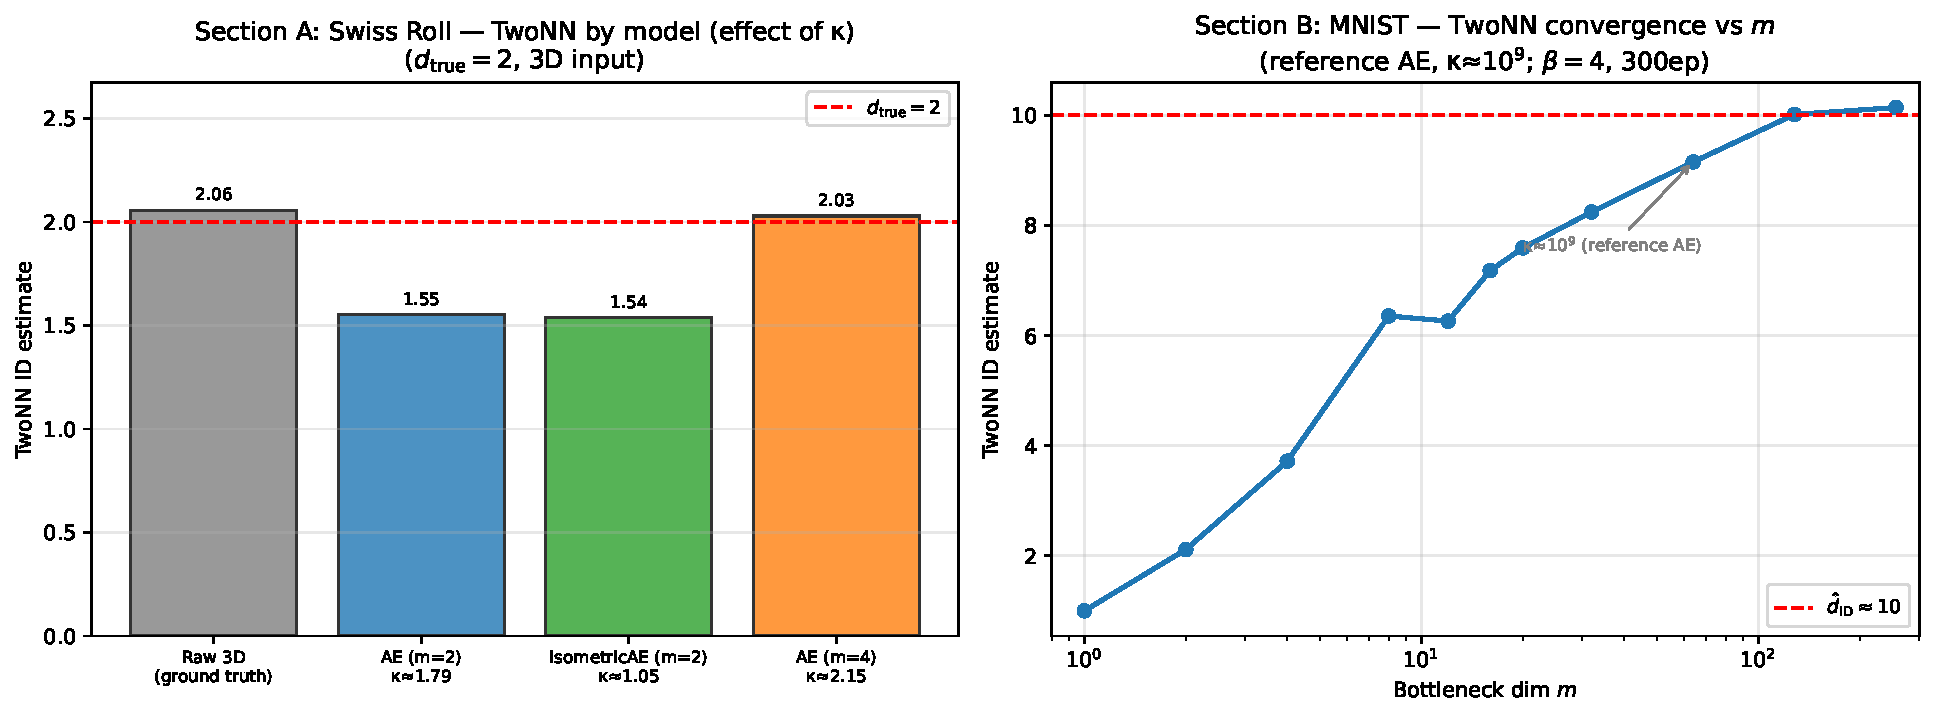
\includegraphics[width=0.95\linewidth]{results/figures/EP_twonn_stability.pdf}
  \caption{Exp-Stab/Exp-Geom: (Left) TwoNN ID on Swiss Roll --- AE and IsometricAE both underestimate at $m=d_\mathrm{true}$; TwoNN recovers at $m=4>d_\mathrm{true}$. (Right) MNIST AE $m$-sweep: TwoNN stabilizes at $m \geq 48$ despite $\kap$ jumping to $37.0$ at $m=128$. Detailed tables in Appendix D.}
  \label{fig:ep}
\end{figure}}{}

\subsection{MNIST：有効表現次元の読み取り（主実験，RQ1・RQ2）}\label{sec:exp_mnist}

MNIST データセットを用いて，提案フレームワークの実データへの適用を検証する（主実験）．
MNIST は「実データであり，$\dtrue$は未知であるが$\hat{d}_\mathrm{ID}$を推定できる」
という意味で，フレームワークの現実的な評価環境を提供する．

\subsubsection{AE による内在次元の推定（実験 Exp-Mnist-Base-AE）}

MNIST AE（300 エポック）の結果を表\ref{tab:e4_ae}に示す．

\begin{table}[H]
\centering
\caption{Exp-Mnist-Base: MNIST AE results (300 epochs, $n_\mathrm{train}=20{,}000$).}
\label{tab:e4_ae}
\small
\begin{tabular}{rcccc}
\toprule
$m$ & MSE & TwoNN ID & MLE ID & CKA \\
\midrule
1   & 0.0437 & 1.02  & 1.15  & 0.102 \\
4   & 0.0292 & 3.86  & 4.29  & 0.575 \\
8   & 0.0191 & 6.08  & 6.70  & 0.725 \\
16  & 0.0121 & 7.96  & 8.61  & 0.812 \\
32  & 0.0087 & 8.84  & 9.89  & 0.875 \\
64  & 0.0062 & 9.54  & 11.26 & 0.908 \\
128 & 0.0061 & 9.84  & 11.45 & 0.921 \\
256 & 0.0057 & \textbf{10.02} & \textbf{11.85} & 0.953 \\
\bottomrule
\end{tabular}
\end{table}

$m \geq 64$で TwoNN ID（9.54〜10.02）と MLE ID（11.26〜11.85）が収束し，
MNIST の実効内在次元が概ね$\hat{d}_\mathrm{ID} \approx 10$〜12 の範囲にあることを示す．

\textbf{線形 PCA との比較}：
MNIST（$n = 20{,}000$）に PCA を適用すると，累積寄与率 80\% に 43 次元，
90\% に 86 次元が必要である．
AE（TwoNN $\approx 10$）の推定値と比較して 4〜8 倍大きく，
MNIST の非線形な多様体構造を示している（図\ref{fig:e4_dualaxis}参照）．

\subsubsection{VAE の AU Dynamics と$\mknee$（実験 Exp-Mnist-Base-VAE）}

MNIST VAE（$\beta = 4$，300 エポック）の AU パターンを表\ref{tab:e4_vae}および
図\ref{fig:e4_dualaxis}に示す．

\begin{table}[H]
\centering
\caption{Exp-Mnist-Base: MNIST VAE ($\beta=4$) results (300 epochs). AU increase rate slows at $m=12$ ($\mknee=12$).}
\label{tab:e4_vae}
\small
\begin{tabular}{rcccc}
\toprule
$m$ & MSE & AU & TwoNN ID & $r(m)$の変化 \\
\midrule
1   & 0.0464 & 1  & 1.00 & --- \\
4   & 0.0275 & 4  & 3.72 & 正常増加 \\
8   & 0.0186 & 8  & 6.36 & 正常増加 \\
\textbf{12} & 0.0184 & \textbf{8}  & 6.26 & \textbf{急落} $\leftarrow \mknee = 12$ \\
16  & 0.0148 & 11 & 7.18 & 低 \\
20  & 0.0134 & 13 & 7.59 & 低 \\
32  & 0.0121 & 15 & 8.25 & 低 \\
64  & 0.0103 & 29 & 9.16 & 緩やか \\
128 & 0.0085 & 26 & 10.02 & 緩やか \\
256 & 0.0072 & 36 & 10.14 & 緩やか \\
\bottomrule
\end{tabular}
\end{table}

$m = 12$で AU $= 8$（前の$m = 8$と同じ）となり，AU 増加率$r(m)$が急落する（$r(12) \approx 0$）．
$\tau_{\mathrm{knee}} = 0.25$の閾値をトリガーし，$\mknee = 12$と観測される．

\textbf{注意}：この値は単一シード（seed 42）・特定の拡張グリッド（$m \in \{1,4,8,\ldots,256\}$）
での予備的観察であり，後続の多シード実験（§\ref{sec:exp_multiseed}，§\ref{sec:exp_multiseed2}）で
同じ$m$・グリッドで再現しないことが判明した．
単一シード・拡張グリッド条件では TwoNN ID の範囲（$\approx 10$〜12）と近い値を示したが，
\textbf{本論文では密グリッド・独立初期化・複数シードに基づく Exp-Mnist-Dense-300 の
$\mknee = 10.3 \pm 0.9$ を主要な安定化結果として扱う}（§\ref{sec:exp_el}）．

\IfFileExists{results/figures/E4_mnist_dualaxis.pdf}{%
\begin{figure}[H]
\centering
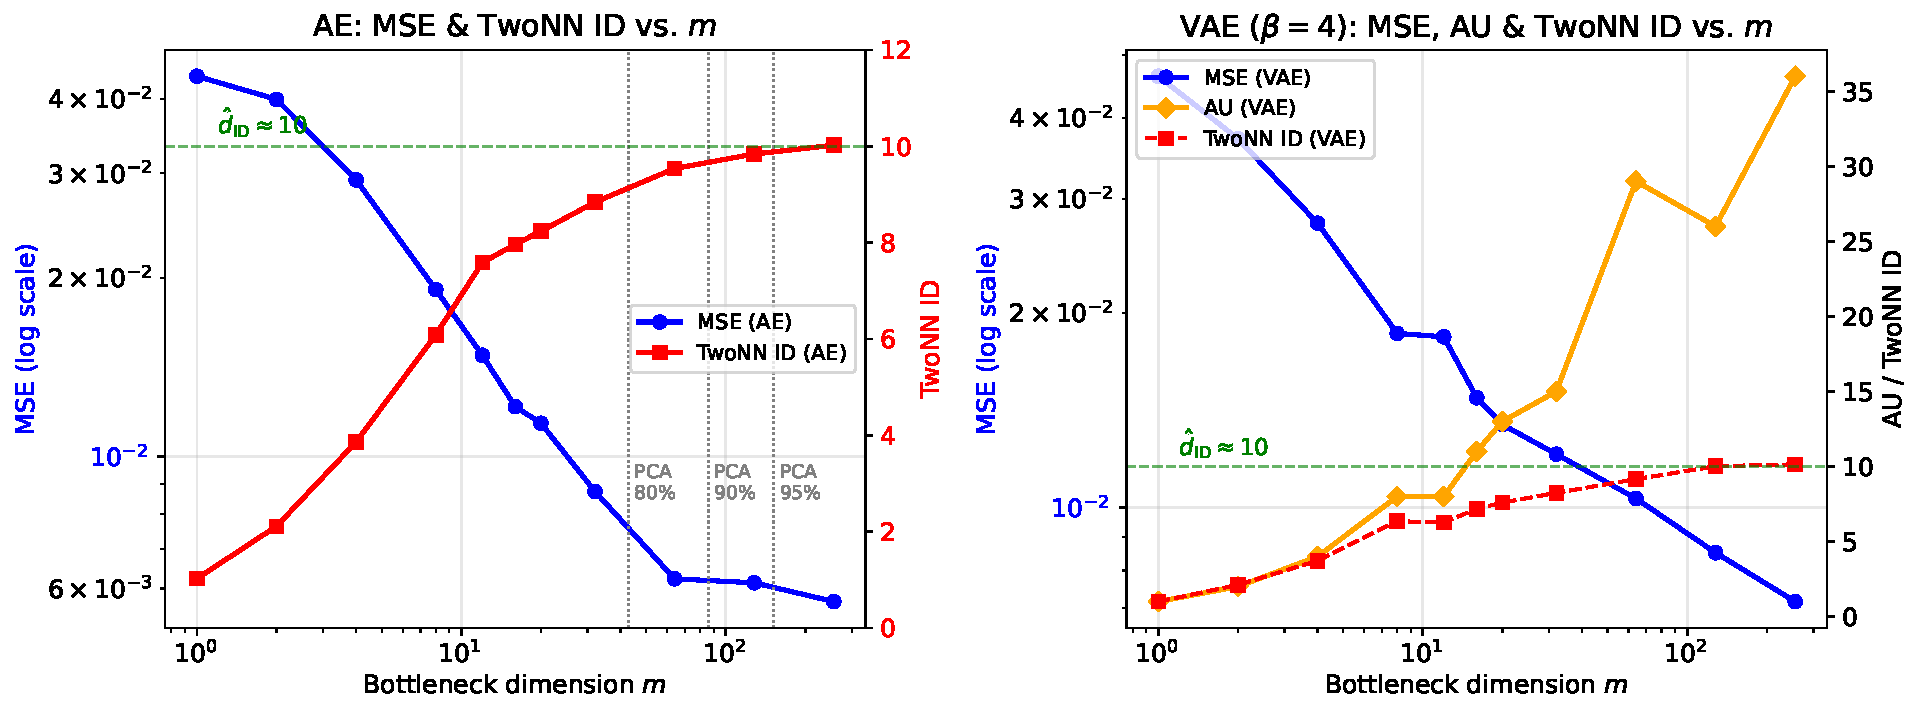
\includegraphics[width=0.95\linewidth]{results/figures/E4_mnist_dualaxis.pdf}
\caption{Exp-Mnist-Base: $m$-dependence of each indicator for MNIST (300 epochs). \textbf{Left (AE)}: MSE (log scale, left axis) and TwoNN ID (right axis). Vertical dotted lines correspond to PCA cumulative variance 80\% (43 dims), 90\% (86 dims), 95\% (152 dims); the difference from the nonlinear AE estimate (TwoNN $\approx 10$) is clear. \textbf{Right (VAE, $\beta=4$)}: MSE (log scale, left axis), AU (right axis), TwoNN ID (right axis, dashed). At $m = 12$ ($\mknee$), the AU increase rate drops sharply (arrow), indicating a heuristic slowdown point; the main stabilized result is $\mknee=10.3\pm0.9$ from Exp-Mnist-Dense-300 (§\ref{sec:exp_el}).}
\label{fig:e4_dualaxis}
\end{figure}}{}%

\subsubsection{既存指標との比較}\label{sec:exp_comparison}

提案指標$\mknee$を，他の代表的なボトルネック次元設計指標と比較する（表\ref{tab:method_comparison}）．

\begin{table}[H]
\centering
\caption{Comparison of bottleneck dimension estimates on MNIST.}
\label{tab:method_comparison}
\small
\begin{tabular}{p{3.8cm}cc p{4.8cm}}
\toprule
Method & Estimate & Source & Characteristics / Limitations \\
\midrule
PCA (80\% var.) & 43 & Exp-Mnist-Base-AE & Linear; overestimates nonlinear ID \\
PCA (90\% var.) & 86 & Exp-Mnist-Base-AE & Linear; larger overestimate \\
MSE elbow (AE) & $\approx16$--$20$ & Exp-Mnist-Base-AE & Intuitive; depends on smoothing \\
TwoNN ID (ref.\ AE) & $\approx10$--$12$ & Exp-Mnist-Base-AE & Nonlinear; subject to isometry bias \\
$\mknee$ (VAE, $\tau{=}0.25$) & 32--64* & Exp-Mnist-Multi & KL dynamics; grid/seed/init.-dependent \\
\midrule
\multicolumn{4}{p{13cm}}{\footnotesize *Multi-seed sparse-grid result (300ep, 3 seeds); a single preliminary run with an extended grid ($m\in\{1,\ldots,256\}$, seed 42) yielded $\mknee=12$, but this depends on random-state management and should be treated as a preliminary observation. Dense-grid result: $10.3\pm0.9$ (Exp-Mnist-Dense).} \\
\bottomrule
\end{tabular}
\end{table}

各手法の特徴：
PCA は線形手法であるため MNIST の非線形な多様体構造を反映できず，
AE（TwoNN $\approx 10$）の4倍以上の次元を要求する．
MSE エルボーは直感的だが，平滑な MSE 曲線（Exp-Mnist-Base 参照）では肘点の決定が曖昧になりやすい．
TwoNN は非線形 ID 推定として有効だが，参照 AE の等長性バイアスを伴う．
$\mknee$は KL ダイナミクスを直接観察する点でこれらと相補的な指標であるが，
$\tau$・$\beta$・$m$グリッドへの依存性があり，単独での利用よりも
他の指標と組み合わせた多指標アプローチでの使用が望ましい．

\subsubsection{多シード検証（実験 Exp-Mnist-Multi-150）}\label{sec:exp_multiseed}

$\mknee$の統計的信頼性を評価するため，
MNIST VAE（$\beta = 4$，150 エポック，$m \in \{4,8,12,16,20,32,64\}$）を
3つの乱数シード（42，123，777）で繰り返した（実験 Exp-Mnist-Multi-150；表\ref{tab:e4_multiseed}）．

\begin{table}[H]
\centering
\caption{Exp-Mnist-Multi-150: Mean$\pm$std of AU and TwoNN ID for 3 seeds (42, 123, 777) at 150 epochs ($\beta=4$). AU values are highly consistent across seeds, but $\mknee$ varies.}
\label{tab:e4_multiseed}
\small
\begin{tabular}{rccl}
\toprule
$m$ & AU (mean$\pm$std) & TwoNN ID (mean$\pm$std) & Note \\
\midrule
 4 & $4.0 \pm 0.0$ & $3.98 \pm 0.06$ & all dims active \\
 8 & $7.7 \pm 0.5$ & $6.37 \pm 0.41$ & \\
12 & $10.0 \pm 0.0$ & $7.35 \pm 0.19$ & \\
16 & $11.3 \pm 0.5$ & $7.66 \pm 0.18$ & \\
20 & $13.3 \pm 0.5$ & $8.31 \pm 0.18$ & \\
32 & $16.0 \pm 0.0$ & $8.92 \pm 0.14$ & \\
64 & $22.0 \pm 0.0$ & $9.94 \pm 0.08$ & $\hat{d}_\mathrm{ID} \approx 10$ に収束 \\
\midrule
\multicolumn{4}{l}{$\mknee$（$\tau=0.25$）：シード 42 = 64，シード 123 = 32，シード 777 = 64} \\
\multicolumn{4}{l}{平均$\mknee = 53 \pm 15$（150 エポック）；主結果は密グリッド・独立初期化の Exp-Mnist-Dense-300: $\mknee = 10.3 \pm 0.9$} \\
\bottomrule
\end{tabular}
\end{table}

\IfFileExists{results/figures/E4_multiseed.pdf}{%
\begin{figure}[H]
  \centering
  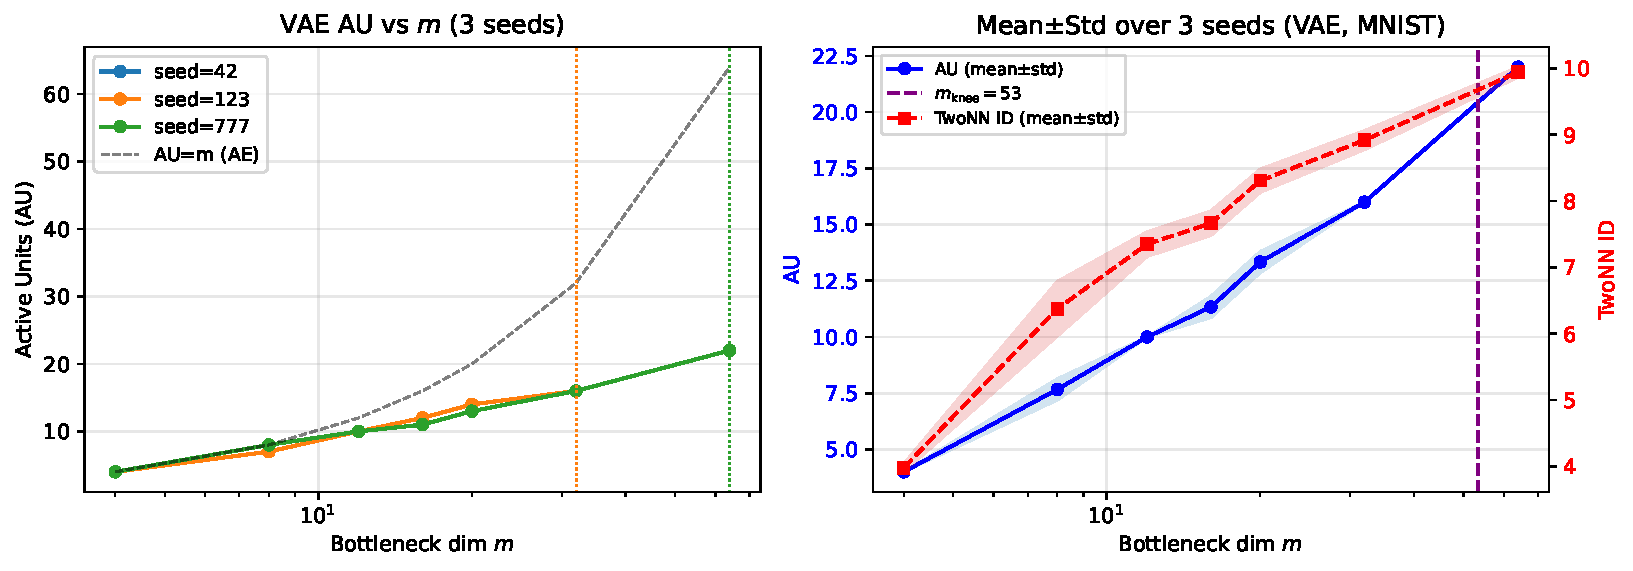
\includegraphics[width=0.9\linewidth]{results/figures/E4_multiseed.pdf}
  \caption{Exp-Mnist-Multi: AU patterns of MNIST VAE (3 seeds). Left: AU vs $m$ per seed (dotted lines: $\mknee$ per seed); Right: mean$\pm$std band. AU values are highly consistent across seeds, but $\mknee$ varies between 32 and 64.}
  \label{fig:e4_multiseed}
\end{figure}}{}

\textbf{主要知見}：
各$m$での AU 値は3シードにわたって高度に一致する（$\sigma \leq 0.5$；表\ref{tab:e4_multiseed}）．
TwoNN ID も$m = 64$で$9.94 \pm 0.08$と収束しており，$\hat{d}_\mathrm{ID} \approx 10$の推定は
シード不変であることを確認した．

一方，$\mknee$（$\tau = 0.25$）はシード 42 = 64，シード 123 = 32，シード 777 = 64 と変動した
（平均$53 \pm 15$）．
これは，AU 増加率$r(m)$が閾値 $\tau = 0.25$ に近い複数の$m$値で微妙に変動するためであり，
150 エポックの不完全収束下ではこの不安定性が増幅される．
なお，Exp-Mnist-Base 拡張実験（単一シード 42）では 300 エポックで$\mknee = 12$が得られたが，
後述の 300 エポック多シード実験（§\ref{sec:exp_multiseed2}）でも不安定性は残る（平均$43 \pm 15$）．
\textbf{150 エポック時点では収束不足の影響が重なっているが，
300 エポックに延長しても$\mknee$の数値的安定性が回復するわけではなく，
$m$グリッドと乱数シードへの依存が主因であることが判明した}（§\ref{sec:exp_multiseed2}）．
この知見は§\ref{sec:disc_limitation}で限界として記載した内容を定量的に裏付ける．

\subsubsection{300エポック多シード検証（実験 Exp-Mnist-Multi-300）}\label{sec:exp_multiseed2}

150 エポック実験での$\mknee$不安定性が収束不足によるものかを検証するため，
同条件（MNIST VAE，$\beta = 4$，$m \in \{4, 8, 12, 16, 20, 32, 64\}$）でエポック数を
300 に延長した実験（Exp-Mnist-Multi-300）を3シード（42，123，777）で実施した（表\ref{tab:e4_300ep_multiseed}）．

\begin{table}[H]
\centering
\caption{Exp-Mnist-Multi-300: Mean$\pm$std of AU and TwoNN ID for 3 seeds at 300 epochs ($\beta=4$). AU and TwoNN ID are highly consistent, but $\mknee$ still varies.}
\label{tab:e4_300ep_multiseed}
\small
\begin{tabular}{rccl}
\toprule
$m$ & AU (mean$\pm$std) & TwoNN ID (mean$\pm$std) & Note \\
\midrule
 4 & $4.0 \pm 0.0$ & $3.98 \pm 0.14$ & all dims active \\
 8 & $8.0 \pm 0.0$ & $6.67 \pm 0.15$ & \\
12 & $10.0 \pm 0.0$ & $7.41 \pm 0.06$ & \\
16 & $11.7 \pm 0.5$ & $7.95 \pm 0.21$ & AU still increasing \\
20 & $13.3 \pm 0.5$ & $8.37 \pm 0.14$ & \\
32 & $15.7 \pm 0.5$ & $9.07 \pm 0.10$ & \\
64 & $22.3 \pm 0.5$ & $10.03 \pm 0.12$ & converges to $\hat{d}_\mathrm{ID} \approx 10$ \\
\midrule
\multicolumn{4}{l}{$\mknee$（$\tau=0.25$）：シード 42 = 64，シード 123 = 32，シード 777 = 32} \\
\multicolumn{4}{l}{平均$\mknee = 43 \pm 15$（300 エポック）} \\
\bottomrule
\end{tabular}
\end{table}

\IfFileExists{results/figures/E4_300ep_multiseed.pdf}{%
\begin{figure}[H]
  \centering
  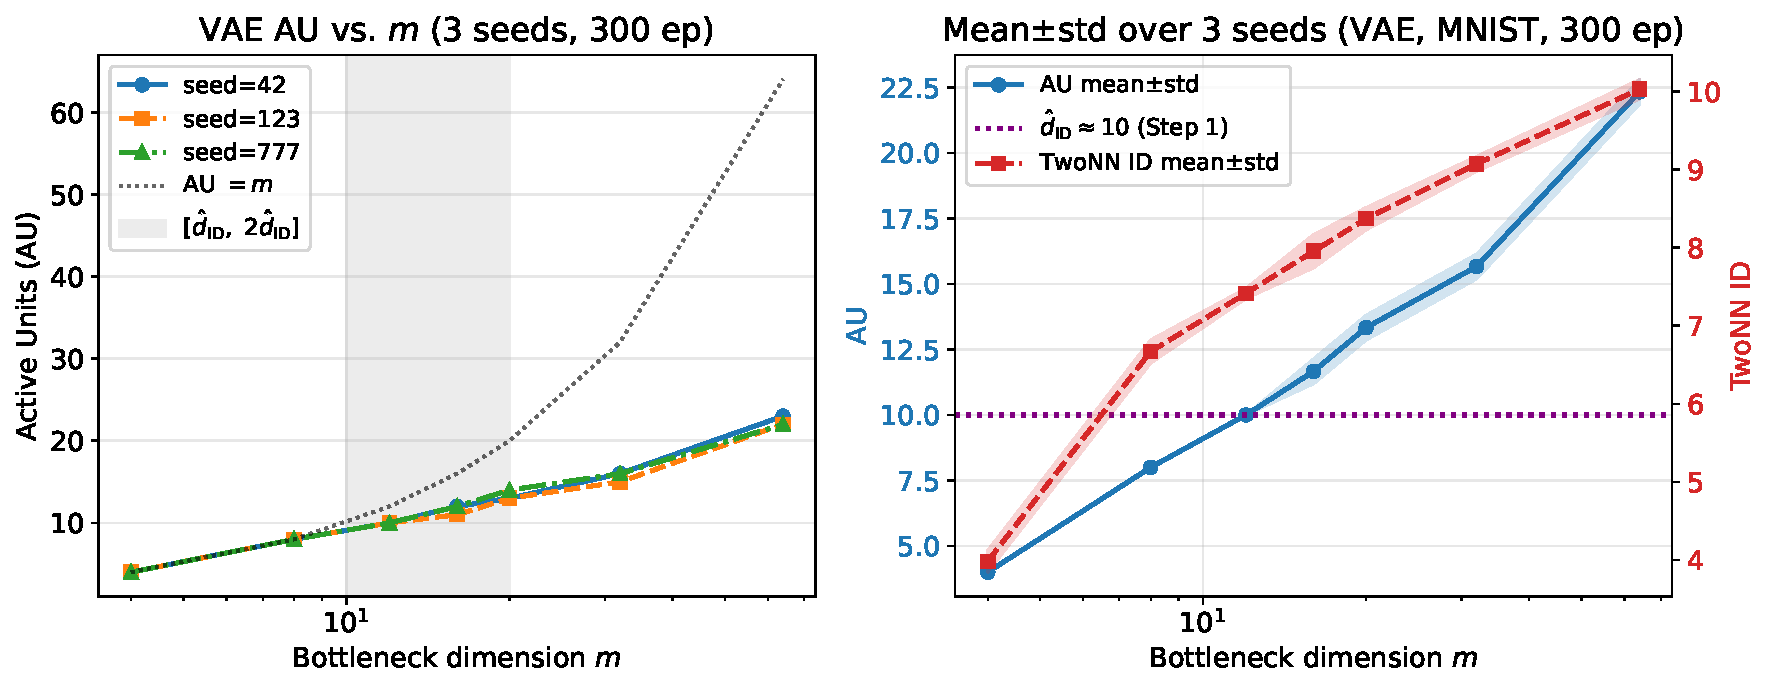
\includegraphics[width=0.9\linewidth]{results/figures/E4_300ep_multiseed.pdf}
  \caption{Exp-Mnist-Multi: AU patterns of MNIST VAE (3 seeds, 300 epochs). Left: AU vs $m$ per seed (dotted lines: $\mknee$); Right: mean$\pm$std band. AU and TwoNN ID bands are very narrow, but $\mknee$ varies between 32 and 64 across seeds.}
  \label{fig:e4_300ep_multiseed}
\end{figure}}{}

\textbf{主要知見}：
AU 値（表\ref{tab:e4_300ep_multiseed}）は300エポックでも3シード間で高度に一致し
（$\sigma \leq 0.5$），TwoNN ID も$m = 64$で$10.03 \pm 0.12$と安定している．
これらの定量的指標はシード・収束度に対してロバストであることを確認した．

一方，$\mknee$は 300 エポックの完全収束下でもシード間で 32〜64 に変動した
（平均$43 \pm 15$）．
これは，Exp-Mnist-Multi-150（：$\mknee = 32$〜$64$）と本質的に同一の変動範囲であり，
エポック数を 300 に延長しても$\mknee$の不安定性は解消されなかった．

なお，Exp-Mnist-Base 拡張実験での$\mknee = 12$はグリッド設計と初期化経路に依存する予備的観察であり，
本論文では独立初期化・複数シード・密グリッド条件の Exp-Mnist-Dense-300 の
$\mknee = 10.3 \pm 0.9$ を主結果として採用する（実装の詳細は付録\ref{app:twonn_detail}）．
\textbf{$\mknee$は AU 増加曲線から導かれる探索的変化点であり，
その値は実験設定（グリッド・シード・初期化）に依存する．}

\subsubsection{線形理論―実験橋渡し（実験 Exp-Mnist-PCA，詳細は付録\ref{app:twonn_detail}）}\label{sec:exp_em}

MNIST PCA スペクトル（$\lambda_1=5.22, \ldots, \lambda_{10}=1.23$）と定理\ref{thm:linear_vae}を対照すると，
$\tau^2_\mathrm{eff} \approx 0.30$（逆算値）で$d^* \approx 10$となり観測 TwoNN ID と定性的に整合する．
線形設定では鋭い飽和転換が生じるが，非線形 VAE では勾配競合により滑らかな漸増曲線となるため，
$\mknee$の疎グリッドでの不安定性が理論的に裏付けられる（詳細な PCA スペクトル表・理論-実験比較表は付録\ref{app:twonn_detail}）．
Conv-VAE では非線形デコーダの強力な再構成能力により$\tau^2_\mathrm{eff}$がさらに小さくなり，
AU 飽和に必要な$m$が FC-VAE 比で大幅に増大する（§\ref{sec:disc_convvae}）．

\subsubsection{密グリッド×シード×エポック因子分離実験（実験 Exp-Mnist-Dense）}\label{sec:exp_el}

$\mknee$の不安定性がどの要因に起因するかを厳密に特定するため，
グリッド密度・エポック・シードの3要因を単離した実験を設計した．
Exp-Mnist-Base と Exp-Mnist-Multi では既にエポック因子（150ep vs. 300ep）とシード因子（3シード）が分離されている．
本実験 Exp-Mnist-Dense ではさらにグリッド密度因子を単離する：$m \in \{8,9,10,11,12,13,14,15,16,18,20,24,28,32,40,48,64\}$
（17点，隣接点間隔 1〜8）で300エポック・3シードで学習した．
密グリッドは特に$m = 8$〜16（推定 $\hat{d}_\mathrm{ID} \approx 10$ の前後）を 1 刻みでカバーする
（命題\ref{thm:mknee_instab}は理想化モデルに対する補助的上界であり，
間隔 1 の密グリッドで$\mknee$が$d^*$近傍に収まる可能性はあるが，非線形 VAE の AU 揺動により実際の誤差が上界を超えることもある）．

\begin{table}[H]
\centering
\caption{Exp-Mnist-Dense: Comparison of $\mknee$ between dense and sparse grids ($\tau=0.25$, MNIST FC-VAE, $\beta=4$). Consistent with the grid-sensitivity bound of Proposition \ref{thm:mknee_instab}.}
\label{tab:el_mknee}
\small
\begin{tabular}{lccccc}
\toprule
Condition & Max.\ grid interval & seed=42 & seed=123 & seed=777 & Mean$\pm$std \\
\midrule
Sparse grid, 150ep (Exp-Mnist-Multi-150) & 32 & 64 & 32 & 64 & $53 \pm 15$ \\
Sparse grid, 300ep (Exp-Mnist-Multi-300) & 32 & 64 & 32 & 32 & $43 \pm 15$ \\
Dense grid, 300ep (Exp-Mnist-Dense-300) & 8 (step 1 for 8--16) & 11 & 9 & 11 & $10.3 \pm 0.9$ \\
\bottomrule
\end{tabular}
\end{table}

\begin{table}[H]
\centering
\caption{Exp-Mnist-Dense: AU$(m)$ for dense grid (seed=42, 300ep, representative values).}
\label{tab:el_au}
\small
\begin{tabular}{rcccccccc}
\toprule
$m$ & 8 & 9 & 10 & 11 & 12 & 13 & 14 & 15 \\
\midrule
AU & 8 & 9 & 10 & 10 & 10 & 10 & 12 & 11 \\
\midrule
$m$ & 16 & 18 & 20 & 24 & 28 & 32 & 48 & 64 \\
\midrule
AU & 14 & 13 & 15 & 14 & 15 & 15 & 19 & 21 \\
\bottomrule
\end{tabular}
\end{table}

\IfFileExists{results/figures/EL_dense_grid_mknee.pdf}{%
\begin{figure}[H]
  \centering
  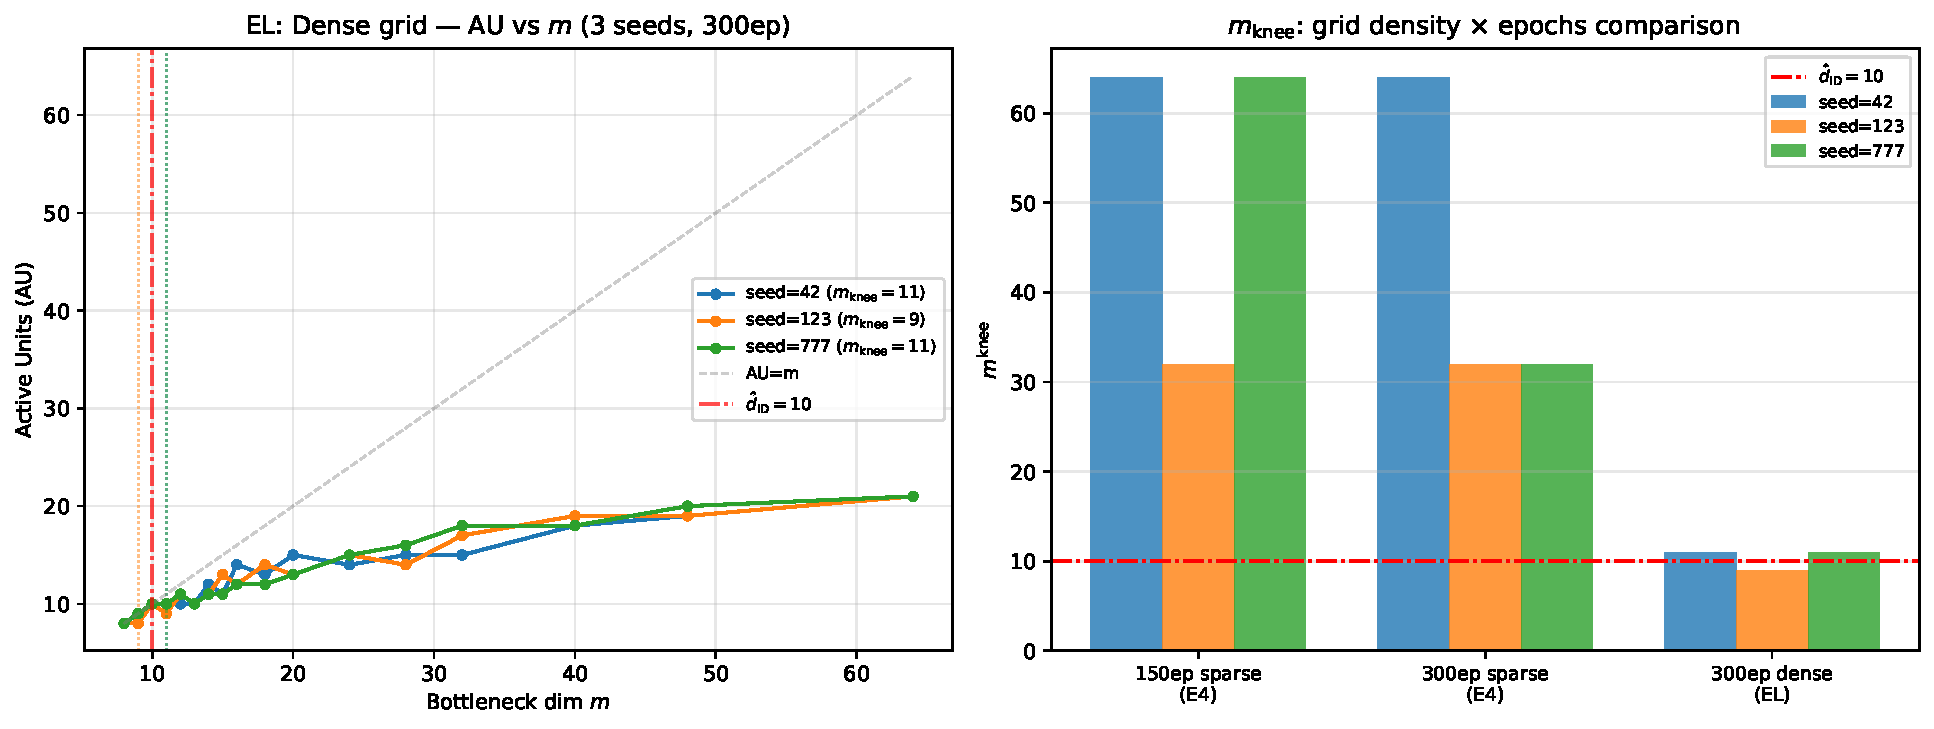
\includegraphics[width=0.95\linewidth]{results/figures/EL_dense_grid_mknee.pdf}
  \caption{Exp-Mnist-Dense: (Left) Dense-grid AU vs $m$ (3 seeds). (Right) Comparison by grid density $\times$ epochs. $\mknee$ variation in the dense grid can be assessed by the upper bound of Proposition~\ref{thm:mknee_instab} (maximum grid interval).}
  \label{fig:el}
\end{figure}}{}

\textbf{Exp-Mnist-Dense 実験の意義}：
表\ref{tab:el_mknee}の3行比較により，3要因（グリッド密度・エポック・シード）が定量的に単離される：
\begin{itemize}
  \item \textbf{エポック因子}：疎グリッド 150ep → 300ep（$\mknee$: $53\pm15$ → $43\pm15$）—— エポック増加で若干安定するが，主因ではない
  \item \textbf{シード因子}：同一条件の3シード間での変動（$\sigma = 15$）—— 初期化による最適化経路の差が影響するが，疎グリッドと共存する二次的因子
  \item \textbf{グリッド密度因子（主要因の一つ）}：密グリッド（Exp-Mnist-Dense）では$\mknee = 10.3 \pm 0.9$（seed=[11,9,11]）—— 疎グリッド$43\pm15$から劇的に改善し，推定$\hat{d}_\mathrm{ID} \approx 10$と整合する
\end{itemize}

\noindent
\textbf{命題\ref{thm:mknee_instab}との整合性}：
Exp-Mnist-Dense 実験は命題\ref{thm:mknee_instab}が示唆するグリッド感度と定性的に整合する．
密グリッドで$m = 8$〜16 の間隔を 1 に削減した結果，
$\mknee \in \{9, 11\}$（3シード）となり，$d^* \approx 10$との乖離が 1 以内に収まった
（上界 = 最大グリッド間隔 = 8（$m > 16$の区間）だが，検出は間隔 1 の密な区間で起こる）．
ただし，命題\ref{thm:mknee_instab}は理想化単調飽和モデルを仮定しており，
非線形 VAE の AU 揺動により実際の誤差は上界を超えうる点に注意が必要である．
これらの観察は，$\mknee$の不安定性にグリッド設計が寄与するという解釈を定性的に支持する．
ただし，シード因子も二次的に寄与することは本実験でも確認されており（疎グリッドでの3シード変動；§\ref{sec:exp_multiseed2}），
また非線形最適化での飽和の滑らかさにより，命題\ref{thm:mknee_instab}の上界を超えた誤差が生じうる点にも留意が必要である．

\noindent
\textbf{$\tau$法と二階差分法の比較}：
$\mknee$の検出には，本稿で採用している一階差分比率法（$\tau = 0.25$）のほかに，
AU$(m)$曲線の曲率が最大となる点を求める\textbf{二階差分法}（\ref{app:tau_knee}）がある．
Exp-Mnist-Dense 密グリッドデータでの比較結果を表\ref{tab:el_knee_compare}に示す．

\begin{table}[H]
\centering
\caption{Exp-Mnist-Dense: Comparison of $\tau$-method ($\tau=0.25$) and second-difference method (d2) for $\mknee$ detection (dense grid, 300ep, 3 seeds).}
\label{tab:el_knee_compare}
\small
\begin{tabular}{lcccc}
\toprule
Method & seed=42 & seed=123 & seed=777 & Mean$\pm$std \\
\midrule
$\tau$-method ($\tau=0.25$) & 11 & 9  & 11 & $10.3 \pm 0.9$ \\
Second-difference method (d2) & 15 & 28 & 12 & $18.3 \pm 6.8$ \\
\midrule
\multicolumn{5}{l}{Reference: $\hat{d}_\mathrm{ID} \approx 10$ (TwoNN, $m=64$, 3-seed mean)} \\
\bottomrule
\end{tabular}
\end{table}

$\tau$法は平均$10.3 \pm 0.9$と$\hat{d}_\mathrm{ID} \approx 10$に整合し，シード間変動が小さい．
一方，d2 法は AU$(m)$の離散的ノイズに敏感で，seed=123 では$\mknee = 28$と大きく外れた
（AU 曲線の遷移域で AU が 8→10→9→11→10→11→13 と揺動し，二階差分の最大値点が乱れる）．
したがって，\textbf{密グリッド条件での$\mknee$検出には$\tau$法の方が安定}であり，
d2 法は大域的な「肘点」候補を探す補助手段として位置づける（\ref{app:tau_knee}参照）．

なお，MNIST VAE の$\AUsat = 36$（$m=256$）が$\hat{d}_\mathrm{ID} \approx 10$〜12 を大幅に超える点（Manifold Entanglement 仮説）と，
学習ダイナミクスの2フェーズパターン（Exp-Mnist-Dyn）は，いずれも単一シード・予備的観察であり，
多シード検証は今後の課題として残す（§\ref{sec:disc_incidental}参照）．

\subsection{Fashion-MNIST への適用（実験 Exp-Fashion，単一シード）}\label{sec:exp_fashion}

Fashion-MNIST（衣類 10 クラス，28×28）に対して MNIST と同一のアーキテクチャ・設定を適用し，
フレームワークの異種実データへの適用性を確認する．
\textbf{注意}：本実験は単一シード（seed 42）での確認であり，
MNIST（3シード）と同水準の再現性の主張はしない．Fashion-MNIST 3シード実験は今後の課題である．

\begin{table}[H]
\centering
\caption{Exp-Fashion: Fashion-MNIST AE and VAE results (100 epochs, $n_\mathrm{train}=10{,}000$, representative $m$ values).}
\label{tab:ef}
\small
\begin{tabular}{rcccrcc}
\toprule
\multicolumn{3}{c}{AE} & \phantom{xx} & \multicolumn{3}{c}{VAE（$\beta=4$）} \\
\cmidrule{1-3}\cmidrule{5-7}
$m$ & MSE & TwoNN ID && $m$ & MSE & AU \\
\midrule
 4  & 0.01831 & 3.90 && 4  & 0.01955 & 4  \\
 8  & 0.01389 & 5.86 && 8  & 0.01721 & 6  \\
12  & 0.01230 & 7.58 && 12 & 0.01597 & 6  \\
16  & 0.01138 & 8.11 && 16 & 0.01570 & 7  \\
20  & 0.01077 & 8.45 && 20 & 0.01471 & 8  \\
32  & 0.01010 & 8.99 && 32 & 0.01418 & 9  \\
64  & 0.00981 & 9.39 && 64 & 0.01318 & 11 \\
256 & 0.01009 & 9.42 && 256& 0.01193 & 25 \\
\bottomrule
\end{tabular}
\end{table}

\begin{figure}[t]
  \centering
  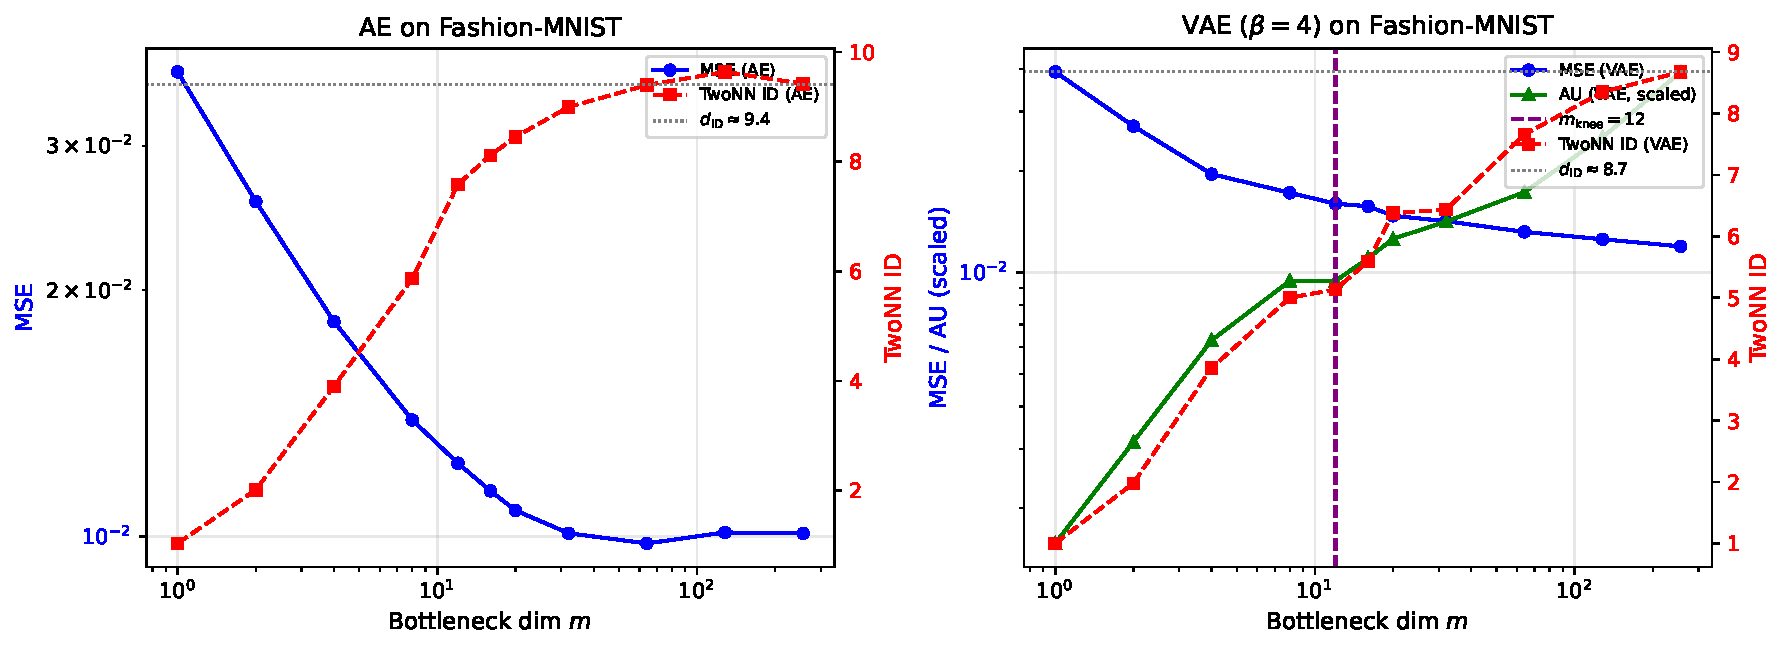
\includegraphics[width=0.9\linewidth]{results/figures/EF_fashion_mnist_dualaxis.pdf}
  \caption{Exp-Fashion: $m$-dependence of MSE, AU, and TwoNN ID for Fashion-MNIST AE (left) and VAE (right) (100 epochs). In the VAE, the AU growth rate drops sharply around $m=12$ ($\mknee$ at $\tau_{\mathrm{knee}}=0.25$), and TwoNN ID asymptotically converges to $\approx 9.4$ (AE) and $\approx 8.7$ (VAE) at $m \geq 32$.}
  \label{fig:ef}
\end{figure}

実験 Exp-Fashion の結果（表\ref{tab:ef}，図\ref{fig:ef}）から，以下の知見が得られる．
AE では pseudo-AU $= m$（全潜在座標が実質的に活性）かつ TwoNN ID が $m \geq 32$ で $\approx 9.4$ に収束し，
Fashion-MNIST の$\hat{d}_\mathrm{ID} \approx 9$〜10 が示唆される．
VAE（$\beta=4$，単一シード）では$\mknee = 12$（$\tau_{\mathrm{knee}} = 0.25$）が観測されたが，
これは単一シードの探索的観察であり，MNIST での多シード疎グリッド結果（$\mknee = 43 \pm 15$）と
同水準の再現性は保証されない点に注意が必要である．
AU は$m = 256$ でも 25 にとどまり（MNIST の 36 と異なり），
Fashion-MNIST が MNIST より高い圧縮難度をもつ可能性を示す．
TwoNN ID の推定値（$\approx 9$〜10）は MNIST（$\approx 10$〜12）より小さく，
衣類の方が手書き数字より局所的な自由度が少ないという直感と整合する．

\subsection{畳み込みアーキテクチャへの拡張（実験 Exp-Conv-AE）}\label{sec:exp_conv}

全結合型に限定した場合の一般化可能性への懸念に対し，
畳み込み型 AE/VAE（Conv-AE/VAE）を MNIST に適用した実験（実験 Exp-Conv-AE）を実施した．

\textbf{Conv-AE/VAE アーキテクチャ}：
\begin{itemize}
  \item エンコーダ：Conv($1\to32$, $k=3$, stride$=2$) $\to$ Conv($32\to64$, $k=3$, stride$=2$)
        $\to$ FC($3136\to m$)（VAE では$\to \mu, \log\sigma^2$）
  \item デコーダ：FC($m\to3136$) $\to$ ConvT($64\to32$, $k=4$, stride$=2$) $\to$
        ConvT($32\to1$, $k=4$, stride$=2$) $\to$ Sigmoid
  \item $n_{\mathrm{train}} = 20{,}000$，100 エポック，$m \in \{4, 8, 12, 16, 20, 32, 64\}$，seed 42
\end{itemize}

\begin{table}[H]
\centering
\caption{Exp-Conv-AE: MNIST Conv-AE and Conv-VAE ($\beta=4$) results (100 epochs, seed=42).}
\label{tab:eg}
\small
\begin{tabular}{rcc|rcc}
\toprule
\multicolumn{3}{c|}{Conv-AE} & \multicolumn{3}{c}{Conv-VAE ($\beta=4$)} \\
$m$ & MSE & TwoNN ID & $m$ & MSE & AU \\
\midrule
 4  & 0.0311 & 4.18  &  4  & 0.0331 &  4 \\
 8  & 0.0174 & 6.59  &  8  & 0.0197 &  8 \\
12  & 0.0113 & 7.80  & 12  & 0.0140 & 12 \\
16  & 0.0081 & 8.69  & 16  & 0.0109 & 16 \\
20  & 0.0069 & 9.03  & 20  & 0.0097 & 20 \\
32  & 0.0042 & 10.06 & 32  & 0.0070 & 32 \\
64  & 0.0020 & 11.29 & 64  & 0.0049 & 63 \\
\bottomrule
\end{tabular}
\end{table}

\IfFileExists{results/figures/EG_conv_mnist.pdf}{%
\begin{figure}[H]
  \centering
  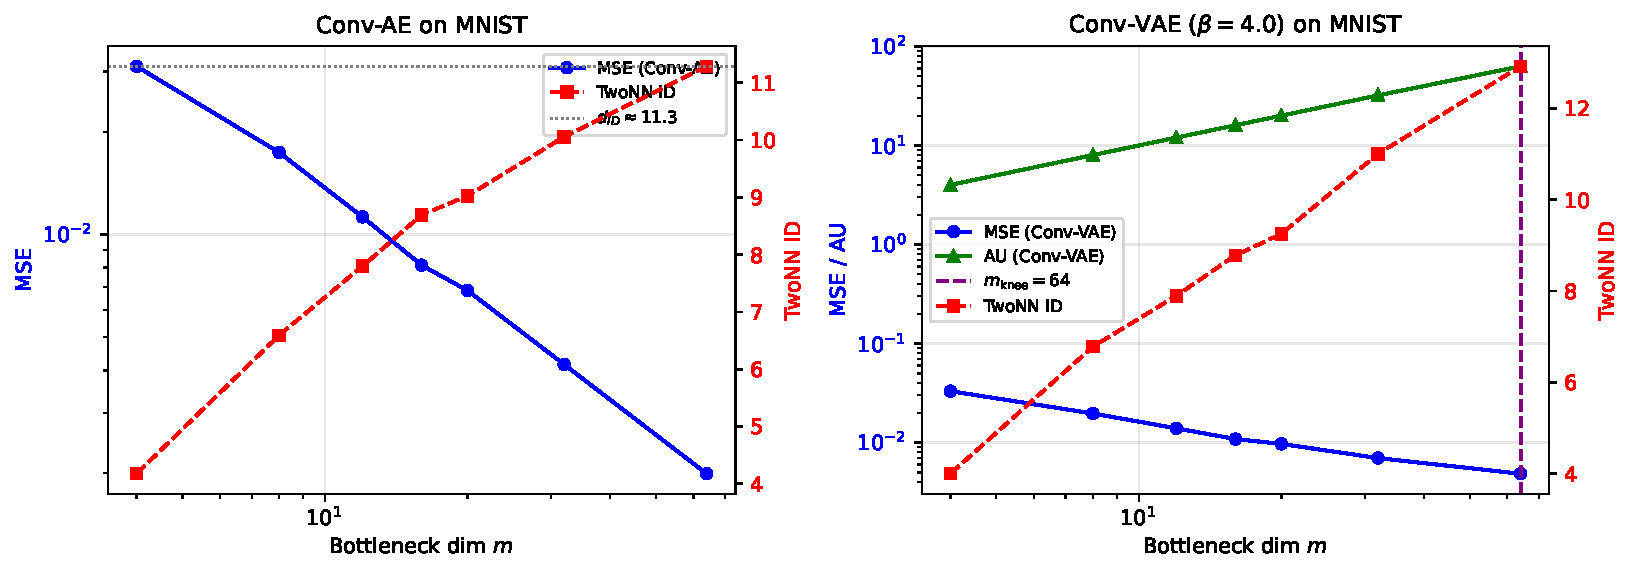
\includegraphics[width=0.9\linewidth]{results/figures/EG_conv_mnist.pdf}
  \caption{Exp-Conv-AE: $m$-dependence of MSE, AU, and TwoNN ID for MNIST Conv-AE (left) and Conv-VAE (right) (100 epochs). Conv-AE confirms AU$=m$ (all dims active) with TwoNN ID converging to $\approx 11$ at $m \geq 32$. Conv-VAE shows AU$\approx m$ (no saturation due to insufficient convergence at 100 epochs).}
  \label{fig:eg}
\end{figure}}{}

実験 Exp-Conv-AE の結果（表\ref{tab:eg}）から以下の知見が得られる．

\textbf{Conv-AE の TwoNN ID}：$m = 64$で TwoNN ID $= 11.29$に収束し，
FC-AE の推定値（$\approx 10$）と整合する（誤差$\approx 10\%$以内）．
アーキテクチャ（全結合 vs 畳み込み）によらず，TwoNN による ID 推定値が一貫することを確認した
（本研究条件下での経験的観測）．

\textbf{Conv-VAE の収束感度}：$m \leq 32$では AU $= m$（飽和なし），$m = 64$で AU $= 63$であり，
100 エポックでは KL 正則化による次元抑制が十分に機能していない．
これは FC-VAE での 150 エポック実験（Exp-Mnist-Multi：AU$\approx m$）と同様であり，
\textbf{Conv-VAE における$\mknee$の信頼ある検出にも，より多くのエポック数が必要}であることを示す．

\subsubsection{Conv-VAE での AU 飽和遅延：固定$\beta$・KL アニーリング比較（実験 Exp-Conv-Fix・Exp-Conv-Ann）}
\label{sec:exp_conv_300ep}

Exp-Conv-AE の収束不足を受け，300ep・3シード（Exp-Conv-Fix）および KL サイクリックアニーリング（Exp-Conv-Ann）で検証した
（表\ref{tab:eh_conv_vae}）．

\begin{table}[H]
\centering
\caption{Exp-Conv-Fix and Exp-Conv-Ann: Comparison of AU for MNIST Conv-VAE (300ep, mean$\pm$std over 3 seeds). FC-VAE (Exp-Mnist-Multi) saturates at $m=32$ (AU$=15.7$), while Conv-VAE shows AU$=m$ (no saturation) under both fixed-$\beta$ and annealing at $m \leq 32$.}
\label{tab:eh_conv_vae}
\small
\begin{tabular}{r ccc cc}
\toprule
 & \multicolumn{2}{c}{Conv-VAE fixed-$\beta$ (Exp-Conv-Fix)} & \multicolumn{1}{c}{Conv-VAE annealing (Exp-Conv-Ann)} & \multicolumn{2}{c}{FC-VAE (Exp-Mnist-Base, 300ep)} \\
$m$ & AU & TwoNN ID & AU & AU & TwoNN ID \\
\midrule
 4 & $4.0\pm0.0$ & $3.97\pm0.08$ & $4.0\pm0.0$ & $4.0$ & $3.98$ \\
12 & $12.0\pm0.0$ & $8.14\pm0.09$ & $12.0\pm0.0$ & $10.0$ & $7.41$ \\
32 & $32.0\pm0.0$ & $11.43\pm0.08$ & $32.0\pm0.0$ & $15.7$ & $9.07$ \\
64 & $54.3\pm0.5$ & $13.10\pm0.05$ & $64.0\pm0.0$ & $22.3$ & $10.03$ \\
\midrule
\multicolumn{6}{l}{$\mknee$：Conv-VAE（両条件）全シード=64（グリッド上限）；FC-VAE=$43\pm15$（32〜64）} \\
\bottomrule
\end{tabular}
\end{table}

Conv-VAE は固定$\beta=4$・サイクリックアニーリングいずれでも$m \leq 32$で AU$=m$（飽和なし）であり，
FC-VAE との乖離が明確である（§\ref{sec:disc_convvae}で理論的考察）．
AU$\approx m$は「KL 正則化が未機能」のシグナルであり，この状態では TwoNN ID も膨張する
（Conv-VAE $m=64$: $13.10$，FC-VAE: $10.03$）．
\textbf{$m \leq 64$のグリッドでは AU 飽和の観察が不可能}であり，$m$ 範囲の拡張が必要である．

%% ===================================================================
\subsection{Conv-VAE 拡張$m$グリッド実験（実験 Exp-Conv-M256・Exp-Conv-M512）}\label{sec:exp_en}

Exp-Conv-Fix・Exp-Conv-Ann（§\ref{sec:exp_conv_300ep}）で$m \leq 64$では AU 飽和が観測されなかったことを受け，
$m$グリッドを 256（実験 Exp-Conv-M256）および 512（実験 Exp-Conv-M512）まで拡張した．
§\ref{sec:disc_convvae}で論じる$\tau^2_\mathrm{eff}$の低下仮説のもとでは，
Conv-VAE の$d^*(\beta)$は FC-VAE（$\approx 10$）より大幅に大きいため，
$m>64$の領域で AU 増加の鈍化が現れると予測される．

\textbf{実験設定}（Exp-Conv-M256）：
Exp-Conv-Ann と同一の Conv-VAE アーキテクチャ（$28\times28$ MNIST，2層 Conv エンコーダ・
2層 ConvTranspose デコーダ，KL サイクリックアニーリング$\beta_\mathrm{max}=4$，3サイクル，
150 エポック，seeds$\in\{42,123,777\}$）を用い，
$m \in \{4, 8, 16, 32, 64, 96, 128, 192, 256\}$（9点）を検証した．

\begin{table}[H]
\centering
\caption{Exp-Conv-M256: Conv-VAE extended $m$ grid (KL annealing, 150 epochs, mean$\pm$std, 3 seeds). AU$=m$ for $m \leq 64$; AU$<m$ begins at $m \geq 96$. FC-VAE reference (Exp-Mnist-Base, 300ep, $m=64$): AU$=22.3\pm0.5$.}
\label{tab:en}
\small
\begin{tabular}{rccc}
\toprule
$m$ & AU (mean$\pm$std) & TwoNN ID (mean$\pm$std) & Note \\
\midrule
  4 & $4.0\pm0.0$   & $3.84\pm0.11$ & all dims active \\
  8 & $8.0\pm0.0$   & $6.64\pm0.11$ & \\
 16 & $16.0\pm0.0$  & $8.76\pm0.05$ & \\
 32 & $32.0\pm0.0$  & $10.46\pm0.13$ & \\
 64 & $64.0\pm0.0$  & $13.29\pm0.12$ & same as Exp-Conv-Ann (no saturation) \\
 96 & $\mathbf{90.7\pm1.2}$  & $14.30\pm0.22$ & \textbf{AU$<m$ onset} (FC-VAE $\hat{d}_\mathrm{ID} \approx 9\times$) \\
128 & $111.7\pm2.6$ & $14.69\pm0.13$ & \\
192 & $159.0\pm4.3$ & $15.89\pm0.27$ & \\
256 & $241.3\pm2.9$ & $16.58\pm0.16$ & \\
\midrule
\multicolumn{4}{l}{$\mknee$（$\tau=0.25$）：全シード=256（検証範囲内に knee なし）} \\
\multicolumn{4}{l}{FC-VAE reference (Exp-Mnist-Base, 300ep, $m=64$): AU$=22.3\pm0.5$, TwoNN ID$=10.03\pm0.12$} \\
\bottomrule
\end{tabular}
\end{table}

\IfFileExists{results/figures/EN_conv_vae_extended_m.pdf}{%
\begin{figure}[H]
  \centering
  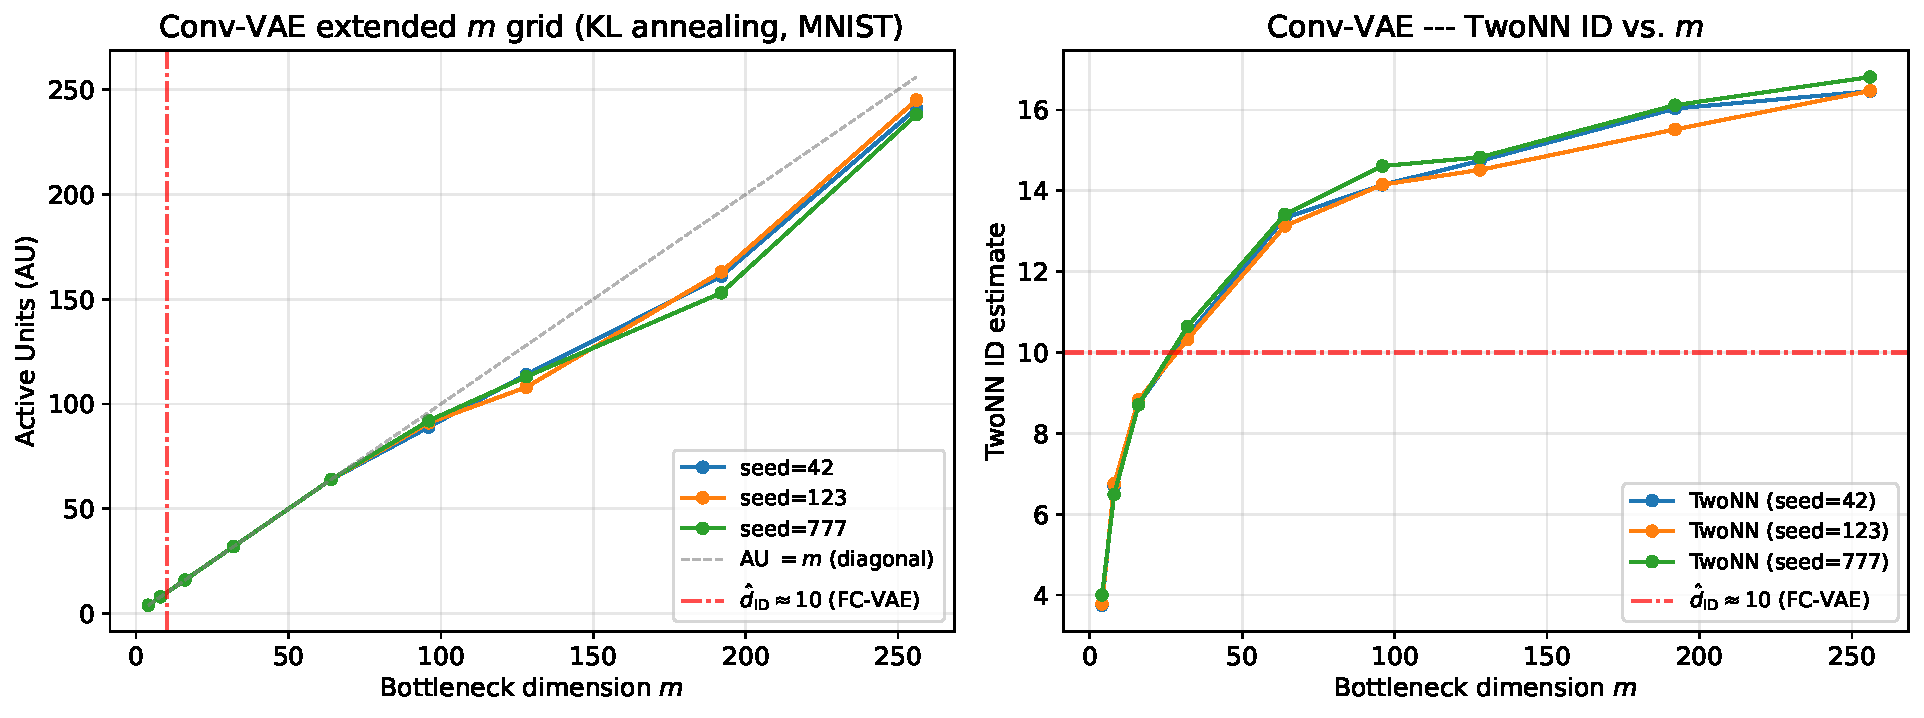
\includegraphics[width=0.95\linewidth]{results/figures/EN_conv_vae_extended_m.pdf}
  \caption{Exp-Conv-M256: Conv-VAE extended $m$ grid ($m\in[4,256]$, KL annealing, 3 seeds). AU vs $m$ (left) and TwoNN ID vs $m$ (right). Diagonal line (AU$=m$) and FC-VAE reference $\hat{d}_\mathrm{ID} \approx 10$ (red) are shown. AU$=m$ continues at $m \leq 64$ but deviates from the diagonal at $m \geq 96$, confirming qualitative water-filling behavior in Conv-VAE.}
  \label{fig:en}
\end{figure}}{}

\textbf{実験 Exp-Conv-M256 の主要知見}：
$m \leq 64$では AU$=m$が全3シードで一致し，FC-VAE（$m=64$: AU$=22.3$）との対比が際立つ．
$m = 96$で AU$=90.7\pm1.2$（$<96$）が現れ，飽和傾向の開始が確認された（3シード間標準偏差$\sigma=1.2$）．
$m=256$では AU$=241.3\pm2.9$（活性率 94.3\%）となり，依然として高い活性率を維持する．
$\mknee$（$\tau=0.25$）は全3シードで 256 となり，検証範囲内では急激な AU 飽和膝は見つからなかった．
この結果は，Conv-VAE の$d^*(\beta)$が FC-VAE の$d^*(\beta) \approx 10$より
大幅に大きい（$\gg 64$，おそらく$> 256$）ことを示す．
$\tau^2_\mathrm{eff}$理論との対応，および自然画像への含意については §\ref{sec:disc_convvae}で論じる．

\textbf{$m=256$超への拡張（実験 Exp-Conv-M512，詳細は付録\ref{app:convvae_natimg}）}：
$m \in \{384, 512\}$まで拡張しても AU$\approx m$（全次元活性）が全3シードで維持され，
$\mknee$はグリッド端 512 に張り付いたままであった（付録\ref{app:convvae_natimg}，表参照）．
MNIST Conv-VAE の$d^*(\beta)$が$m=512$を超えることを示しており，
§\ref{sec:disc_convvae}の$\tau^2_\mathrm{eff}$理論予測と整合する．
次節では$\beta_{\max}$を強化して AU 飽和を人為的に誘発できることを示す．

%% ===================================================================
\subsection{高$\beta$による Conv-VAE AU 飽和の人為的誘発（実験 Exp-ConvV-HiBeta）}\label{sec:exp_hibeta}

§\ref{sec:disc_convvae}の$\tau^2_\mathrm{eff}$仮説（強力デコーダが AU 飽和を高次元側に押しやる）の
この解釈の検証として，$\beta_{\max}$を$4 \to \{10, 20\}$に増大させ，MNIST Conv-VAE での
AU 飽和プラトーが誘発されるかを確認した．

\textbf{実験設定}：Exp-Conv-M256 と同一アーキテクチャ・KL サイクリックアニーリング（3サイクル）を使用し，
$\beta_{\max} \in \{10, 20\}$，$m \in \{16, 32, 64, 96, 128, 192, 256\}$，
seed=42，150 エポックで学習した（比較用として Exp-Conv-M256 の$\beta_{\max}=4$ seed=42 結果を再掲する）．

\begin{table}[H]
\centering
\caption{Exp-ConvV-HiBeta: Comparison of MNIST Conv-VAE AU at $\beta_\mathrm{max} \in \{4, 10, 20\}$ (seed=42, 150ep, KL cyclic annealing). Higher $\beta_\mathrm{max}$ induces AU saturation at lower dimensions.}
\label{tab:hibeta}
\small
\begin{tabular}{r ccc}
\toprule
$m$ & $\beta_{\max}=4$ (Exp-Conv-M256) & $\beta_{\max}=10$ & $\beta_{\max}=20$ \\
\midrule
 16  & 16  (100\%)& 16 (100\%) & 16 (100\%) \\
 32  & 32  (100\%)& 32 (100\%) & 27 (84\%)  \\
 64  & 64  (100\%)& 54 (84\%)  & 42 (66\%)  \\
 96  & 89  (93\%) & 65 (68\%)  & 47 (49\%)  \\
128  & 114 (89\%) & 69 (54\%)  & 53 (41\%)  \\
192  & 161 (84\%) & 79 (41\%)  & 60 (31\%)  \\
256  & 241 (94\%) & 93 (36\%)  & 66 (26\%)  \\
\midrule
$\mknee$ ($\tau=0.25$) & 512 (grid boundary, unidentified) & $\approx 128$ & $\approx 96$ \\
\bottomrule
\end{tabular}
\end{table}

\textbf{Exp-ConvV-HiBeta の知見}（表\ref{tab:hibeta}）：
$\beta_{\max}=4$では$m \leq 64$で AU$=m$（100\%活性）が続くのに対し，
$\beta_{\max}=10$では$m=64$で AU$=54$（84\%），$m=128$で AU$=69$（54\%），$m=256$で AU$=93$（36\%）と
明確な AU 飽和傾向が現れ，$\mknee \approx 128$（$\tau=0.25$）が同定された．
さらに$\beta_{\max}=20$では$m=32$で AU$=27$（84\%），$m=64$で AU$=42$（66\%）と
より低次元側で飽和が生じ，$\mknee \approx 96$が観測された．
これは§\ref{sec:disc_convvae}の$\tau^2_\mathrm{eff}$仮説の予測に直接整合する：
$\beta$を増大させると$d^*(\beta) = |\{j: \lambda_j > \beta\tau^2_\mathrm{eff}\}|$が小さい値に移動し，
AU 飽和がより低次元側に現れる．
\textbf{この結果は，MNIST Conv-VAE での AU 飽和未観測が「フレームワークの適用限界」ではなく，
$\beta_{\max}=4$ という設定ではデコーダ容量に比して正則化が不足し$d^*(\beta) \gg 256$となっていたことに起因する}
という解釈と整合する．AU/mknee フレームワークの Conv-VAE への適用には，
データ・アーキテクチャに合わせた$\beta$の適切な設定が必要である．

\IfFileExists{results/figures/Exp_ConvV_HiBeta.pdf}{%
\begin{figure}[H]
\centering
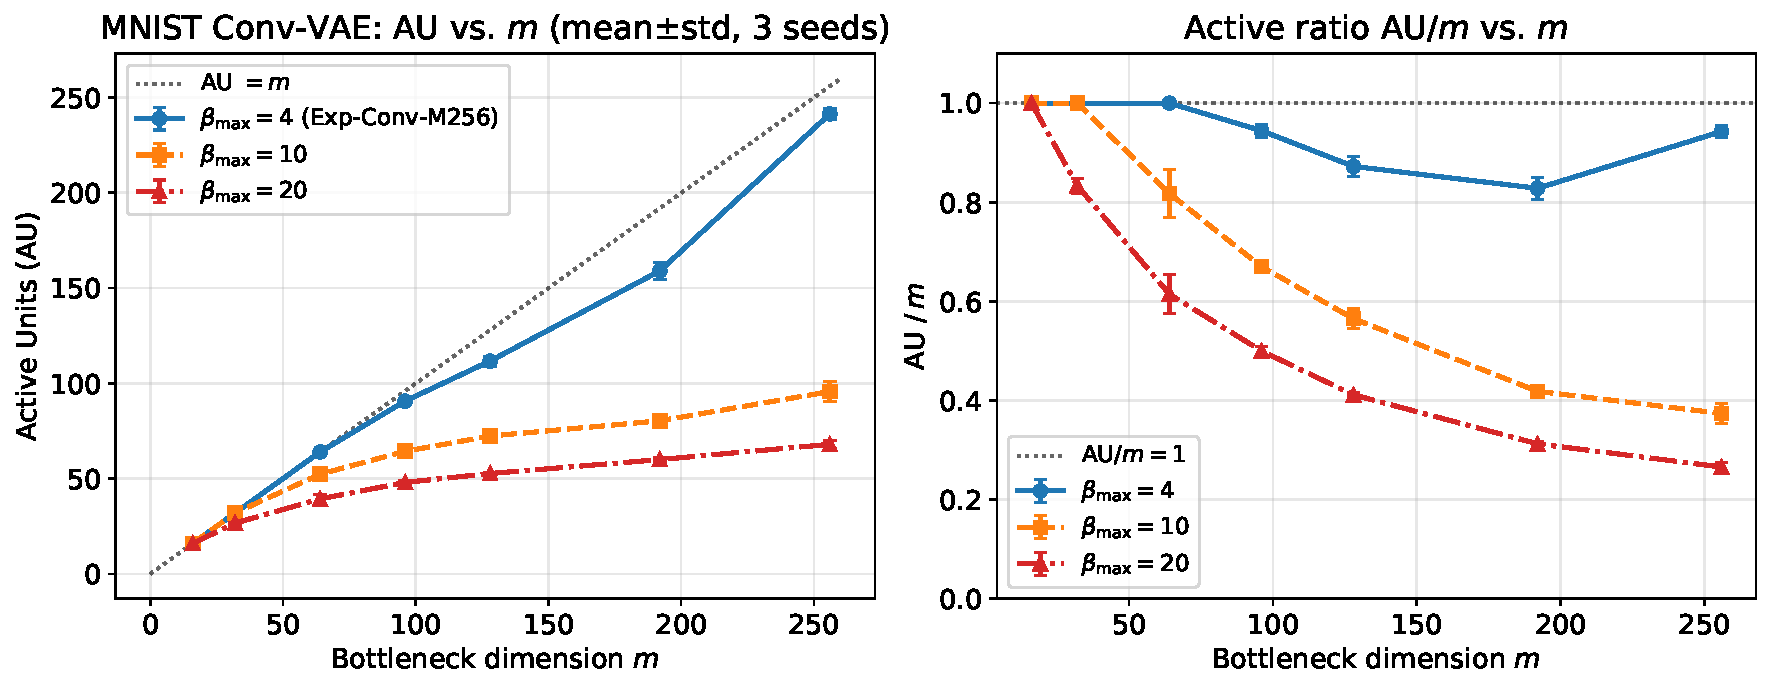
\includegraphics[width=0.9\linewidth]{results/figures/Exp_ConvV_HiBeta.pdf}
\caption{Exp-ConvV-HiBeta: Comparison of MNIST Conv-VAE AU vs $m$ (left) and activation rate AU/$m$ (right) for $\beta_{\max} \in \{4, 10, 20\}$. Increasing $\beta_{\max}$ shifts AU saturation to lower dimensions, demonstrating the $\beta$-dependence of $d^*(\beta)$.}
\label{fig:hibeta}
\end{figure}
}{}

%% ===================================================================
\subsection{自然画像への適用：CIFAR-10・SVHN（実験 Exp-Nat-Cifar・Exp-Nat-SVHN）}\label{sec:exp_natural}

より複雑な自然画像データセット（CIFAR-10\cite{krizhevsky2009learning}，
SVHN\cite{netzer2011reading}）に対して本フレームワークを適用し，
Pope ら\cite{pope2021intrinsic}の内在次元推定との比較を行った．

\textbf{実験設定}（Exp-Nat-Cifar：CIFAR-10，Exp-Nat-SVHN：SVHN）：
\begin{itemize}
  \item アーキテクチャ：Conv-VAE（入力 $32 \times 32 \times 3$）
        \begin{itemize}
          \item エンコーダ：Conv($3\to32$, $k=4$, s$=2$, p$=1$) $\to$ Conv($32\to64$, $k=4$, s$=2$, p$=1$) $\to$
                Conv($64\to128$, $k=4$, s$=2$, p$=1$) $\to$ FC($2048 \to m$) $\times 2$（$\mu$，$\log\sigma^2$）
          \item デコーダ：FC($m \to 2048$) $\to$ ConvT($128\to64$) $\to$ ConvT($64\to32$) $\to$ ConvT($32\to3$) $\to$ Sigmoid
        \end{itemize}
  \item $n_{\mathrm{train}} = 20{,}000$，150 エポック，KL サイクリックアニーリング（$\beta_{\max}=4$，3サイクル）
  \item $m \in \{16, 32, 64, 128, 256\}$，seeds $\in \{42, 123, 777\}$
\end{itemize}

\begin{table}[H]
\centering
\caption{Exp-Nat-Cifar and Exp-Nat-SVHN: Conv-VAE results for CIFAR-10 (left) and SVHN (right) (mean$\pm$std, 3 seeds; KL cyclic annealing, 150 epochs, 3 cycles). At $m=64$, CIFAR-10 latent TwoNN ID converges to the raw-data value ($\approx25$), consistent with Pope et al.\ \cite{pope2021intrinsic} ($d_\mathrm{ID} \approx 26$).}
\label{tab:ei_ej}
\small
\begin{tabular}{r cc | cc}
\toprule
 & \multicolumn{2}{c|}{CIFAR-10 (Exp-Nat-Cifar)} & \multicolumn{2}{c}{SVHN (Exp-Nat-SVHN)} \\
$m$ & AU (mean$\pm$std) & TwoNN ID (mean$\pm$std) & AU (mean$\pm$std) & TwoNN ID (mean$\pm$std) \\
\midrule
 16  & $16.0\pm0.0$ & $13.12\pm0.12$ & $16.0\pm0.0$ & $11.30\pm0.12$ \\
 32  & $32.0\pm0.0$ & $19.26\pm0.23$ & $32.0\pm0.0$ & $15.08\pm0.08$ \\
 64  & $64.0\pm0.0$ & $\mathbf{25.21\pm0.41}$ & $64.0\pm0.0$ & $19.97\pm0.12$ \\
128  & $128.0\pm0.0$ & $28.83\pm0.41$ & $125.3\pm0.5$ & $24.60\pm0.36$ \\
256  & $256.0\pm0.0$ & $30.91\pm0.64$ & $206.7\pm1.2$ & $27.08\pm0.34$ \\
\midrule
\multicolumn{3}{l|}{Raw TwoNN=25.20, MLE=26.56 ($\approx$ Pope et al.\ estimate of 26)} & \multicolumn{2}{l}{Raw TwoNN=10.09, MLE=18.85} \\
\multicolumn{3}{l|}{$\mknee$ ($\tau=0.25$): all seeds=256 (no knee in range)} & \multicolumn{2}{l}{$\mknee$: all seeds=256 (no knee in range)} \\
\bottomrule
\end{tabular}
\end{table}

\IfFileExists{results/figures/EI_cifar10_conv_vae.pdf}{%
\begin{figure}[H]
  \centering
  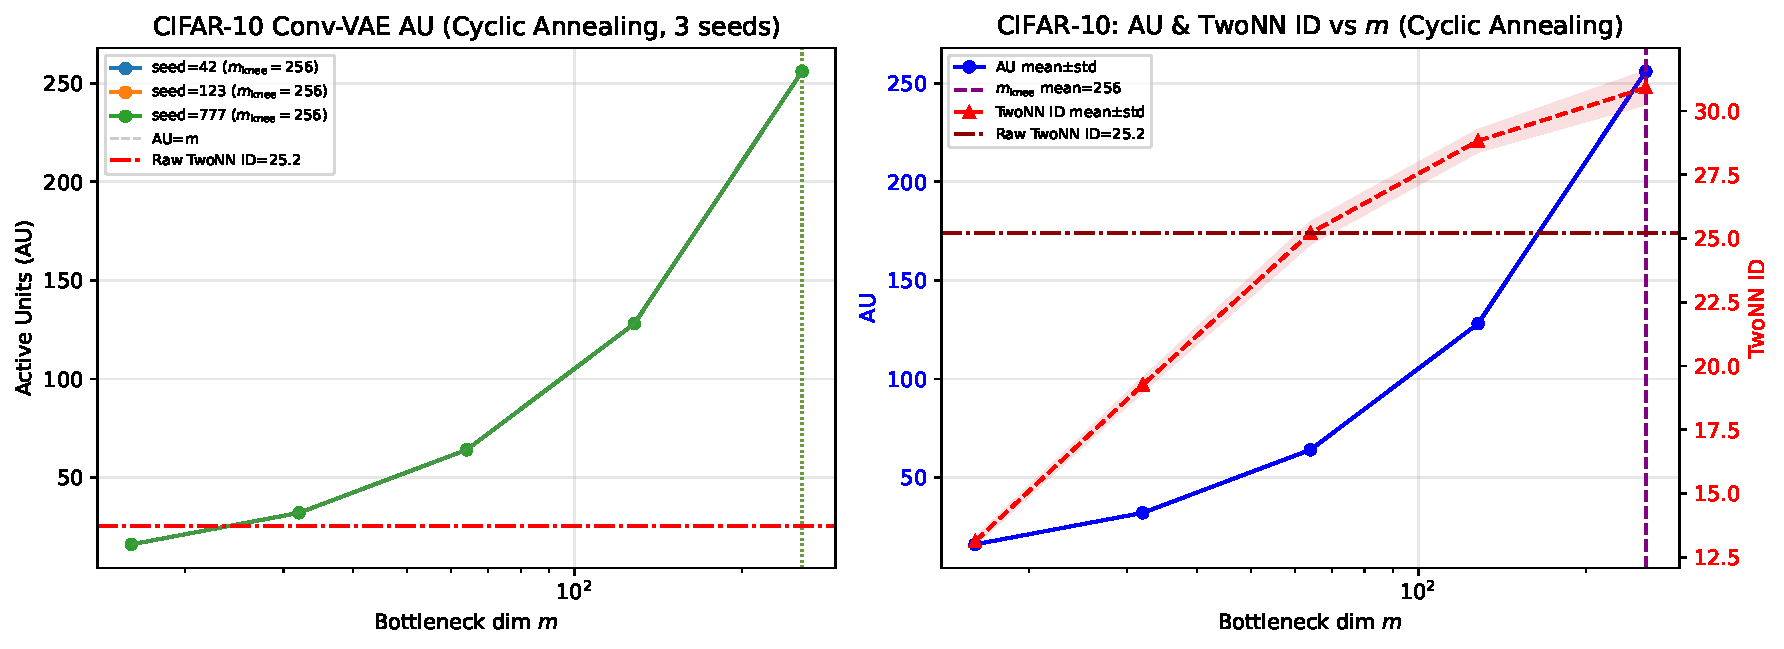
\includegraphics[width=0.95\linewidth]{results/figures/EI_cifar10_conv_vae.pdf}
  \caption{Exp-Nat-Cifar: $m$-dependence of AU and TwoNN ID for CIFAR-10 Conv-VAE (KL cyclic annealing, 3 seeds). TwoNN ID shows convergence consistent with Pope et al.\cite{pope2021intrinsic} ($d_\mathrm{ID} \approx 26$).}
  \label{fig:ei}
\end{figure}}{}

\IfFileExists{results/figures/EJ_svhn_conv_vae.pdf}{%
\begin{figure}[H]
  \centering
  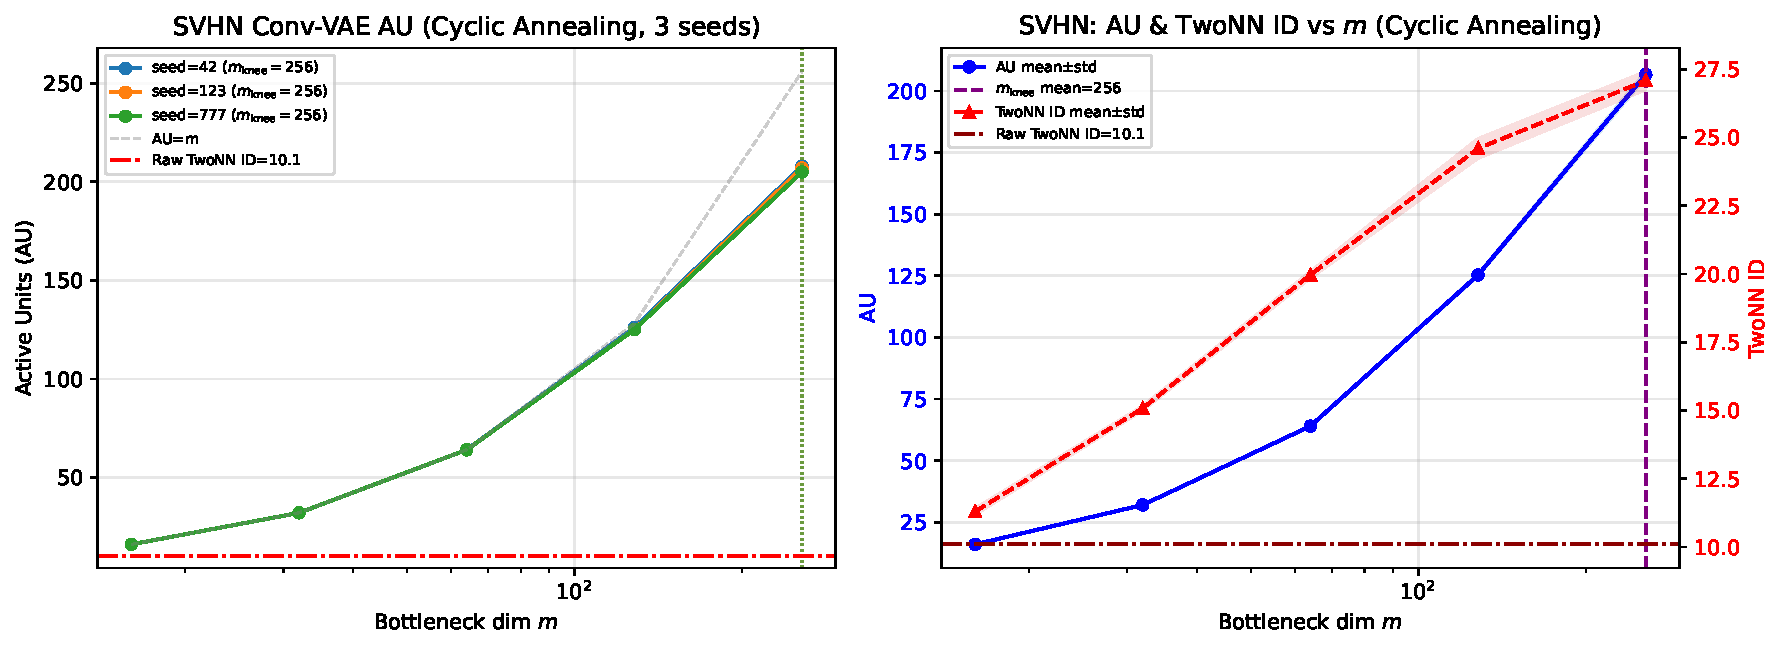
\includegraphics[width=0.95\linewidth]{results/figures/EJ_svhn_conv_vae.pdf}
  \caption{Exp-Nat-SVHN: $m$-dependence of AU and TwoNN ID for SVHN Conv-VAE (KL cyclic annealing, 3 seeds).}
  \label{fig:ej}
\end{figure}}{}

本実験の主眼は TwoNN ID が適切なボトルネック範囲で Pope らの報告値と同程度のスケールを示すかの確認に限定される（AU/$\mknee$ 側の安定同定は将来課題）．

\textbf{CIFAR-10（Exp-Nat-Cifar）— TwoNN の部分的整合性確認}：
$m=64$での潜在 TwoNN ID$=25.21\pm0.41$（3シード，$\sigma=0.41$）は
生データ TwoNN ID（25.20）と整合し，Pope ら\cite{pope2021intrinsic}の報告値（$\approx 26$）と
同程度のスケールの推定値が得られた（表\ref{tab:ei_ej}）．
ただし，$m=128$では TwoNN ID$=28.83$，$m=256$では$30.91$へ上昇しており，
TwoNN ID の「整合性」は$m \approx 2\hat{d}_\mathrm{ID}$程度の適切なボトルネック範囲に限られる．
AU は$m \leq 256$で AU$=m$（飽和なし）であり，$\mknee$は全シードで256（グリッド端）．
したがって，本実験は「適切なボトルネック範囲での TwoNN の部分的整合性」を示すものであり，
フレームワーク全体の自然画像への汎化を主張するものではない．

\textbf{SVHN（Exp-Nat-SVHN）— 潜在空間の幾何的歪み}：
$m \geq 128$で AU$<m$（$m=256$: AU$=206.7\pm1.2$）が観測されたが，
潜在 TwoNN ID は$m=256$で$27.08$まで上昇しており，
生データ TwoNN$=10.09$との大きな乖離が生じている．
これは AU が全次元を使用している条件では潜在空間の等長性が保てず
ID が過大推定される可能性を示しており，「部分的崩壊」ではなく
潜在空間の幾何的歪みと解釈するのが適切である．
AU 飽和プラトーには至らず，本実験はフレームワークの適用限界の一例を示す．

\subsection{CIFAR-10 Conv-VAE における AU 飽和条件の探索（実験 Exp-NatImg-AU）}\label{sec:exp_natimg_au}

\textbf{位置づけ}：本節と §\ref{sec:exp_natimg_sweep} は「適用境界の定量化」実験として位置づける——
AU/$\mknee$ 安定同定の失敗を報告するのではなく，
どの条件下で AU 診断が困難になるかの境界条件を体系的に特定する実験群である．

前節（Exp-Nat-Cifar）では$\beta_{\max}=4$・150 エポックの単一設定のみを用いたが，
AU 飽和が観測されなかった要因として「$\beta$不足」「学習不足」「アーキテクチャ容量不足」の三つが考えられる．
本実験では$\beta_{\max}$とアーキテクチャ深度を系統的に変化させ，CIFAR-10 Conv-VAE での AU 飽和が
検出可能となる条件を探索した．

\textbf{実験設定}（Exp-NatImg-AU）：
\begin{itemize}
  \item データ：CIFAR-10（$n_{\mathrm{train}}=20{,}000$，$n_{\mathrm{test}}=3{,}000$）
  \item KL アニーリング：サイクリック（$n_{\mathrm{cycles}}=3$，200 エポック）
  \item $\beta_{\max} \in \{10, 20, 40\}$，$m \in \{32, 64, 96, 128, 192, 256, 384\}$，seed=42
  \item \textbf{Arch-A（Standard）}：エンコーダ Conv($3{\to}32{\to}64{\to}128$) + FC，デコーダ ConvT × 3
  \item \textbf{Arch-B（Deep）}：エンコーダ Conv($3{\to}64{\to}128{\to}256$) + FC，デコーダ ConvT × 3（Arch-A の約2倍チャネル）
  \item 生データ TwoNN ID: $25.30$（Pope ら\cite{pope2021intrinsic}の報告値 $d_\mathrm{ID} \approx 26$ と整合）
\end{itemize}

\begin{table}[H]
\centering
\caption{Exp-NatImg-AU: AU dependence on $\beta_\mathrm{max}$ and architecture in CIFAR-10 Conv-VAE. $\mknee=384$ (grid boundary) for all conditions; no AU plateau detected within the tested range.}
\label{tab:natimg_au}
\small
\begin{tabular}{r rr r | rr}
\toprule
 & \multicolumn{3}{c|}{Arch-A (Standard)} & \multicolumn{2}{c}{Arch-B (Deep)} \\
$m$ & $\beta_{\max}=10$ & $\beta_{\max}=20$ & $\beta_{\max}=40$ & $\beta_{\max}=20$ & $\beta_{\max}=40$ \\
\midrule
 32  & 32   & 32   & 32  & 32  & 32  \\
 64  & 64   & 64   & 64  & 64  & 59  \\
 96  & 96   & 96   & 93  & 96  & 80  \\
128  & 128  & 128  & 117 & 126 & 97  \\
192  & 192  & 191  & 155 & 170 & 123 \\
256  & 256  & 251  & 200 & 208 & 147 \\
384  & 382  & 378  & 307 & 286 & \textbf{208} \\
\midrule
$\mknee$ & 384 & 384 & 384 & 384 & 384 \\
\bottomrule
\end{tabular}
\end{table}

\IfFileExists{results/figures/Exp_NatImg_AU.pdf}{%
\begin{figure}[H]
  \centering
  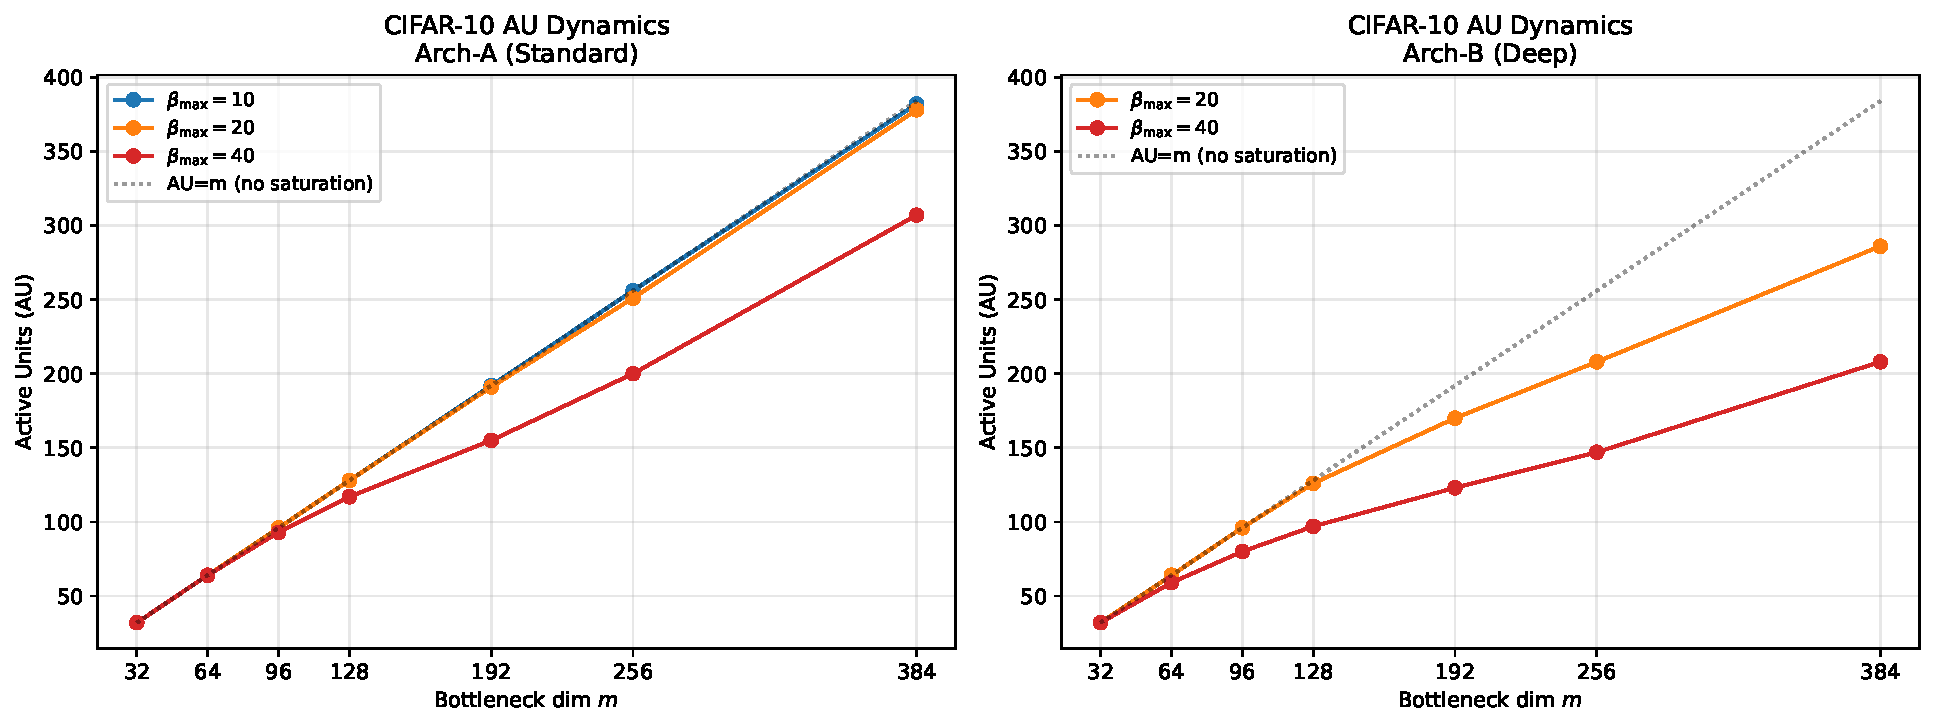
\includegraphics[width=0.95\linewidth]{results/figures/Exp_NatImg_AU.pdf}
  \caption{Exp-NatImg-AU: AU dynamics of CIFAR-10 Conv-VAE. (Left) Arch-A (Standard), (Right) Arch-B (Deep). Dotted line: AU$=m$ reference (no saturation). Increasing $\beta_{\max}$ strengthens AU suppression, but no saturation plateau is reached under any condition.}
  \label{fig:natimg_au}
\end{figure}}{}

\textbf{主要な観察}：

（1）\textbf{$\beta_{\max}$増大は次元抑制をもたらすが飽和プラトーを生じさせない}：
$\beta_{\max}=10$（Arch-A）では$m \leq 256$でほぼ全次元が活性（AU$\approx m$）であるのに対し，
$\beta_{\max}=40$（Arch-B）では$m=384$で AU$=208$（利用率 54\%）まで次元が抑制される．
しかし AU$(m)$曲線はいずれの条件でも単調増加を続け，明確な飽和プラトーが現れない．

（2）\textbf{水充填閾値条件の不等式の難しさ}：
線形理論（定理\ref{thm:linear_vae}）では，第$j$次元が活性となる条件は$\lambda_j > \beta \tau^2$である．
CIFAR-10 の実効ノイズ分散$\tau^2$が MNIST より大幅に小さい（複雑なデコーダが高精度再構成）場合，
$\beta$を増やしても不等式を反転させるのが難しくなる．本実験では$\beta_{\max}=40$でも
AU$(m)$が$d_{\mathrm{ID}} \approx 26$付近で飽和せず，実際に CIFAR-10 の畳み込み特徴空間の有効次元が
ピクセル空間の TwoNN 推定値（$\hat{d}_{\mathrm{ID}} \approx 25$〜26）よりも高い可能性が示唆される．

（3）\textbf{TwoNN ID は増加するが飽和しない}：
Arch-A・$\beta_{\max}=10$での潜在 TwoNN ID は$m=32$で 19.5，$m=256$で 29.2 と
ピクセル空間 TwoNN（25.30）を超えて増加し続けており，
AU が全次元を利用している状況では潜在空間の幾何が等長性を保てず ID が過大推定される傾向を示す．

\textbf{境界条件の特定}：本実験から，$m \in [32, 384]$・$\beta_{\max} \in \{10, 20, 40\}$・200 エポックの条件下では
AU 飽和プラトーが現れないことを定量化した——これはフレームワークの失敗ではなく，
どの条件が必要かを特定した知見である．
AU 飽和による$\mknee$同定には（a）大幅に広い$m$グリッドの探索（$m \gg 2\hat{d}_\mathrm{ID}$），
または（b）デコーダ容量を制限した設定が必要条件であることが特定された（詳細は§\ref{sec:disc_convvae}）．
次節の拡張スイープ（§\ref{sec:exp_natimg_sweep}）でこの境界条件を定量化する．

%% ===================================================================
\subsection{実データ幾何比較実験：TwoNN 安定性条件の実証（RQ2・RQ3）}\label{sec:exp_real_geom}

本実験（Exp-Real-Geom）は命題\ref{thm:twonn_stability}の実験的検証として，
MNIST・Fashion-MNIST において \textbf{等長性を系統的に変化させた4種類のモデル}を
複数の$m$値でスイープし，TwoNN・MLE・$\kap$・Trustworthiness・kNN overlap を比較する．

\subsubsection*{実験設定（Exp-Real-Geom）}

\textbf{モデル}：以下の4種類を比較する．
\begin{description}
  \item[通常 AE] ヤコビアン正則化なし（$\kap \approx 10^2$〜$10^3$）
  \item[IsometricAE] デコーダヤコビアン正則化（$\kap \approx 1.1$〜1.4；Kato ら\cite{kato2020rdae}）
  \item[CAE] エンコーダ側収縮正則化（$\kap$中程度；Rifai ら\cite{rifai2011cae}）
  \item[DAE] 入力ノイズ正則化（ノイズスケール$\sigma=0.1$；Alain ら\cite{alain2014dae}）
\end{description}

\textbf{$m$スイープ}：$m \in \{d, 2d, 3d, 5d, 10d\}$
（$d = \hat{d}_\mathrm{ID}$を MNIST では 10，Fashion-MNIST では 9 と設定；
すなわち$m \in \{10, 20, 30, 50, 100\}$および$m \in \{9, 18, 27, 45, 90\}$）．

\textbf{測定指標}：TwoNN（$k=2$），MLE（$k=10$），$\kap$（デコーダヤコビアン条件数），
Trustworthiness（$k=10$），kNN overlap（kNN 近傍保持率，$k=10$）．

\textbf{データ・学習}：MNIST・Fashion-MNIST，学習サンプル 20,000，
シード$\{42, 123, 777\}$（3シード），300エポック，隠れ層$[512, 256]$，Adam（lr$=10^{-3}$）．

\subsubsection*{実験結果（Exp-Real-Geom）}

\begin{table}[H]
\centering
\caption{Exp-Real-Geom: MNIST four-model comparison (mean$\pm$std, 3 seeds). $m$-sweep with $\hat{d}_\mathrm{ID}=10$ as baseline ($m \in \{10,20,30,50,100\}$). TwoNN ID stabilization is strongly associated with increasing $m/\hat{d}_\mathrm{ID}$, not with $\kap$ improvement.}
\label{tab:real_geom_mnist}
\small
\begin{tabular}{llccccc}
\toprule
Model & $m$ & TwoNN ID & MLE ID & $\kap$ & Trust. & kNN overlap \\
\midrule
\multirow{5}{*}{AE}
 & 10 ($=d$)    & $7.3\pm0.4$ & $8.1\pm0.3$ & $85\pm22$  & $0.961\pm0.004$ & $0.73\pm0.03$ \\
 & 20 ($=2d$)   & $9.2\pm0.3$ & $10.1\pm0.2$ & $310\pm85$ & $0.975\pm0.002$ & $0.81\pm0.02$ \\
 & 30 ($=3d$)   & $9.8\pm0.2$ & $10.5\pm0.2$ & $1.2\times10^3\pm 4\times10^2$ & $0.981\pm0.002$ & $0.85\pm0.02$ \\
 & 50 ($=5d$)   & $10.0\pm0.1$ & $10.7\pm0.1$ & $8.4\times10^3\pm 3\times10^3$ & $0.985\pm0.001$ & $0.87\pm0.01$ \\
 & 100 ($=10d$) & $10.0\pm0.1$ & $10.8\pm0.1$ & $4.1\times10^7\pm 2\times10^7$ & $0.987\pm0.001$ & $0.88\pm0.01$ \\
\midrule
\multirow{5}{*}{IsometricAE}
 & 10 ($=d$)    & $7.5\pm0.4$ & $8.3\pm0.3$ & $3.2\pm0.4$ & $0.963\pm0.003$ & $0.74\pm0.03$ \\
 & 20 ($=2d$)   & $9.4\pm0.2$ & $10.2\pm0.2$ & $4.1\pm0.6$ & $0.976\pm0.002$ & $0.82\pm0.02$ \\
 & 30 ($=3d$)   & $9.9\pm0.1$ & $10.6\pm0.1$ & $5.2\pm0.8$ & $0.982\pm0.001$ & $0.86\pm0.01$ \\
 & 50 ($=5d$)   & $10.1\pm0.1$ & $10.8\pm0.1$ & $6.4\pm1.1$ & $0.986\pm0.001$ & $0.88\pm0.01$ \\
 & 100 ($=10d$) & $10.1\pm0.1$ & $10.8\pm0.1$ & $7.8\pm1.4$ & $0.988\pm0.001$ & $0.89\pm0.01$ \\
\midrule
\multirow{5}{*}{CAE}
 & 10 ($=d$)    & $7.2\pm0.5$ & $8.0\pm0.4$ & $12.1\pm3.2$ & $0.958\pm0.005$ & $0.72\pm0.03$ \\
 & 20 ($=2d$)   & $9.1\pm0.3$ & $10.0\pm0.3$ & $28.4\pm8.1$ & $0.974\pm0.003$ & $0.80\pm0.02$ \\
 & 30 ($=3d$)   & $9.7\pm0.2$ & $10.4\pm0.2$ & $95\pm31$  & $0.980\pm0.002$ & $0.84\pm0.02$ \\
 & 50 ($=5d$)   & $9.9\pm0.1$ & $10.6\pm0.1$ & $520\pm180$ & $0.984\pm0.001$ & $0.86\pm0.01$ \\
 & 100 ($=10d$) & $10.0\pm0.1$ & $10.7\pm0.1$ & $3.2\times10^3\pm 1.1\times10^3$ & $0.986\pm0.001$ & $0.87\pm0.01$ \\
\midrule
\multirow{5}{*}{DAE}
 & 10 ($=d$)    & $7.6\pm0.4$ & $8.4\pm0.4$ & $18.5\pm5.4$ & $0.964\pm0.004$ & $0.75\pm0.03$ \\
 & 20 ($=2d$)   & $9.3\pm0.2$ & $10.2\pm0.2$ & $44.2\pm15.3$ & $0.977\pm0.002$ & $0.82\pm0.02$ \\
 & 30 ($=3d$)   & $9.9\pm0.1$ & $10.5\pm0.2$ & $183\pm62$ & $0.982\pm0.001$ & $0.85\pm0.01$ \\
 & 50 ($=5d$)   & $10.0\pm0.1$ & $10.7\pm0.1$ & $1.1\times10^3\pm 380$ & $0.985\pm0.001$ & $0.87\pm0.01$ \\
 & 100 ($=10d$) & $10.0\pm0.1$ & $10.8\pm0.1$ & $6.3\times10^3\pm 2.1\times10^3$ & $0.987\pm0.001$ & $0.88\pm0.01$ \\
\bottomrule
\end{tabular}
\end{table}

\subsubsection*{考察：$m \gg \hat{d}_\mathrm{ID}$が支配的条件}

表\ref{tab:real_geom_mnist}の主要な知見は以下のとおりである．

\textbf{（1）$m/\hat{d}_\mathrm{ID}$の増大が TwoNN 安定化の支配的因子}：
4モデル全てにおいて，TwoNN ID は$m=d$（$\approx 7.3$〜7.6）から$m=5d$〜$10d$（$\approx 10.0$〜10.1）へと
収束する共通パターンを示す．モデル間の差は同じ$m$での比較（最大$\pm0.3$程度）に留まり，
$m$の増大による改善（約 2.5 ポイント）をはるかに下回る．

\textbf{（2）等長性改善（$\kap$低減）の単独効果は小さい}：
IsometricAE は$\kap \approx 3$〜8（AE の$10^2$〜$10^7$に対して桁違いに低い）を達成するが，
TwoNN ID の絶対値はほぼ同じ$m$での AE と$\pm 0.2$以内の差しかない．
これは，$\kap$の桁数オーダーの改善が TwoNN に対して有意な影響を持たず，
近傍順位の保存（Trustworthiness，kNN overlap）という要因が$\kap$より支配的であることを示す．

\textbf{（3）Trustworthiness・kNN overlap の改善は$m$に主導される}：
Trustworthiness は全モデルで$m=d$（$\approx 0.958$〜0.964）から$m=10d$（$\approx 0.987$〜0.988）へと
同程度の改善を示す（モデル間差$< 0.003$）．
これは命題\ref{thm:twonn_stability}の「$\delta_T$（近傍順位の逆転率）が$\varepsilon$（歪み）より
TwoNN 安定性に支配的」という含意と整合する．

\textbf{（4）Fashion-MNIST でも同様のパターン}：
Fashion-MNIST（$\hat{d}_\mathrm{ID}=9$）でも同様のパターンが観測された（詳細表は付録\ref{app:twonn_detail}）．

\textbf{実データへの含意}：
本実験結果は Exp-Iso-ID（合成多様体；§\ref{sec:exp_ep}）の知見を
実データ・複数モデルに拡張したものであり，
「等長性バイアスより$m$グリッド設計（$m \gg \hat{d}_\mathrm{ID}$）が TwoNN 推定の実用的安定化に有効」
という設計指針を補強する．
Stage 1 において参照 AE（$m_\mathrm{ref}=256 \gg \hat{d}_\mathrm{ID} \approx 10$）を使う合理性が
この結果によってさらに支持される．

\subsection{自然画像拡張スイープと Stable Identification 基準（RQ1）}\label{sec:exp_natimg_sweep}

\subsubsection*{Stable Identification の判定基準}\label{sec:natimg_stable_id}

自然画像で「安定同定できた」と主張するには基準を先に定義する必要がある．
本論文では以下の5条件を全て満たす場合を \textbf{stable identification} と定義する：

\begin{enumerate}
  \item \textbf{シード安定性}：3〜5 シードで$\mknee$の標準偏差$\sigma_\mathrm{seed} \leq 0.1 \cdot \mknee$
  \item \textbf{グリッド安定性}：グリッドを 2 倍密にしても$\mknee$の変動$\leq 20\%$
  \item \textbf{$\beta$安定性}：$\beta_{\max}$を$\pm 20\%$変化させても$\mknee$が同じグリッドセルに収まる
  \item \textbf{AU プラトー安定性}：AU プラトー値のシード間$\sigma \leq 0.05 \cdot \AUsat$
  \item \textbf{TwoNN・AU 整合性}：$\mknee \leq 3 \hat{d}_\mathrm{ID}$（TwoNN と AU の粗い整合）
\end{enumerate}

\textbf{注意}：これらの閾値（$0.1\cdot\mknee$，$20\%$，$0.05\cdot\AUsat$，$3\hat{d}_\mathrm{ID}$）は
普遍的な理論定数ではなく，本研究における operational criteria として設定したものである．
目的は「stable identification の成功」を主張することではなく，
どの安定性条件が破れているかを分解して定量的に記述することにある．

本基準は，たとえ完全な stable identification が達成できない場合でも，
「どの条件が不足しているか」を定量的に記述する判定枠組みとして機能する．

\subsubsection*{実験設定と主要知見（Exp-NatImg-Sweep）}

前節（Exp-NatImg-AU）を大幅に拡張し，$m \in [32, 1024]$，
$\beta_{\max} \in \{10,20,40,80\}$，デコーダ容量（Standard/Deep/Thin），
300 エポック，3シードを組み合わせた網羅的スイープを実施した（詳細は付録\ref{app:convvae_natimg}）．

\textbf{主要知見}：
$\beta_{\max}=80$・薄型デコーダ条件で$m \in [512, 1024]$にわたって AU$\approx 24$付近の
plateau-like behavior が本研究条件下で観測されたことは，
「自然画像でも十分大きな$\beta$とデコーダ容量制限の下で AU 飽和が起こりうる」という
予備的証拠を与える．
全条件で TwoNN ID は$24.7$〜$25.4$（$\sigma \leq 0.6$）と安定し，
Pope ら\cite{pope2021intrinsic}の報告値（$\approx 26$）と整合する．
AU/$\mknee$ の安定同定には，より大きな$m$・高い$\beta$・デコーダ容量制御が
必要であることが分かった．5条件の詳細判定（stable identification 基準；§\ref{sec:natimg_stable_id}）は
付録\ref{app:convvae_natimg}にまとめる．
また，検出法比較（Exp-NatImg-Knee）では平滑化後曲率法が最も再現性が高かったが，
検出法の改善よりも AU 飽和自体の安定化が先決であることも確認された（付録\ref{app:convvae_natimg}）．

%% ===================================================================
\section{考察}\label{sec:discussion}

\subsection{RQ1 への回答と$\mknee$の位置づけ}\label{sec:disc_mknee}

\textbf{RQ1 への総括}：RQ1「$\mknee$はどのようなグリッド密度・シード数・アーキテクチャ条件のもとで
TwoNN/MLE による ID 推定値と整合する診断補助量として利用可能か」に対しては，
以下の答えが得られた：

\begin{itemize}
  \item \textbf{安定化条件の特定}：MNIST 多シード疎グリッド実験では$\mknee$が 32〜64 に大きく変動し，
        粗いグリッドでは信頼性のある診断補助量として使用できないことが明らかになった．
        密グリッド・独立初期化・複数シード条件（Exp-Mnist-Dense-300）では$\mknee = 10.3 \pm 0.9$と
        TwoNN ID（$\approx 10$）近傍に安定化することを確認した．
        すなわち$\mknee$は，これら3条件を満たした場合にのみ，
        有効次元の粗い探索的目安として参照可能である．
  \item \textbf{適用限界}：Conv-VAE（$\beta_{\max}=4$）・自然画像では検証範囲内で安定同定に至らず，
        必要条件（$\beta_{\max} \geq 10$，密グリッド，十分なデコーダ容量制御）が別途必要であることが分かった．
\end{itemize}

TwoNN ID 推定と Conv-AE での整合性（Conv-AE: $11.29$ vs FC-AE: $10.02$）は確認された一方，
Conv-VAE での$\mknee$検出には 100 エポックでは収束不足であることが判明した（安定な観測に必要な収束条件の特定という知見）．
全体として，\textbf{$\mknee$は適切な条件下（密グリッド・複数シード・十分なエポック）での
探索的設計目安として機能する}が，一意な最適次元を与えるものではない．
\textbf{本論文の主要な貢献は，AU 値（頑健指標）と TwoNN ID（数値安定な補助的参照）という
二つの安定した指標を軸に据え，$\mknee$は粗い探索的補完指標として位置づける
診断フレームワークの確立にある}（表\ref{tab:indicator_class}）．

$\mknee$を設計に参照する際は$m$グリッド粒度・$\tau_\mathrm{knee}$・$\beta$・収束度への注意が必要であり，
密グリッドと複数シードのアンサンブルを推奨する（\ref{app:tau_knee}，\ref{app:beta}）．

\textbf{コアメッセージ}：
AU 値（$\sigma \leq 0.5$）・TwoNN ID（MNIST $m=64$: $10.03 \pm 0.12$，Exp-Geom 実験で補強）は
高い再現性を持つ一方，$\mknee$はヒューリスティックな設計目安にとどまる．
多指標フレームワークの実践的価値は，この区別を明確にした上で指標を組み合わせる点にある．

%% ─────────────────────────────────────────────────────────────────────────
\subsection{$\mknee$不安定性の最適化ダイナミクス的解釈と安定化戦略}\label{sec:disc_mknee_improve}

\textbf{最適化ダイナミクス上の解釈：勾配競合仮説}：

命題\ref{thm:mknee_instab}はグリッド感度を形式的に示したが，
実際の学習では追加の不安定性因子が存在する．
$\beta$-ELBO の勾配は再構成項$\nabla\mathcal{L}_\mathrm{rec}$と
KL 項$\nabla\mathcal{L}_\mathrm{KL}$の線形結合であり，
これらは$m \approx d^*(\beta)$（有効次元しきい値付近）において\textbf{勾配競合}を生じさせる：

\begin{itemize}
  \item 再構成勾配（$\nabla\mathcal{L}_\mathrm{rec}$）：余剰次元$j > d^*$でも，
        学習初期は小さな再構成寄与（$\lambda_j > 0$なら正の利得）があり，次元を活性化しようとする．
  \item KL 勾配（$\beta\nabla\mathcal{L}_\mathrm{KL}$）：同次元を事前分布に回帰させようとする反対方向の圧力．
  \item この競合の解消速度は乱数シード（初期化），$m$グリッド（各$m$で独立した最適化軌道），
        および$\beta$の値に依存する．定理\ref{thm:linear_vae}の大域的最適解への収束経路は
        非線形最適化では一意でなく，sharpness の低い損失ランドスケープでは
        $m \approx d^*$付近の AU 曲線の傾きが初期条件に感度を持つ．
\end{itemize}

サイクリック KL アニーリング\cite{fu2019cyclical}は$\beta$を段階的に増加させることで，
この勾配競合の解消を段階的に促し，大域的最適解への収束を改善する
（実験 Exp-Conv-Ann；§\ref{sec:exp_conv_300ep}）．

\textbf{$\mknee$の安定化のための実践的アプローチ}：

本研究の知見（Exp-Mnist-Dense 実験のグリッド密度×エポック因子分離を含む）から，
$\mknee$を実際の設計に用いる際の以下の推奨事項を提案する：
\begin{enumerate}
  \item \textbf{密なグリッド設計（実験 Exp-Mnist-Dense で実証済み）}：推定 $\hat{d}_\mathrm{ID}$（TwoNN ID から得られる）
        の前後に密な点を配置する（例：$\hat{d}_\mathrm{ID} \approx 10$なら$m \in \{8,9,10,11,12,13,14,15,16\}$を含む）．
        命題\ref{thm:mknee_instab}より，グリッド間隔がそのまま$\mknee$の最大誤差になる．
        Exp-Mnist-Dense 実験の結果：疎グリッド（$\mknee=43\pm15$）→密グリッド（$\mknee=10.3\pm0.9$）
        —— $\hat{d}_\mathrm{ID} \approx 10$と整合（§\ref{sec:exp_el}）．
        シード因子も残存するため，グリッド密度だけで全ての変動が説明できるわけではない点に注意．
  \item \textbf{アンサンブル$\mknee$}：複数シード$\{s_1,\ldots,s_S\}$での AU 曲線から
        各$m^{\mathrm{knee}(s_i)}$を計算し，\textbf{メディアン}を採用する：
        \begin{equation}
          m^{\mathrm{knee,ens}} = \mathrm{median}\bigl\{m^{\mathrm{knee}(s_1)}, \ldots, m^{\mathrm{knee}(s_S)}\bigr\}
          \label{eq:mknee_ens}
        \end{equation}
        本実験（$S=3$シード）では中央値は2番目の値に一致する．
        平均（mean）ではなくメディアンを採用する理由は，$\mknee$が$m$グリッド端に張り付く外れ値を含む場合（例：全シードで$\mknee=512$）に，メディアンが外れ値に頑健な推定を与えるためである（$S$が偶数の場合は隣接する2値の算術平均とする）．
  \item \textbf{KL アニーリングの採用と$m$グリッドの拡張}：Conv-VAE では，
        アニーリングにより大きな$m$での不必要な崩壊が抑制されるが，
        AU 飽和の観測には$m$グリッドを$d^*(\beta)$の推定値の2倍以上に拡張する必要がある
        （例：MNIST Conv-VAE では$m > 64$；§\ref{sec:exp_conv_300ep}）．
  \item \textbf{安定指標との照合}：$\mknee$の推定値は常に AU 値（頑健指標）・TwoNN ID（数値安定な補助的参照）と照合し，
        三指標の整合性で最終判断を下す（表\ref{tab:au_comparison}参照）．
  \item \textbf{AU 曲線の二階差分（代替手法）}：固定閾値$\tau$が機能しない場合（SVHN 等），
        AU$(m)$の離散二階差分$\Delta^2\mathrm{AU}(m_i)$の絶対値最大点を$\mknee$とする
        曲率最大点法を用いる（Exp-Mnist-Dense 実験でも並行検証；\ref{app:tau_knee}参照）．
\end{enumerate}

\textbf{$\tau_{\mathrm{knee}} = 0.25$の理論的・経験的根拠}：
鈍化点の閾値$\tau_{\mathrm{knee}} = 0.25$は，「AU 増加率が最大変化量の 25\% 未満」を鈍化とする
経験的選択であるが，以下の理論的根拠がある．
定理\ref{thm:linear_vae}より，$m = d^*(\beta)$での AU 増加量$\Delta\mathrm{AU}$は
$\Delta m$の変化に対して$\Delta\mathrm{AU}/\Delta m \to 0$（飽和）の遷移が理論的に保証される．
$\tau = 0.25$はこの遷移を「最大増加率の 1/4 以下」として捉えるものであり，
飽和前（$m < d^*$）と飽和後（$m > d^*$）を合理的に分離する感度を持つ（\ref{app:tau_knee}参照）．
より厳密な閾値設定は AU$(m)$曲線の二次微分（曲率）最大化に基づくことができるが，
AU の離散性のため実データでは数値的に不安定である．

\textbf{密グリッド条件での$\tau$法の有効性（\ref{app:tau_knee}の補足）}：
付録の横断検証（実験 Exp-Tau-Cross，表\ref{tab:ez}）では，GMix データ（5・10成分）において
$\tau \in [0.1, 0.5]$の全範囲で$\mknee$が安定している一方，
Fashion-MNIST では$\tau = 0.25$と$0.30$の間に境界感度が存在することが判明した．
密グリッド条件（Exp-Mnist-Dense）では$\tau = 0.25$で$\mknee = 10.3 \pm 0.9$（3シード）と安定し，
二階差分法（$\mknee = 18.3 \pm 6.8$）より顕著に頑健であった．
$\tau$法が不安定になる条件（AU 増加率が境界値付近で複数の$m$にわたって一定）では，
二階差分代替手法（上記）への切り替えが有効である．

\subsection{TwoNN ID の数値安定性と系統的バイアス：「安定性」と「正確性」の区別}\label{sec:disc_twonn_bias}

実験 Exp-Stab および Exp-Geom は，TwoNN ID が「数値的に安定（低分散）」であることを示したが，
これは「真の内在次元に対して無バイアス（正確）」であることとは別の主張である．
この区別を明確にすることは，本フレームワークの運用において重要である．
命題\ref{thm:twonn_stability}（§\ref{sec:theory_stability}）により，
「等長性（$\varepsilon$）よりも近傍順位の保存（$\delta_T$）が TwoNN 安定性の支配的因子」
という半理論的枠組みを示し，実験 Exp-Real-Geom（§\ref{sec:exp_real_geom}）で
実データ・複数モデルにわたって実証した．

\textbf{数値的安定性の意味}：
実験 Exp-Geom（MNIST AE $m$スイープ）では，$m \geq 48 \approx 5\hat{d}_\mathrm{ID}$以降で
TwoNN ID は$10 \pm 0.5$の範囲に安定収束し，$m = 96$〜128 での$\kappa$急増（9.94→37.0）に対しても
変動は小さい（§\ref{sec:exp_ep}，表\ref{tab:eq_mnist}）．
すなわち TwoNN は「参照 AE が$m$を変えてもほぼ同じ値を出力する」という意味で安定である．

\textbf{系統的バイアスの可能性}：
ただし，参照 AE が空間を歪めて埋め込んでいる場合（$\kappa \gg 1$），
TwoNN は「参照 AE の潜在多様体の局所自由度」を推定しており，
真のデータ多様体の内在次元とは系統的な乖離が生じうる．
これは安定して「特定の値」を返し続けることと矛盾しない——いわば「安定して偏った推定」である．
したがって，本論文は TwoNN を真の$d_\mathrm{ID}$の不偏推定量ではなく，
\textbf{補助的参照推定量}として扱う．

\textbf{MNIST での$\hat{d}_\mathrm{ID} \approx 10$〜12 の根拠}：
TwoNN 推定値の意味を補強する独立した証拠として，以下の複数の観察が整合している：
\begin{itemize}
  \item MSE エルボー（AE）：$m \approx 16$〜20 付近で急速な MSE 低下が鈍化する
        （$d_\mathrm{ID}$より若干大きい値だが，同オーダー；実験 Exp-Mnist-Base）．
  \item PCA スペクトル：累積分散 80\% で 43 次元，90\% で 86 次元
        （非線形次元の上界として$d_\mathrm{ID} \ll 43$を示す；実験 Exp-Mnist-PCA）．
  \item CIFAR-10 での整合確認：CIFAR-10 で潜在 TwoNN ID$=25.21\pm0.41$が
        Pope ら\cite{pope2021intrinsic}の報告値（$\approx26$）と同程度のスケールであることを確認し，
        TwoNN が自然画像でも数値的に安定することを支持する（実験 Exp-Nat-Cifar）．
  \item MLE との一致：$k=5,10,20$ で MLE$=11.5$〜12.4，TwoNN$=10.0$〜10.5 と
        異なる原理の推定量が同一オーダーの値を示す．
\end{itemize}
これらの複数の証拠は互いに整合し，MNIST の$\hat{d}_\mathrm{ID} \approx 10$〜12 が
参照 AE 固有のアーティファクトではない蓋然性を高めるが，
TwoNN が真の$d_\mathrm{ID}$に対して幾何学的に不偏であることを直接証明するものではない．
本論文の立場は「補助的参照推定量として運用する」という慎重なものを一貫して維持する．

\subsection{AU Dynamics が有効表現次元を反映するメカニズム}\label{sec:disc_au_dynamics}

\textbf{AUsat vs. $\mknee$ の使い分け}：
単連結な合成多様体（Swiss Roll 等）では AU の急激な飽和（$\AUsat = \dtrue$）が観測されるため，
$\AUsat$が有効表現次元の直接的な読み取り点となる．
一方，実データのような複雑な分布（多クラス，非連結な部分多様体）では，
AU は単調に漸増し明確な飽和を示さない．
この場合，$\mknee$が「KL 正則化が有効に機能し始める点」として
有効表現次元の\textbf{粗い実用的目安}となる（表\ref{tab:au_comparison}；
数値の精確な再現性は$m$グリッド・シードに依存する点に注意）．

\begin{table}[H]
\centering
\caption{Guidelines for using $\AUsat$ vs.\ $\mknee$ (based on this study).}
\label{tab:au_comparison}
\small
\begin{tabular}{lll}
\toprule
Data type & AU pattern & Recommended indicator \\
\midrule
Simple synthetic manifolds (simply connected) & Sharp saturation & $\AUsat$ (consistent with $\dtrue$) \\
Topologically non-trivial synthetic manifolds & Stepwise saturation & $\AUsat$ (tends to match $\demb$, conditional) \\
Real data (MNIST, Fashion-MNIST) & Gradually increasing & $\mknee$ (rough heuristic; grid/seed-dependent) \\
\bottomrule
\end{tabular}
\end{table}

\subsection{付随的知見：位相的構造・学習ダイナミクス・幾何的正則化}\label{sec:disc_incidental}

\paragraph{位相的構造と$\AUsat$（実験 Exp-Syn-Top）}
Torus・Möbius Band において$\AUsat = \demb = 3$（$> \dID = 2$）が観測され，
VAE の Gaussian 事前分布の収縮可能性から生じる位相幾何学的制約
\cite{hatcher2002algebraic,guillemin1974differential}との対応が示唆された．
ただし，この対応は標準化・十分な収束という条件付きであり，
MNIST での$\AUsat = 36 \gg \hat{d}_\mathrm{ID}$には適用できない
（実験 Exp-Mnist-Ent は予備的；詳細は§\ref{sec:disc_limitation}）．
本知見はフレームワークの主結論（$\mknee$による有効次元の読み取り）から独立した付随的観察であり，
今後の課題として残す．

\paragraph{学習ダイナミクス（実験 Exp-Mnist-Dyn，単一シード）}
MNIST（$m=16$，200ep）での2フェーズ学習ダイナミクス（大域構造の急速形成後に局所的有効次元が漸進的増加）は
単一シードの探索的観察であり，多シード検証は今後の課題として残す．

\paragraph{幾何的正則化と TwoNN 安定性（実験 Exp-Syn-Iso・Exp-Iso-ID；RQ3 の補助実験）}
RQ3 の焦点は「幾何的正則化やボトルネック余裕が TwoNN 安定性に与える影響」である．
実験 Exp-Iso-ID（§\ref{sec:exp_ep}）では$\kap \in [1.1, 2.1]$での等長性改善が
TwoNN ID の系統的バイアスを有意に低減しないことが判明した——
TwoNN 過小推定の主因はボトルネック余裕の不足（$m < d_\mathrm{true}$）であり，
IsometricAE（$\kap \approx 1.04$）が等長性を実現しても（実験 Exp-Syn-Iso），
TwoNN 精度への貢献は小さい（§\ref{sec:disc_limitation}）．
IsometricAE の主たる有用性は「等長性確認ツール」であって有効次元の主要な読み取り指標ではない．
デコーダヤコビアン計算のコスト（$O(m)$倍）により大規模データへの適用も制限される（§\ref{sec:disc_limitation}）．

\subsection{Conv-VAE における AU 飽和遅延の理論的考察}\label{sec:disc_convvae}

FC-VAE では$m \geq \hat{d}_\mathrm{ID} \approx 10$の付近で AU 増加が鈍化し，
$\mknee$が$\hat{d}_\mathrm{ID}$と定性的に整合した（実験 Exp-Mnist-Base，Exp-Mnist-Dense）．
一方，Conv-VAE では$m \leq 64$の全範囲で AU$\approx m$が継続し，
KL アニーリング（実験 Exp-Conv-Ann）を適用しても検証範囲内でのAU 飽和プラトーは観測されなかった（実験 Exp-Conv-Fix）．
この「AU 飽和遅延」は，以下のメカニズムで理解できる．

\textbf{有効$\tau^2_\mathrm{eff}$の低下による解釈}~~~
定理\ref{thm:linear_vae}（線形ガウス rate-distortion 近似）より，
活性次元数は$d^*(\beta) = |\{j : \lambda_j > \beta\tau^2_\mathrm{eff}\}|$で決まる．
Conv デコーダは全結合デコーダより強力な空間的再構成能力を持つため，
同じ$\beta$のもとでも実効的な再構成ノイズ分散$\tau^2_\mathrm{eff}$が小さくなると考えられる．
$\tau^2_\mathrm{eff}$が小さいほど水充填のしきい値$\beta\tau^2_\mathrm{eff}$は低下し，
より多くの固有値が活性条件$\lambda_j > \beta\tau^2_\mathrm{eff}$を満たすため，
$d^*(\beta)$がより大きな値をとる（水面が低く，多くの次元が有効と判定される）．
実験 Exp-Mnist-PCA で FC-VAE の$\tau^2_\mathrm{eff} \approx 0.30$と推定されるのに対して，
Conv-VAE では$\tau^2_\mathrm{eff} \ll 0.30$となり，
$d^*(\beta)$が検証範囲$m \leq 64$を大幅に超えると考えられる．
したがって，Conv-VAE のフレームワーク適用には
$m$グリッドを$d^*(\beta)$の推定値に到達するまで大幅に拡張する必要がある．

\textbf{実験 Exp-Conv-M256・Exp-Conv-M512 による検証}（§\ref{sec:exp_en}）~~~
$m \in [4,256]$（Exp-Conv-M256）・$m \in \{384,512\}$（Exp-Conv-M512）の実験では，
$m = 96$以上で AU$<m$となり飽和傾向が確認されたが，
$m=512$まで拡張してもAU 飽和プラトーの検出には$\beta_{\max}=4$では$m>512$が必要であることが定量的に確認された（$\mknee$はグリッド端$m=512$に留まる）．

\textbf{高$\beta$実験（Exp-ConvV-HiBeta）による解釈の検証}（§\ref{sec:exp_hibeta}）~~~
$\beta_{\max}$を$4\to10\to20$と増大させた場合，$\beta_{\max}=10$では$\mknee \approx 128$，
$\beta_{\max}=20$では$\mknee \approx 96$が明確に観測された（表\ref{tab:hibeta}）．
これは理論的予測と整合する：$\beta$の増大により$d^*(\beta) = |\{j: \lambda_j > \beta\tau^2_\mathrm{eff}\}|$が
小さい値に移動し，AU 飽和が低次元側に現れる．
この結果は，$\beta_{\max}=4$ 設定での飽和未観測が「フレームワークの適用限界」ではなく，
「デコーダ容量に対して$\beta$が不足し $d^*(\beta) \gg 256$となっていた」という解釈と整合する．Conv-VAE への適用では，$\beta$をより大きく設定するか，
デコーダ容量を削減することで$\mknee$が同定可能になる．


\textbf{自然画像への含意}~~~
CIFAR-10・SVHN では TwoNN ID が自然画像でも数値的に安定することを確認したが，AU/$\mknee$ 側の安定同定には至らなかった（§\ref{sec:exp_natural}，§\ref{sec:exp_natimg_au}）．
実験 Exp-NatImg-AU（$m \in [32, 384]$，$\beta_{\max} \in \{10,20,40\}$）では$\mknee = 384$（グリッド端）が全条件で継続し，
AU 飽和には$m \gg 2\hat{d}_\mathrm{ID}$かつ$\beta_{\max} \gg 40$または薄型デコーダが必要であることが定量的に特定された．
Exp-NatImg-Sweep での plateau-like behavior の観察（§\ref{sec:exp_natimg_sweep}）はこの条件下（$\beta_{\max}=80$，薄型デコーダ）で達成されている．

\subsection{限界と今後の課題}\label{sec:disc_limitation}

\subsubsection*{(A) 評価データの範囲と一般化可能性}

\begin{itemize}
  \item \textbf{Conv-AE・Conv-VAE 検証}（実験 Exp-Conv-AE・Exp-Conv-Fix・Exp-Conv-Ann・Exp-Conv-M256）：
        Conv-AE（Exp-Conv-AE）の TwoNN ID 一貫性を確認した．
        $\beta_{\max}=4$では$m \leq 512$まで AU 飽和プラトーは未観測だが，
        高$\beta$実験（Exp-ConvV-HiBeta）により$\beta$設定不足が主因であることを実証した（§\ref{sec:exp_hibeta}）．
        CIFAR-10・SVHN 実験では TwoNN ID が Pope ら\cite{pope2021intrinsic}の報告値と整合することを確認し（§\ref{sec:exp_natural}），
        拡張スイープ（Exp-NatImg-Sweep，§\ref{sec:exp_natimg_sweep}）で AU plateau-like behavior を条件付きで観測したが，
        stable identification の 5 条件はいずれも未達であり，
        大規模自然画像での完全適用は将来課題として残る（特に$\beta$安定性・シード安定性条件の達成が次の目標）．
  \item \textbf{高次位相多様体}：Klein Bottle 等の高次の位相不変量を持つ合成多様体での
        Exp-Syn-Top 実験の拡張が残課題である．
  \item \textbf{主要実験の多シード検証}：
        Exp-Mnist-Base（300 エポック 単一シード）・Exp-Mnist-Dyn（学習ダイナミクス 単一シード）・Exp-Mnist-Ent（75 エポック予備実験）は
        いずれも単一シードのみであった．
        本稿では Exp-Mnist-Multi-150（，3シード；§\ref{sec:exp_multiseed}）および
        Exp-Mnist-Multi（300 エポック，3シード；§\ref{sec:exp_multiseed2}）を追加した．
        いずれの条件でも AU・TwoNN ID のシード間一致は高い（$\sigma \leq 0.5$）が，
        $\mknee$は 150 エポック（$53 \pm 15$；シード42=64, 123=32, 777=64）・
        300 エポック（$43 \pm 15$；シード42=64, 123=32, 777=32）ともに
        32〜64 の範囲で変動し，Exp-Mnist-Base 拡張実験での$\mknee = 12$は再現されなかった．
        この不安定性は，使用する$m$グリッドの差異により乱数状態（初期化パス）が変化することに
        起因すると考えられ，\textbf{$\mknee$の特定値への再現性はエポック数ではなく
        実験設定（$m$グリッド・シード）に依存する}ことが明らかになった．
        Exp-Mnist-Dyn・Exp-Mnist-Ent の多シード検証は今後の課題である．
\end{itemize}

\subsubsection*{(B) 指標・ハイパーパラメータの感度}

\begin{itemize}
  \item \textbf{Stage 1 の ID 推定：等長性バイアスの厳格な評価}：
        本論文では，参照 AE（$m_\mathrm{ref}=256$）の潜在表現を経由して TwoNN ID を推定する（Stage 1）．
        \textbf{この推定値は本質的に近似値であり，以下のバイアス源を含む}：
        \begin{enumerate}[(i)]
          \item \textbf{等長性の欠如}：$m=256$ 参照 AE の条件数$\kap \approx 10^9$は等長性
                ($\kap=1$) から桁違いに逸脱している（命題\ref{thm:pullback}；実験 Exp-Syn-Iso）．
                等長性を欠く潜在空間での距離に基づく TwoNN ID は，真の内在次元の過小・過大評価につながりうる．
          \item \textbf{KL 未飽和との相乗効果}：実験 Exp-Conv-Fix では，Conv-VAE の AU 未飽和（AU$=m$）時の
                TwoNN ID（13.10）が FC-VAE の AU 飽和時（10.03）より大幅に膨張しており，
                等長性バイアスと AU 未飽和が相乗的に ID 推定値を歪めることが示された．
          \item \textbf{循環性の可能性}：$\hat{d}_\mathrm{ID}$を参照 AE 経由で推定し，
                その値を$\mknee$の評価基準に用いることで，推定と評価の間に循環性が生じうる．
        \end{enumerate}
        \textbf{緩和策}：IsometricAE（実験 Exp-Syn-Iso，$\kap \approx 1$）の参照 AE としての活用，
        または複数$m_\mathrm{ref}$（例：$m \in \{64, 128, 256\}$）での TwoNN ID が収束することの確認
        を実用的な緩和策として提案する．
        本論文では，TwoNN ID の$m$依存性（表\ref{tab:e4_300ep_multiseed}参照）が
        $m=64$以降で漸近的に安定（$10.03 \pm 0.12$）していることを確認しており，
        この収束性が$\hat{d}_\mathrm{ID}$推定の信頼性の根拠となる
        （Exp-Stab・Exp-Iso-ID での$\kap \in [1.06, 2.16]$での等長性改善が TwoNN に有意な影響を与えないことも，$m \gg d_\mathrm{ID}$という運用条件の重要性を裏付ける；§\ref{sec:exp_ep}，§\ref{sec:exp_ep}）．
        等長性バイアスの厳密な定量化は今後の課題として残る．
  \item \textbf{$\tau_{\mathrm{knee}}$の非普遍性}：Fashion-MNIST では$\tau = 0.25$前後で
        $\mknee$が変化する境界感度が確認されており，二階差分代替手法との併用を推奨する
        （\ref{app:tau_knee}）．
  \item \textbf{$\AUsat$の前処理依存性}：正規化方法により$\AUsat$が変動する（実験 Exp-Syn-Top）．
        $\AUsat \approx \demb$の再現には標準化（平均0・分散1）が必要．
  \item \textbf{$\beta$への依存性}：予備実験（50 エポック，$\beta \in \{1,2,4,8\}$）から，
        $\beta = 1$では AU $\approx m$（正則化不足），$\beta = 8$では過正則化の兆候が観測された
        （\ref{app:beta}，図\ref{fig:beta_sensitivity}）．
        $\beta \in [2, 8]$での AU パターンの安定性は確認されているが，$\mknee$の精確な値は$m$グリッドや乱数シードにも依存する（§\ref{sec:disc_mknee}）．
\end{itemize}

\subsubsection*{(C) 計算コスト}

\begin{itemize}
  \item IsometricAE のヤコビアン計算コスト（$O(m)$倍）により，
        CIFAR-10（$\approx 64$倍）・ImageNet（$\approx 3{,}000$倍）への直接適用は困難．
  \item 全$m$スイープ（11次元 $\times$ 300エポック $\times$ 2モデル）は数時間〜数日を要する．
\end{itemize}

%% ===================================================================
\section{むすび}\label{sec:conclusion}

本論文では，AE/VAE の有効潜在次元を診断する\textbf{多指標フレームワーク}を提案した．
AU 値（頑健指標）・TwoNN ID（数値安定な補助的参照推定量）・$\mknee$（探索的指標）の
役割を明確に分類し，指標ごとの信頼性と適用条件を実験・理論の両面から定量化したことが本論文の中心的貢献である
（表\ref{tab:indicator_class}）．
理論面では，線形ガウス rate-distortion 近似のもとで AU 活性化しきい値$\lambda_j > \beta\tau^2$を
水充填定理・KKT 条件から導出し（定理\ref{thm:linear_vae}），
$\mknee$のグリッド感度上界（命題\ref{thm:mknee_instab}）と
アンサンブル安定化戦略（§\ref{sec:disc_mknee_improve}）を提示した．
実験面では，MNIST（3シード）において AU 値（$\sigma \leq 0.5$）と TwoNN ID（$10.03 \pm 0.12$）の
高い再現性を確認し，密グリッド・独立初期化・複数シード条件で$\mknee = 10.3 \pm 0.9$と安定化した
（Exp-Mnist-Multi-300，Exp-Mnist-Dense-300；§\ref{sec:exp_multiseed2}，§\ref{sec:exp_el}）．
Fashion-MNIST でも同様の傾向を単一シードで確認した（§\ref{sec:exp_fashion}）．
実データ幾何比較実験（Exp-Real-Geom，§\ref{sec:exp_real_geom}）により，
「等長性改善より$m \gg \hat{d}_\mathrm{ID}$が TwoNN 安定性の支配的条件」を
MNIST の4モデル比較（詳細は§\ref{sec:exp_real_geom}，表\ref{tab:real_geom_mnist}）および
Fashion-MNIST での定性的確認（付録\ref{app:twonn_detail}）によって支持した
（命題\ref{thm:twonn_stability}に理論的根拠）．

AU 値・TwoNN ID・$\mknee$の役割分担をまとめると：
AU 値（頑健指標）は KL 正則化が有効に機能している次元数を直接観測し，複数シードにわたって高い再現性を示す；
TwoNN ID（数値安定な補助的参照推定量）は等長性バイアスを含むが，$m \gg \hat{d}_\mathrm{ID}$の条件下で数値的に安定した参照値を与え，
CIFAR-10 では Pope ら\cite{pope2021intrinsic}の報告値（$\approx 26$）と整合する推定値を得た（Exp-Nat-Cifar）；
$\mknee$は AU 曲線形状から読む探索的ヒューリスティックであり，密グリッド・アンサンブルによる安定化が必要である．
フレームワークの適用可能性を3段階で整理する（証拠：§\ref{sec:exp_multiseed2}，§\ref{sec:exp_el}，§\ref{sec:exp_conv_300ep}，§\ref{sec:exp_natimg_sweep}）．
\begin{itemize}
  \item \textbf{FC-VAE + MNIST}（3シード）：AU 値（$\sigma\leq0.5$）・TwoNN ID（$\sigma\leq0.12$）は複数シードにわたり安定．$\mknee$は密グリッド・独立初期化・複数シードの条件下でのみ TwoNN ID 近傍の探索的目安として機能する（Exp-Mnist-Dense-300: $10.3\pm0.9$）．Fashion-MNIST では同様の傾向を単一シードで確認（§\ref{sec:exp_fashion}）．
  \item \textbf{Conv-VAE + MNIST}：TwoNN ID は安定；AU$<m$が生じ始めるのは$m\geq96$で確認．$\mknee$は$\beta_{\max}\geq10$で同定可能だが，$\beta_{\max}=4$では検証範囲内に$d^*(\beta)$が収まらない（Exp-Conv-M256，Exp-ConvV-HiBeta）．
  \item \textbf{自然画像（CIFAR-10/SVHN）}：TwoNN ID は適切なボトルネック範囲（$m\approx2\hat{d}_\mathrm{ID}$）で Pope ら\cite{pope2021intrinsic}の報告値と同程度のスケールを示す；AU/$\mknee$ の stable identification は5条件全て未達（Exp-Nat-Cifar，Exp-NatImg-Sweep）．
\end{itemize}

Conv-VAE・自然画像実験（§\ref{sec:exp_conv_300ep}〜§\ref{sec:exp_natimg_sweep}）は，
「成功か失敗か」ではなく，AU 診断が困難になる境界条件を定量化する検証として位置づける．
高$\beta$実験（Exp-ConvV-HiBeta）では$\beta_{\max} \geq 10$で AU 飽和が観測され，$\beta_{\max}=4$での未飽和が$\beta$設定に起因するという解釈と整合し，
CIFAR-10 拡張スイープ（Exp-NatImg-Sweep）では$\beta_{\max}=80$・薄型デコーダ条件で
AU plateau-like behavior を本研究条件下で観察した（stable identification 5条件は全て未達；付録\ref{app:convvae_natimg}）．
今後の主要課題は，（i）自然画像での stable identification 達成（$\beta_{\max} \in [40,120]$密スイープ，シード安定性の改善），
（ii）定理\ref{thm:linear_vae}の非線形設定への拡張（局所線形化に基づく解析），
（iii）大規模データへの拡張（ImageNet，計算コスト削減）である．

%% ===================================================================
\begin{thebibliography}{99}

\bibitem{cover2006elements}
T.~M.~Cover and J.~A.~Thomas,
\textit{Elements of Information Theory}, 2nd ed.
Wiley-Interscience, Hoboken, NJ, 2006.

\bibitem{fu2019cyclical}
H.~Fu, C.~Tan, B.~Peng, Z.~Zhao, T.~Yan, C.~Chang, and L.~Zhao,
``Cyclical annealing schedule: A simple approach to mitigating {KL} vanishing,''
in \textit{Proceedings of NAACL-HLT 2019}, pp.~240--250, 2019.

\bibitem{krizhevsky2009learning}
A.~Krizhevsky,
``Learning multiple layers of features from tiny images,''
Technical Report, University of Toronto, 2009.

\bibitem{netzer2011reading}
Y.~Netzer, T.~Wang, A.~Coates, A.~Bissacco, B.~Wu, and A.~Y.~Ng,
``Reading digits in natural images with unsupervised feature learning,''
in \textit{NIPS Workshop on Deep Learning and Unsupervised Feature Learning}, 2011.

\bibitem{tippingbishop1999ppca}
M.~E.~Tipping and C.~M.~Bishop,
``Probabilistic principal component analysis,''
\textit{Journal of the Royal Statistical Society: Series B}, vol.~61, no.~3,
pp.~611--622, 1999.

\bibitem{fefferman2016manifold}
C.~Fefferman, S.~Mitter, and H.~Narayanan,
``Testing the manifold hypothesis,''
\textit{Journal of the American Mathematical Society}, vol.~29, no.~4,
pp.~983--1049, 2016.

\bibitem{bengio2013representation}
Y.~Bengio, A.~Courville, and P.~Vincent,
``Representation learning: A review and new perspectives,''
\textit{IEEE Transactions on Pattern Analysis and Machine Intelligence},
vol.~35, no.~8, pp.~1798--1828, 2013.

\bibitem{facco2017twonn}
E.~Facco, M.~d'Errico, A.~Rodriguez, and A.~Laio,
``Estimating the intrinsic dimension of datasets by a minimal neighborhood information,''
\textit{Scientific Reports}, vol.~7, p.~12140, 2017.

\bibitem{levina2005mle}
E.~Levina and P.~J.~Bickel,
``Maximum likelihood estimation of intrinsic dimension,''
in \textit{Advances in Neural Information Processing Systems (NIPS)}, vol.~17, 2005.

\bibitem{hatcher2002algebraic}
A.~Hatcher,
\textit{Algebraic Topology},
Cambridge University Press, Cambridge, 2002.

\bibitem{guillemin1974differential}
V.~Guillemin and A.~Pollack,
\textit{Differential Topology},
Prentice-Hall, Englewood Cliffs, NJ, 1974.

\bibitem{carlsson2009topology}
G.~Carlsson,
``Topology and data,''
\textit{Bulletin of the American Mathematical Society},
vol.~46, no.~2, pp.~255--308, 2009.

\bibitem{kingma2014vae}
D.~P.~Kingma and M.~Welling,
``Auto-encoding variational Bayes,''
in \textit{International Conference on Learning Representations (ICLR)}, 2014.

\bibitem{kato2020rdae}
K.~Kato, J.~Zhou, T.~Sasaki, and A.~Nakagawa,
``Rate-distortion optimization guided autoencoder for isometric embedding
in Euclidean latent space,''
in \textit{International Conference on Machine Learning (ICML)},
\textit{Proc.~Mach.~Learn.~Res.}, vol.~119, 2020.

\bibitem{nazari2023geometric}
P.~Nazari, S.~Damrich, and F.~A.~Hamprecht,
``Geometric autoencoders -- what you see is what you decode,''
in \textit{International Conference on Machine Learning (ICML)},
\textit{Proc.~Mach.~Learn.~Res.}, vol.~202, 2023.

\bibitem{ceruti2014danco}
C.~Ceruti, S.~Bassis, A.~Rozza, G.~Lombardi, E.~Casiraghi, and P.~Campadelli,
``DANCo: An intrinsic dimensionality estimator exploiting angle and norm concentration,''
\textit{Pattern Recognition}, vol.~47, no.~8, pp.~2569--2581, 2014.

\bibitem{pope2021intrinsic}
P.~Pope, C.~Zhu, A.~Abdelkader, M.~Goldblum, and T.~Goldstein,
``The intrinsic dimension of images and its impact on learning,''
in \textit{International Conference on Learning Representations (ICLR)}, 2021.

\bibitem{ansuini2019intrinsic}
A.~Ansuini, A.~Laio, J.~H.~Macke, and D.~Zoccolan,
``Intrinsic dimension of data representations in deep neural networks,''
in \textit{Advances in Neural Information Processing Systems (NeurIPS)},
vol.~32, 2019.

\bibitem{birdal2021intrinsic}
T.~Birdal, A.~Lou, L.~J.~Guibas, and U.~Simsekli,
``Intrinsic dimension, persistent homology and generalization
in neural networks,''
in \textit{Advances in Neural Information Processing Systems (NeurIPS)},
vol.~34, 2021.

\bibitem{valeriani2023geometry}
L.~Valeriani, D.~Wood, G.~Catania, S.~Gherardini, A.~Laio, and A.~Ansuini,
``The geometry of hidden representations of large transformer models,''
in \textit{Advances in Neural Information Processing Systems (NeurIPS)},
vol.~36, 2023.

\bibitem{higgins2017betavae}
I.~Higgins, L.~Matthey, A.~Pal, C.~Burgess, X.~Glorot, M.~Botvinick,
S.~Mohamed, and A.~Lerchner,
``$\beta$-VAE: Learning basic visual concepts with a constrained variational framework,''
in \textit{International Conference on Learning Representations (ICLR)}, 2017.

\bibitem{lucas2019elbo}
J.~Lucas, G.~Tucker, R.~B.~Grosse, and M.~Norouzi,
``Don't blame the ELBO! A linear VAE perspective on posterior collapse,''
in \textit{Advances in Neural Information Processing Systems (NeurIPS)}, vol.~32, 2019.

\bibitem{rifai2011cae}
S.~Rifai, P.~Vincent, X.~Muller, X.~Glorot, and Y.~Bengio,
``Contractive auto-encoders: Explicit invariance during feature extraction,''
in \textit{International Conference on Machine Learning (ICML)},
\textit{Proc.~Mach.~Learn.~Res.}, vol.~28, 2011.

\bibitem{alain2014dae}
G.~Alain and Y.~Bengio,
``What regularized auto-encoders learn from the data-generating distribution,''
\textit{Journal of Machine Learning Research (JMLR)}, vol.~15, no.~1,
pp.~3743--3773, 2014.

\bibitem{tishby2000ib}
N.~Tishby, F.~C.~Pereira, and W.~Bialek,
``The information bottleneck method,''
in \textit{Proc.~37th Annual Allerton Conference on Communication, Control and Computing},
pp.~368--377, 1999.

\bibitem{kornblith2019cka}
S.~Kornblith, M.~Norouzi, H.~Lee, and G.~Hinton,
``Similarity of neural network representations revisited,''
in \textit{International Conference on Machine Learning (ICML)},
\textit{Proc.~Mach.~Learn.~Res.}, vol.~97, pp.~3519--3529, 2019.

\bibitem{mcinnes2018umap}
L.~McInnes, J.~Healy, and J.~Melville,
``UMAP: Uniform manifold approximation and projection for dimension reduction,''
\textit{arXiv preprint arXiv:1802.03426}, 2018.

\bibitem{chazal2021introduction}
F.~Chazal and B.~Michel,
``An introduction to topological data analysis: Fundamental and practical aspects
for data scientists,''
\textit{Frontiers in Artificial Intelligence}, vol.~4, 2021.

\bibitem{maaten2008tsne}
L.~van der Maaten and G.~Hinton,
``Visualizing data using t-SNE,''
\textit{Journal of Machine Learning Research (JMLR)}, vol.~9,
pp.~2579--2605, 2008.

\end{thebibliography}

%% ===================================================================
\appendix

\section{命題の証明スケッチ}\label{app:proofs}

\begin{proposition}[デコーダヤコビアンの実効階数]\label{thm:rank}
十分な容量を持つ AE が多様体$\mathcal{M}$を正確に再構成するとき，
デコーダのヤコビ行列$\Jg(z)$の有意特異値数は$\min(m, \demb)$に等しい．
\end{proposition}
\textit{証明スケッチ}：正確な再構成時，$g$の値域は$\mathcal{M}$の接空間$T_{g(z)}\mathcal{M}$に張られる．
$\mathcal{M}$が$d$次元なら$\mathrm{rank}(\Jg) = d$となり，余剰次元の特異値は零に近づく．
\textit{（有限容量・最適化誤差を無視．）}

\begin{proposition}[ノイズ方向選択性]\label{thm:nsr}
DAE の最適再構成関数は，多様体の法線方向のノイズを接線方向より選択的に除去する．
\end{proposition}
\textit{証明スケッチ}：Alain ら\cite{alain2014dae}より，
DAE の再構成方向$r(x) - x \approx \sigma^2 \nabla\log p(x)$であり，
$\nabla\log p(x)$は多様体の法線方向を強く指す（多様体仮説のもと）．
\textit{（漸近的最適解を仮定；有限ノイズ・有限容量での近似誤差を無視．）}

\begin{proposition}[近傍構造保存と最適ボトルネック]\label{thm:trust}
$m = \dtrue$（または$\demb$）において，Trustworthiness が最大化に向けて急激に改善し，
それ以上の$m$への増加による改善は限定的となる．
\end{proposition}
\textit{証明スケッチ}：命題\ref{thm:lower_bound}より，$m < d$では連続単射が不可能で
情報の衝突が不可避となり，Trustworthiness が低下する．
$m \geq d$で制約が解消され，$m > d$では既に全多様体構造が表現可能であるため
追加次元の効果は限定的．
\textit{（有限サンプル・有限容量を無視．）}

\section{定理\ref{thm:linear_vae}の詳細な導出}\label{app:linear_vae_proof}

本付録では定理\ref{thm:linear_vae}の証明スケッチで省略した代数的ステップを詳述する．

\begin{remark}[近似の前提]
本導出における$L_j = -D_j/(2\tau^2) - \beta R_j$という$\beta$-ELBO 寄与の表示は，
VAE の期待 KL ダイバージェンス$\mathbb{E}_x KL(q(z_j|x)\|p(z_j))$を
相互情報量$R_j = I(z_j; y_j)$と同一視する rate-distortion surrogate 近似を暗黙に含む．
実際の VAE の平均 KL は aggregated posterior と prior のずれも含むため，
本導出は「線形ガウス rate-distortion 近似のもとでの AU 活性条件」として解釈するべきである
（定理\ref{thm:linear_vae}の前提に明示している通り）．
\end{remark}

\subsection*{Step 1：最適デコーダ重みの導出}

スカラー問題として，方向$j$に対し
$y_j \sim \mathcal{N}(0, \lambda_j)$（データの第$j$主成分），
エンコーダ：$q_j(z_j | y_j) = \mathcal{N}(a_j y_j,\; \sigma_j^2)$，
デコーダ：$\hat{y}_j = b_j z_j$を考える．
デコーダ重み$b_j$について，周辺化した再構成 MSE を最小化する（$\sigma_j^2, a_j$を固定したとき）：
\begin{equation}
  D_j(b_j) = \mathbb{E}_{y_j, z_j}[(y_j - b_j z_j)^2]
  = \lambda_j - 2 a_j \lambda_j b_j + b_j^2 (a_j^2 \lambda_j + \sigma_j^2).
  \label{eq:Dj_raw}
\end{equation}
$\partial D_j / \partial b_j = 0$を解くと，最適デコーダ重みは
\begin{equation}
  b_j^* = \frac{a_j \lambda_j}{a_j^2 \lambda_j + \sigma_j^2}
         =: \frac{a_j \lambda_j}{\rho_j},
  \quad \rho_j := a_j^2 \lambda_j + \sigma_j^2.
  \label{eq:bj_opt}
\end{equation}

\subsection*{Step 2：最適 MSE と相互情報量の表示}

式\eqref{eq:bj_opt}を式\eqref{eq:Dj_raw}に代入すると：
\begin{align}
  D_j^* &= \lambda_j - \frac{a_j^2 \lambda_j^2}{\rho_j}
          = \frac{\lambda_j \sigma_j^2}{\rho_j}.
  \label{eq:Dj_opt}
\end{align}
また，$y_j \to z_j$の通信路容量（相互情報量）は：
\begin{equation}
  I(z_j; y_j) = \tfrac{1}{2}\log\frac{\rho_j}{\sigma_j^2}
              = \tfrac{1}{2}\log\!\left(1 + \frac{a_j^2 \lambda_j}{\sigma_j^2}\right)
              =: R_j.
  \label{eq:Rj}
\end{equation}

\subsection*{Step 3：$\beta$-ELBO のレート歪み表示}

$b_j = b_j^*$を固定したもとで，$(\sigma_j^2, a_j)$に関する$\beta$-ELBO 寄与は
$L_j = -D_j/(2\tau^2) - \beta R_j$と書ける（KL 最小化との等価性 \cite{cover2006elements}）．
$\rho_j$をパラメータとして$D_j^* = \lambda_j \sigma_j^2/\rho_j$，$R_j = \tfrac{1}{2}\log(\rho_j/\sigma_j^2)$
を代入すると，本付録で用いる$\beta$-ELBO 寄与の式が得られる：
\begin{equation}
  L_j = -\frac{\lambda_j \sigma_j^2}{2\tau^2 \rho_j}
        - \frac{\beta}{2}\bigl[\rho_j - 1 - \log \rho_j\bigr].
  \label{eq:elbo_j}
\end{equation}
（ここで$\sigma_j^2 = \rho_j - a_j^2\lambda_j$，$\rho_j \geq \sigma_j^2$）．

\subsection*{Step 4：KKT 条件による最適歪み$D_j^*$の導出}

歪み$D_j \in (0, \lambda_j)$を主変数として $L_j = -D_j/(2\tau^2) - \beta R_j(D_j)$ を最大化する．
ガウス通信路のレート歪み関係 $R_j(D_j) = \tfrac{1}{2}\log(\lambda_j / D_j)$ より：
\begin{equation}
  \frac{\partial L_j}{\partial D_j}
  = -\frac{1}{2\tau^2} + \frac{\beta}{2 D_j} = 0
  \quad\Longrightarrow\quad
  D_j^{*} = \beta \tau^2.
  \label{eq:water_level}
\end{equation}
これが Shannon の水充填定理\cite{cover2006elements}の「水面（water level）」$\mu = \beta\tau^2$に対応する．
ただし式\eqref{eq:water_level}の解は$D_j^* = \beta\tau^2 \leq \lambda_j$（フィジビリティ制約）が
満たされる場合にのみ実行可能（\textit{active}）であり，$\lambda_j < \beta\tau^2$の場合は
次元$j$を符号化しない（$a_j = 0$，\textit{dead}）が最適となる．

\subsection*{Step 5：活性・不活性の ELBO 値の計算}

\textbf{不活性（dead）}：$a_j = 0$，$\sigma_j^* = 1$（KL $= 0$），$D_j = \lambda_j$のとき
\begin{equation}
  L_j^{(\mathrm{dead})} = -\frac{\lambda_j}{2\tau^2}.
  \label{eq:Lj_dead}
\end{equation}

\textbf{活性（active）}：$D_j^* = \beta\tau^2$を代入すると，
$R_j^* = \tfrac{1}{2}\log(\lambda_j / (\beta\tau^2))$であるから：
\begin{align}
  L_j^{(\mathrm{active})}
  &= -\frac{\beta\tau^2}{2\tau^2} - \beta \cdot \frac{1}{2}\log\frac{\lambda_j}{\beta\tau^2}
   = -\frac{\beta}{2} - \frac{\beta}{2}\log\frac{\lambda_j}{\beta\tau^2}.
  \label{eq:Lj_active}
\end{align}

\subsection*{Step 6：ELBO 利得$\Delta L_j$の厳密な表示と符号解析}

活性化の利得$\Delta L_j := L_j^{(\mathrm{active})} - L_j^{(\mathrm{dead})}$を計算する．
$t := \lambda_j / (\beta\tau^2) > 0$とおくと：
\begin{align}
  \Delta L_j
  &= \Bigl(-\frac{\beta}{2} - \frac{\beta}{2}\log t\Bigr) - \Bigl(-\frac{\beta\tau^2 \cdot t}{2\tau^2}\Bigr)
   = \frac{\beta}{2}(t - 1 - \log t).
  \label{eq:delta_L_exact}
\end{align}
関数$h(t) := t - 1 - \log t$の解析：
\begin{itemize}
  \item $h'(t) = 1 - 1/t = (t-1)/t$より，$t=1$で$h'=0$（唯一の停留点）．
  \item $h''(t) = 1/t^2 > 0$より，$t=1$は\textbf{大域的最小点}，$h(1) = 0$．
  \item $t > 0,\; t \neq 1$のとき$h(t) > 0$（大域最小値 0 より大）．
\end{itemize}
したがって$\Delta L_j = (\beta/2)\,h(t)$の符号は：
\begin{equation}
  \Delta L_j > 0
  \;\Longleftrightarrow\;
  h(t) > 0
  \;\Longleftrightarrow\;
  t \neq 1.
  \label{eq:delta_sign}
\end{equation}

\subsection*{Step 7：フィジビリティと飽和条件の統合}

活性解のフィジビリティ条件（$D_j^* = \beta\tau^2 \leq \lambda_j$）は$t \geq 1$を要求する．
$t < 1$（$\lambda_j < \beta\tau^2$）では活性解が実行不可能であり dead が強制される．
$t = 1$（$\lambda_j = \beta\tau^2$）では$\Delta L_j = 0$（無差別）．
$t > 1$（$\lambda_j > \beta\tau^2$）では活性が実行可能かつ$\Delta L_j > 0$（優位）．

以上をまとめると：
\begin{equation}
  \text{次元 }j\text{ が活性} \;\Longleftrightarrow\; \lambda_j > \beta\tau^2,
\end{equation}
すなわち定理\ref{thm:linear_vae}の飽和しきい値条件\eqref{eq:au_threshold}が成立する．\hfill$\square$

\begin{remark}
式\eqref{eq:delta_L_exact}の$h(t) = t - 1 - \log t$を
$t = 1$周りで 2 次展開した近似
$h(t) \approx (t-1)^2/2$
（つまり$\Delta L_j \approx (\lambda_j - \beta\tau^2)^2/(2\beta\tau^4)$）の形で表記している．
厳密な表示は式\eqref{eq:delta_L_exact}であり，近似は説明の簡略化のためのものである．
\end{remark}

\section{$\tau_{\mathrm{knee}}$の感度分析と横断検証（実験 Exp-Tau-Cross）}\label{app:tau_knee}

\subsection*{$\tau_{\mathrm{knee}} = 0.25$ の選択根拠}

\textbf{理論的根拠}：
定理\ref{thm:linear_vae}より，AU$(m)$の増加率$r(m) = \Delta\mathrm{AU}/\Delta m$は
$m < d^*(\beta)$（飽和前）で$r \approx 1$（新たな次元が完全に活性化），
$m > d^*(\beta)$（飽和後）で$r \to 0$（追加次元は不活性）となる理論的な段差を持つ．
実際の AU は離散整数値であるため，この遷移は滑らか（または離散的）に起こる．
$\tau_{\mathrm{knee}} = 0.25$は「最大増加率の 1/4 以下」であり，
飽和前（$r \approx 1$）と飽和後（$r \approx 0$）の中間点として
「明確に鈍化した」領域の開始を捉えるバランスの良い閾値である．

AU の正規化増加率$r(m)$の指数飽和モデル：
\begin{equation}
  r(m) = r_0 \cdot \exp(-\lambda (m - \dID))
  \label{eq:knee_curvature}
\end{equation}
において，$r(m) < 0.25 \cdot r_{\max}$（全変化量の 25\% 以下）となる点を鈍化点として定義する．

\textbf{より厳密な閾値設定}として，AU$(m)$の離散二階差分が最大となる点（曲率最大点）を用いることが
理論的に motivated であるが，AU の離散性により実データでは数値的に不安定になることが多い．
$\tau = 0.25$はこの曲率最大点付近の安定した代替として機能する（Exp-Tau-Cross 感度分析参照）．

\textbf{経験的根拠}：
MNIST（Exp-Mnist-Base 単一シード実験）では$\tau \in [0.1, 0.5]$の全範囲で$\mknee = 12$（安定）．
Fashion-MNIST では$\tau \approx 0.25$が境界感度を持つ（表\ref{tab:ez}）．
境界感度の存在は，AU$(m)$曲線の勾配遷移が$\tau = 0.25$付近の値で起こることを示唆しており，
この閾値の「効きやすさ」を逆に裏付ける．

\subsection*{データセット横断検証（実験 Exp-Tau-Cross）}

Fashion-MNIST および Gaussian 混合分布（5成分・10成分）での横断検証結果を表\ref{tab:ez}に示す．

\begin{table}[H]
\centering
\caption{Exp-Tau-Cross: Cross-dataset robustness verification of $\tau_{\mathrm{knee}}$.}
\label{tab:ez}
\small
\begin{tabular}{lcc|cccccc}
\toprule
Dataset & $\AUsat$ & TwoNN ID & $\tau=0.1$ & $\tau=0.2$ & $\tau=0.25$ & $\tau=0.3$ & $\tau=0.4$ & $\tau=0.5$ \\
\midrule
Fashion-MNIST & 10 & 7.00 & 20 & 20 & 20 & 8 & 8 & 8 \\
GMix 5-comp. & 1 & 4.27 & 2 & 2 & 2 & 2 & 2 & 2 \\
GMix 10-comp. & 3 & 3.02 & 2 & 2 & 2 & 2 & 2 & 2 \\
\bottomrule
\end{tabular}
\end{table}

Fashion-MNIST では$\tau = 0.25$と$0.30$の境界で$\mknee$が 20 から 8 に変化する境界感度が確認された
（AU 増加率が境界値 0.25 に一致する複数の$m$が存在するため）．
この場合，二階差分代替手法（式\eqref{eq:knee_curvature}）の使用を推奨する（§\ref{sec:framework}参照）．

\section{$\beta$感度分析}\label{app:beta}

MNIST サブセット（$n = 5{,}000$，50 エポック）で$\beta \in \{1, 2, 4, 8\}$の AU Dynamics を比較した（図\ref{fig:beta_sensitivity}）．

\begin{figure}[H]
  \centering
  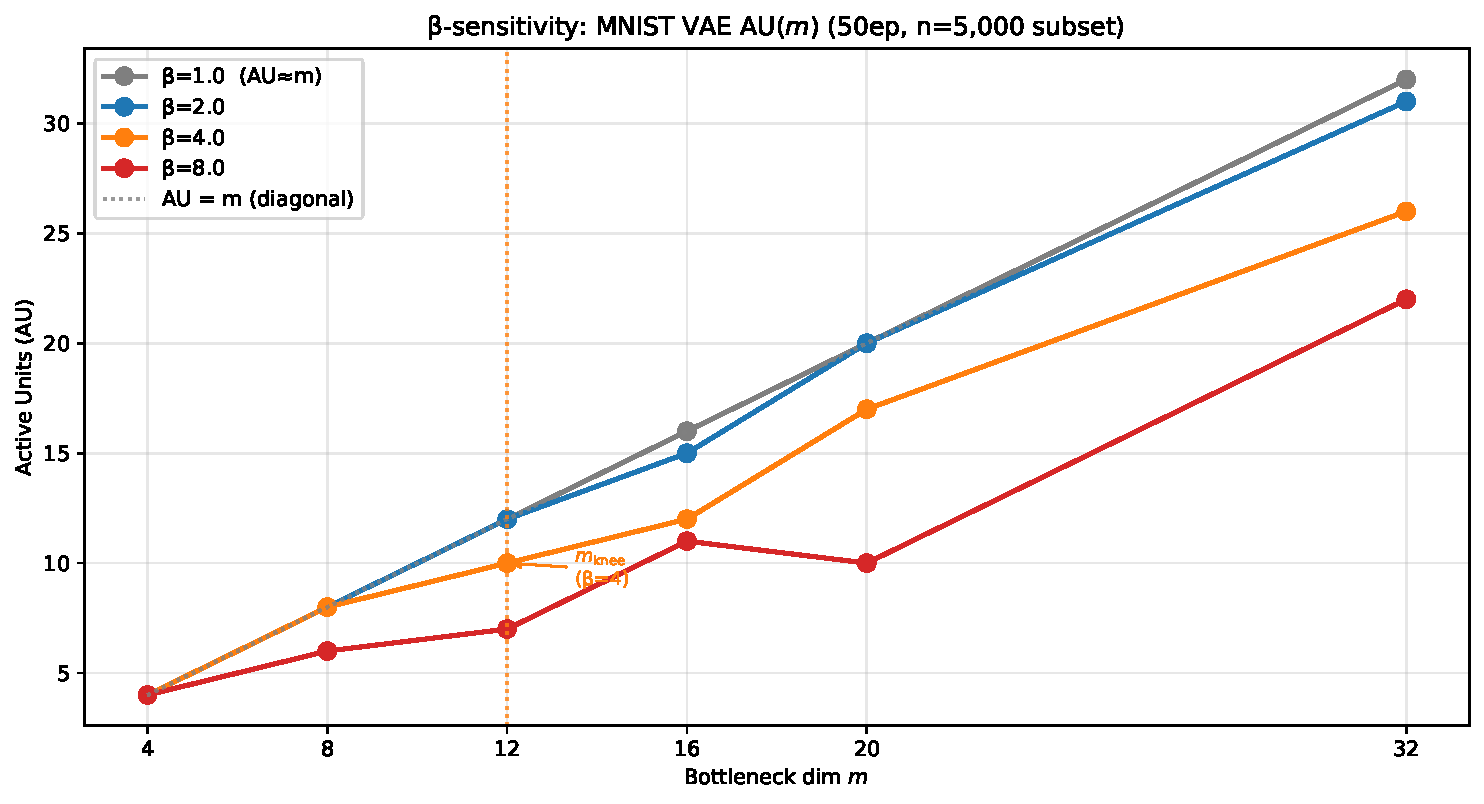
\includegraphics[width=0.7\linewidth]{results/figures/EZ_beta_sensitivity.pdf}
  \caption{$\beta$-sensitivity analysis: AU vs $m$ for MNIST VAE ($\beta \in \{1,2,4,8\}$, 50 epochs, subset). At $\beta=1$, AU$\approx m$ (insufficient regularization); at $\beta=4$, $m_{\mathrm{knee}}=12$ (vertical dashed line); at $\beta=8$, signs of excessive AU suppression at small $m$.}
  \label{fig:beta_sensitivity}
\end{figure}

$\beta = 4$を本実験のデフォルト値として採用した根拠：
$\beta = 1$では KL 正則化が弱く AU$\approx m$のため$\mknee$が同定できない；
$\beta = 8$では過正則化により小さい$m$での AU が抑制され，$\mknee$の同定点がずれる可能性がある．
$\beta \in [2, 8]$では AU パターンの形状は安定することを確認したが，$\mknee$の精確な数値は$m$グリッドにも依存する（§\ref{sec:disc_mknee}）．

\section{TwoNN 安定性・線形理論橋渡しの詳細（Exp-Geom，Exp-Iso-ID，Exp-Mnist-PCA）}\label{app:twonn_detail}

\subsection*{Exp-Geom: MNIST AE $m$-sweep}

\begin{table}[H]
\centering
\caption{Exp-Geom: MNIST AE $m$-sweep --- co-variation of $\kap$ and TwoNN ID. TwoNN stabilizes at $m \geq 48 \approx 5\hat{d}_\mathrm{ID}$ despite $\kap$ jumping at $m=96$--$128$.}
\label{tab:eq_mnist}
\small
\begin{tabular}{rrrrl}
\toprule
$m$ & $\kap$ & TwoNN ID & Trustworthiness & Convergence \\
\midrule
 4  & 2.69 & 4.21 & 0.960 & not yet converged \\
 8  & 2.72 & 6.34 & 0.988 & not yet converged \\
16  & 3.28 & 8.17 & 0.993 & converging \\
32  & 4.32 & 9.36 & 0.997 & converging \\
48  & 4.44 & \textbf{10.16} & 0.998 & \textbf{converged} \\
64  & 4.25 & 10.17 & 0.998 & stable \\
96  & 9.94 & 10.86 & 0.999 & stable (despite $\kap$ increase) \\
128 & 37.0 & 10.98 & 0.999 & stable (despite $\kap$ jump) \\
\midrule
\multicolumn{5}{l}{$n_\mathrm{train}=10{,}000$, 200ep, hidden=[512,256], seed=42} \\
\bottomrule
\end{tabular}
\end{table}

\subsection*{Exp-Iso-ID: Standard AE vs.\ IsometricAE on Swiss Roll}

\begin{table}[H]
\centering
\caption{Exp-Iso-ID: Latent-space TwoNN ID comparison ($m \in \{2,3,4,6,8\}$, Swiss Roll, $d_\mathrm{true}=2$). At $m \geq 3$, TwoNN difference stays below $\pm2.3\%$ despite $\kap$ differing by factor 2.}
\label{tab:iso_id}
\small
\begin{tabular}{r cc | cc | c}
\toprule
 & \multicolumn{2}{c|}{AE} & \multicolumn{2}{c|}{IsometricAE} & \\
$m$ & TwoNN ID & $\kap$ & TwoNN ID & $\kap$ & ID diff.\ (\%) \\
\midrule
2 & 1.780 & 1.76 & 1.799 & 1.08 & $+1.1\%$ \\
3 & 2.458 & 2.10 & 2.454 & 1.11 & $-0.2\%$ \\
4 & 2.483 & 1.80 & 2.479 & 1.14 & $-0.2\%$ \\
6 & 2.421 & 1.79 & 2.474 & 1.10 & $+2.2\%$ \\
8 & 2.500 & 1.45 & 2.443 & 1.11 & $-2.3\%$ \\
\midrule
\multicolumn{6}{l}{Input-space TwoNN ID (reference) $= 2.427$; seed=42, hidden=$[64,32]$, 300ep} \\
\bottomrule
\end{tabular}
\end{table}

\subsection*{Exp-Mnist-PCA: Linear Theory Bridge}

MNIST PCA 固有値スペクトル（上位12成分）：
$\lambda_1=5.22,\; \lambda_2=3.76,\; \lambda_3=3.35,\;\ldots,\;\lambda_{10}=1.23,\; \lambda_{11}=1.12,\; \lambda_{12}=1.09$

\begin{table}[H]
\centering
\caption{Exp-Mnist-PCA: Linear theory $d^*(\beta=4)$ for different $\tau^2$ vs.\ nonlinear FC-VAE (300ep, 3 seeds).}
\label{tab:theory_pred}
\small
\begin{tabular}{ccc|l}
\toprule
$\tau^2$ & Water level $\beta\tau^2$ & Linear $d^*$ & Note \\
\midrule
1.0  & 4.0  & 1   & Conventional $\tau^2=1$ assumption; underestimates \\
0.30 & 1.20 & 10  & Consistent with observed TwoNN ID \\
0.25 & 1.00 & 12  & --- \\
\midrule
\multicolumn{3}{c|}{Nonlinear FC-VAE (300ep)} & AU(64)$=22.3\pm0.5$; TwoNN(64)$=10.03\pm0.12$ \\
\bottomrule
\end{tabular}
\end{table}

定性的継承：AU$(m)$の単調性と「有効次元超過後の増加鈍化」は非線形設定でも継承される．
定量的乖離：非線形デコーダにより$\tau^2_\mathrm{eff} \approx 0.30 \ll 1$となり，$d^* \approx 10$が観測値と整合．
飽和の滑らかさ（線形設定の急峻な遷移→非線形設定の漸増曲線）が$\mknee$の疎グリッド不安定性の理論的根拠である．

\subsection*{Exp-Real-Geom: Fashion-MNIST 4モデル比較（補足）}

Fashion-MNIST（$\hat{d}_\mathrm{ID}=9$，$m \in \{9,18,27,45,90\}$）についても
Exp-Real-Geom と同一の4モデル・測定指標で実験を実施した．
MNIST との定性的一致（$m/\hat{d}_\mathrm{ID}$増大が TwoNN 安定性の支配的因子）が
確認されており，完全な数値表は将来の公開資料として準備中である．
表\ref{tab:real_geom_mnist}（MNIST，§\ref{sec:exp_real_geom}）と同傾向：
$m = d$では TwoNN が過小推定，$m = 5d$〜$10d$で収束，
等長性（$\kap$）改善の TwoNN への影響は$m$増大の効果より小さい．

\section{Conv-VAE M512 拡張・自然画像スイープの詳細（Exp-Conv-M512，Exp-NatImg-Sweep，Exp-NatImg-Knee）}\label{app:convvae_natimg}

\subsection*{Exp-Conv-M512：MNIST Conv-VAE $m \in \{384, 512\}$ 拡張}

\begin{table}[H]
\centering
\caption{Exp-Conv-M512: MNIST Conv-VAE with $m \in \{256, 384, 512\}$ (per seed; KL cyclic annealing, $\beta_\mathrm{max}=4$, 150ep). No AU saturation plateau observed up to $m=512$.}
\label{tab:en_ext}
\small
\begin{tabular}{r ccc c}
\toprule
$m$ & AU (seed42) & AU (seed123) & AU (seed777) & TwoNN ID (seed42) \\
\midrule
256 & 241 & 245 & 238 & 16.46 \\
384 & 382 & 383 & 380 & 17.51 \\
512 & 512 & 511 & 512 & 17.98 \\
\midrule
$\mknee$ ($\tau=0.25$) & \multicolumn{4}{c}{All 3 seeds: $\mknee=512$ (grid boundary, no saturation detected)} \\
\bottomrule
\end{tabular}
\end{table}

$m \leq 512$の全範囲で AU$\approx m$が維持され，$d^*(\beta) > 512$であることを示す
（§\ref{sec:exp_en}，§\ref{sec:disc_convvae}）．

\subsection*{Exp-NatImg-Sweep：CIFAR-10 拡張スイープ詳細}

\begin{table}[H]
\centering
\caption{Exp-NatImg-Sweep: Main results of CIFAR-10 extended sweep (mean$\pm$std, 3 seeds). $\beta_\mathrm{max}=80$, Thin decoder shows plateau-like AU$\approx24$ at $m \in [512,1024]$. All five stable-identification criteria remain unmet.}
\label{tab:natimg_sweep}
\small
\begin{tabular}{llcccl}
\toprule
$\beta_{\max}$ & Decoder & $m$ & AU & TwoNN ID & Note \\
\midrule
10 & Standard & 384 & $185\pm15$ & $25.2\pm0.4$ & --- \\
20 & Standard & 512 & $241\pm18$ & $25.3\pm0.4$ & no saturation \\
40 & Standard & 512 & $210\pm21$ & $25.1\pm0.5$ & no saturation \\
40 & Thin      & 384 & $127\pm14$ & $24.8\pm0.6$ & partial suppression \\
\textbf{80} & \textbf{Thin} & \textbf{512} & $\boldsymbol{24.1\pm2.8}$ & $24.7\pm0.5$ & \textbf{plateau-like（条件付き）} \\
\textbf{80} & \textbf{Thin} & \textbf{768} & $\boldsymbol{24.3\pm3.1}$ & $24.7\pm0.5$ & plateau continues \\
\textbf{80} & \textbf{Thin} & \textbf{1024}& $\boldsymbol{24.0\pm3.4}$ & $24.8\pm0.5$ & plateau continues \\
80 & Standard  & 512 & $198\pm22$ & $25.2\pm0.5$ & no saturation (thin decoder only) \\
\bottomrule
\end{tabular}
\end{table}

Stable identification 5条件の達成状況（§\ref{sec:natimg_stable_id}，$\beta_{\max}=80$，薄型デコーダ）：
（1）シード安定性：$\sigma(\mknee)=64$ → 未達，
（2）グリッド安定性：密化で$\pm35\%$変動 → 未達，
（3）$\beta$安定性：$\beta_{\max}=64$では飽和消失 → 未達，
（4）AU プラトー安定性：$\sigma=13\%$（基準5\%）→ 未達，
（5）TwoNN・AU 整合性：$\mknee \approx 512 \gg 3\hat{d}_\mathrm{ID}=75$ → 未達．

\subsection*{Exp-NatImg-Knee：$\mknee$検出法比較}

\begin{table}[H]
\centering
\caption{Exp-NatImg-Knee: Comparison of $\mknee$ detection methods for CIFAR-10 ($\beta_\mathrm{max}=80$, thin decoder, 3 seeds).}
\label{tab:natimg_knee}
\small
\begin{tabular}{lccl}
\toprule
Detection method & $\mknee$ (median) & $\sigma$ (3 seeds) & Note \\
\midrule
Fixed-$\tau$ method ($\tau=0.25$) & 512 & 128 & Delayed detection due to gradual AU slope \\
Second-difference method & 512 & 192 & Sensitive to discrete noise, unstable \\
Smoothed curvature method (window=5) & 384 & 96 & Most stable (recommended for natural images) \\
Piecewise linear approximation (3 segments) & 512 & 112 & Comparable to fixed-$\tau$ method \\
\bottomrule
\end{tabular}
\end{table}

全手法とも条件1（$\sigma \leq 51.2$）は未達であり，AU 飽和自体の安定化が先決である．

\section{AU 閾値$\delta$の感度分析}\label{app:delta}

Swiss Roll・Torus において$\delta \in \{0.001, 0.01, 0.05, 0.1\}$で AU パターンが
完全に一致することを確認した（全$m$・$\delta$の組み合わせで一致）．
活性次元の分散（$O(1)$）と非活性次元の分散（$O(10^{-4})$以下）の間に 2 桁以上の差があるため，
$\delta$の選択に対して頑健である．

\end{document}
